\documentclass[twoside]{book}

% Packages required by doxygen
\usepackage{fixltx2e}
\usepackage{calc}
\usepackage{doxygen}
\usepackage[export]{adjustbox} % also loads graphicx
\usepackage{graphicx}
\usepackage[utf8]{inputenc}
\usepackage{makeidx}
\usepackage{multicol}
\usepackage{multirow}
\PassOptionsToPackage{warn}{textcomp}
\usepackage{textcomp}
\usepackage[nointegrals]{wasysym}
\usepackage[table]{xcolor}

% Font selection
\usepackage[T1]{fontenc}
\usepackage[scaled=.90]{helvet}
\usepackage{courier}
\usepackage{amssymb}
\usepackage{sectsty}
\renewcommand{\familydefault}{\sfdefault}
\allsectionsfont{%
  \fontseries{bc}\selectfont%
  \color{darkgray}%
}
\renewcommand{\DoxyLabelFont}{%
  \fontseries{bc}\selectfont%
  \color{darkgray}%
}
\newcommand{\+}{\discretionary{\mbox{\scriptsize$\hookleftarrow$}}{}{}}

% Page & text layout
\usepackage{geometry}
\geometry{%
  a4paper,%
  top=2.5cm,%
  bottom=2.5cm,%
  left=2.5cm,%
  right=2.5cm%
}
\tolerance=750
\hfuzz=15pt
\hbadness=750
\setlength{\emergencystretch}{15pt}
\setlength{\parindent}{0cm}
\setlength{\parskip}{3ex plus 2ex minus 2ex}
\makeatletter
\renewcommand{\paragraph}{%
  \@startsection{paragraph}{4}{0ex}{-1.0ex}{1.0ex}{%
    \normalfont\normalsize\bfseries\SS@parafont%
  }%
}
\renewcommand{\subparagraph}{%
  \@startsection{subparagraph}{5}{0ex}{-1.0ex}{1.0ex}{%
    \normalfont\normalsize\bfseries\SS@subparafont%
  }%
}
\makeatother

% Headers & footers
\usepackage{fancyhdr}
\pagestyle{fancyplain}
\fancyhead[LE]{\fancyplain{}{\bfseries\thepage}}
\fancyhead[CE]{\fancyplain{}{}}
\fancyhead[RE]{\fancyplain{}{\bfseries\leftmark}}
\fancyhead[LO]{\fancyplain{}{\bfseries\rightmark}}
\fancyhead[CO]{\fancyplain{}{}}
\fancyhead[RO]{\fancyplain{}{\bfseries\thepage}}
\fancyfoot[LE]{\fancyplain{}{}}
\fancyfoot[CE]{\fancyplain{}{}}
\fancyfoot[RE]{\fancyplain{}{\bfseries\scriptsize Generated by Doxygen }}
\fancyfoot[LO]{\fancyplain{}{\bfseries\scriptsize Generated by Doxygen }}
\fancyfoot[CO]{\fancyplain{}{}}
\fancyfoot[RO]{\fancyplain{}{}}
\renewcommand{\footrulewidth}{0.4pt}
\renewcommand{\chaptermark}[1]{%
  \markboth{#1}{}%
}
\renewcommand{\sectionmark}[1]{%
  \markright{\thesection\ #1}%
}

% Indices & bibliography
\usepackage{natbib}
\usepackage[titles]{tocloft}
\setcounter{tocdepth}{3}
\setcounter{secnumdepth}{5}
\makeindex

% Hyperlinks (required, but should be loaded last)
\usepackage{ifpdf}
\ifpdf
  \usepackage[pdftex,pagebackref=true]{hyperref}
\else
  \usepackage[ps2pdf,pagebackref=true]{hyperref}
\fi
\hypersetup{%
  colorlinks=true,%
  linkcolor=blue,%
  citecolor=blue,%
  unicode%
}

% Custom commands
\newcommand{\clearemptydoublepage}{%
  \newpage{\pagestyle{empty}\cleardoublepage}%
}

\usepackage{caption}
\captionsetup{labelsep=space,justification=centering,font={bf},singlelinecheck=off,skip=4pt,position=top}

%===== C O N T E N T S =====

\begin{document}

% Titlepage & ToC
\hypersetup{pageanchor=false,
             bookmarksnumbered=true,
             pdfencoding=unicode
            }
\pagenumbering{alph}
\begin{titlepage}
\vspace*{7cm}
\begin{center}%
{\Large Raytracer \\[1ex]\large 0.\+1 }\\
\vspace*{1cm}
{\large Generated by Doxygen 1.8.13}\\
\end{center}
\end{titlepage}
\clearemptydoublepage
\pagenumbering{roman}
\tableofcontents
\clearemptydoublepage
\pagenumbering{arabic}
\hypersetup{pageanchor=true}

%--- Begin generated contents ---
\chapter{Namespace Index}
\section{Namespace List}
Here is a list of all documented namespaces with brief descriptions\+:\begin{DoxyCompactList}
\item\contentsline{section}{\hyperlink{namespaceraytracer}{raytracer} \\*Namespace of the whole library }{\pageref{namespaceraytracer}}{}
\item\contentsline{section}{\hyperlink{namespaceraytracer_1_1geometry}{raytracer\+::geometry} \\*Namespace encapsulating all the abstractions related to geometry }{\pageref{namespaceraytracer_1_1geometry}}{}
\item\contentsline{section}{\hyperlink{namespaceraytracer_1_1geometry_1_1constants}{raytracer\+::geometry\+::constants} \\*Namespace encapsulating geometry constants }{\pageref{namespaceraytracer_1_1geometry_1_1constants}}{}
\item\contentsline{section}{\hyperlink{namespaceraytracer_1_1physics_1_1constants}{raytracer\+::physics\+::constants} \\*Basic physics constants in cgs units }{\pageref{namespaceraytracer_1_1physics_1_1constants}}{}
\end{DoxyCompactList}

\chapter{Hierarchical Index}
\section{Class Hierarchy}
This inheritance list is sorted roughly, but not completely, alphabetically\+:\begin{DoxyCompactList}
\item \contentsline{section}{raytracer\+:\+:physics\+:\+:Collisional\+Frequency\+Calculator}{\pageref{classraytracer_1_1physics_1_1CollisionalFrequencyCalculator}}{}
\begin{DoxyCompactList}
\item \contentsline{section}{raytracer\+:\+:physics\+:\+:Spitzer\+Frequency\+Calculator}{\pageref{classraytracer_1_1physics_1_1SpitzerFrequencyCalculator}}{}
\end{DoxyCompactList}
\item \contentsline{section}{raytracer\+:\+:physics\+:\+:Continue\+Straight}{\pageref{structraytracer_1_1physics_1_1ContinueStraight}}{}
\item \contentsline{section}{raytracer\+:\+:physics\+:\+:Density}{\pageref{structraytracer_1_1physics_1_1Density}}{}
\item \contentsline{section}{raytracer\+:\+:geometry\+:\+:Discrete\+Line}{\pageref{structraytracer_1_1geometry_1_1DiscreteLine}}{}
\item \contentsline{section}{raytracer\+:\+:physics\+:\+:Dont\+Stop}{\pageref{structraytracer_1_1physics_1_1DontStop}}{}
\item \contentsline{section}{raytracer\+:\+:geometry\+:\+:Element}{\pageref{classraytracer_1_1geometry_1_1Element}}{}
\item \contentsline{section}{raytracer\+:\+:physics\+:\+:Energy}{\pageref{structraytracer_1_1physics_1_1Energy}}{}
\item \contentsline{section}{raytracer\+:\+:geometry\+:\+:Face}{\pageref{classraytracer_1_1geometry_1_1Face}}{}
\item \contentsline{section}{raytracer\+:\+:physics\+:\+:Frequency}{\pageref{structraytracer_1_1physics_1_1Frequency}}{}
\item \contentsline{section}{raytracer\+:\+:physics\+:\+:Gaussian}{\pageref{classraytracer_1_1physics_1_1Gaussian}}{}
\item \contentsline{section}{raytracer\+:\+:physics\+:\+:Gradient\+Calculator}{\pageref{classraytracer_1_1physics_1_1GradientCalculator}}{}
\begin{DoxyCompactList}
\item \contentsline{section}{raytracer\+:\+:physics\+:\+:Constant\+Gradient\+Calculator}{\pageref{classraytracer_1_1physics_1_1ConstantGradientCalculator}}{}
\item \contentsline{section}{raytracer\+:\+:physics\+:\+:H1\+Gradient\+Calculator}{\pageref{classraytracer_1_1physics_1_1H1GradientCalculator}}{}
\end{DoxyCompactList}
\item \contentsline{section}{raytracer\+:\+:geometry\+:\+:Half\+Line}{\pageref{structraytracer_1_1geometry_1_1HalfLine}}{}
\item \contentsline{section}{raytracer\+:\+:geometry\+:\+:Intersection}{\pageref{structraytracer_1_1geometry_1_1Intersection}}{}
\item \contentsline{section}{raytracer\+:\+:physics\+:\+:Laser}{\pageref{classraytracer_1_1physics_1_1Laser}}{}
\item \contentsline{section}{raytracer\+:\+:physics\+:\+:Laser\+Ray}{\pageref{structraytracer_1_1physics_1_1LaserRay}}{}
\item \contentsline{section}{raytracer\+:\+:physics\+:\+:Length}{\pageref{structraytracer_1_1physics_1_1Length}}{}
\item \contentsline{section}{raytracer\+:\+:geometry\+:\+:Mesh}{\pageref{classraytracer_1_1geometry_1_1Mesh}}{}
\item \contentsline{section}{raytracer\+:\+:geometry\+:\+:Mesh\+Function}{\pageref{classraytracer_1_1geometry_1_1MeshFunction}}{}
\begin{DoxyCompactList}
\item \contentsline{section}{raytracer\+:\+:geometry\+:\+:Mfem\+Mesh\+Function}{\pageref{classraytracer_1_1geometry_1_1MfemMeshFunction}}{}
\end{DoxyCompactList}
\item \contentsline{section}{raytracer\+:\+:geometry\+:\+:Point}{\pageref{classraytracer_1_1geometry_1_1Point}}{}
\item \contentsline{section}{raytracer\+:\+:geometry\+:\+:Ray}{\pageref{classraytracer_1_1geometry_1_1Ray}}{}
\item \contentsline{section}{raytracer\+:\+:physics\+:\+:Snells\+Law}{\pageref{structraytracer_1_1physics_1_1SnellsLaw}}{}
\item \contentsline{section}{raytracer\+:\+:physics\+:\+:Stop\+At\+Critical}{\pageref{structraytracer_1_1physics_1_1StopAtCritical}}{}
\item \contentsline{section}{raytracer\+:\+:physics\+:\+:Temperature}{\pageref{structraytracer_1_1physics_1_1Temperature}}{}
\item \contentsline{section}{raytracer\+:\+:geometry\+:\+:Vector}{\pageref{classraytracer_1_1geometry_1_1Vector}}{}
\end{DoxyCompactList}

\chapter{Class Index}
\section{Class List}
Here are the classes, structs, unions and interfaces with brief descriptions\+:\begin{DoxyCompactList}
\item\contentsline{section}{\hyperlink{classraytracer_1_1AbsorptionController}{raytracer\+::\+Absorption\+Controller} \\*Class aggregating all instances of \hyperlink{classraytracer_1_1AbsorptionModel}{Absorption\+Model} used to update absorbed\+Energy mesh\+Function }{\pageref{classraytracer_1_1AbsorptionController}}{}
\item\contentsline{section}{\hyperlink{classraytracer_1_1AbsorptionModel}{raytracer\+::\+Absorption\+Model} \\*Abstract interface, to obey this get\+Energy\+Change must be implemented }{\pageref{classraytracer_1_1AbsorptionModel}}{}
\item\contentsline{section}{\hyperlink{structraytracer_1_1Bremsstrahlung}{raytracer\+::\+Bremsstrahlung} \\*Absorption model of energy exchange due to bremsstrahlung }{\pageref{structraytracer_1_1Bremsstrahlung}}{}
\item\contentsline{section}{\hyperlink{classraytracer_1_1CollisionalFrequency}{raytracer\+::\+Collisional\+Frequency} \\*Abstract interface }{\pageref{classraytracer_1_1CollisionalFrequency}}{}
\item\contentsline{section}{\hyperlink{classraytracer_1_1ConstantGradient}{raytracer\+::\+Constant\+Gradient} \\*Gradient\+Calculator that returns a constant \hyperlink{classraytracer_1_1Vector}{Vector} no matter what }{\pageref{classraytracer_1_1ConstantGradient}}{}
\item\contentsline{section}{\hyperlink{structraytracer_1_1ContinueStraight}{raytracer\+::\+Continue\+Straight} \\*Functor that returns always the previous\+Direction }{\pageref{structraytracer_1_1ContinueStraight}}{}
\item\contentsline{section}{\hyperlink{structraytracer_1_1Density}{raytracer\+::\+Density} \\*Strong type representing length in cm$^\wedge$-\/3 }{\pageref{structraytracer_1_1Density}}{}
\item\contentsline{section}{\hyperlink{structraytracer_1_1DiscreteLine}{raytracer\+::\+Discrete\+Line} \\*Structure representing a discretization of a distance }{\pageref{structraytracer_1_1DiscreteLine}}{}
\item\contentsline{section}{\hyperlink{structraytracer_1_1DontStop}{raytracer\+::\+Dont\+Stop} \\*Functor for ray propagation that returns false in any case }{\pageref{structraytracer_1_1DontStop}}{}
\item\contentsline{section}{\hyperlink{classraytracer_1_1Element}{raytracer\+::\+Element} \\*Class representing a single polygonal element in mesh }{\pageref{classraytracer_1_1Element}}{}
\item\contentsline{section}{\hyperlink{structraytracer_1_1Energy}{raytracer\+::\+Energy} \\*Strong type representing energy in joules }{\pageref{structraytracer_1_1Energy}}{}
\item\contentsline{section}{\hyperlink{classraytracer_1_1Face}{raytracer\+::\+Face} \\*Class representing a polygonal face in mesh (edge in 2D, surface polygon face in 3D) }{\pageref{classraytracer_1_1Face}}{}
\item\contentsline{section}{\hyperlink{structraytracer_1_1Frequency}{raytracer\+::\+Frequency} \\*Strong type representing frequency in s$^\wedge$-\/1 }{\pageref{structraytracer_1_1Frequency}}{}
\item\contentsline{section}{\hyperlink{classraytracer_1_1Gaussian}{raytracer\+::\+Gaussian} \\*Class representing a 1D gaussian with given parametrs }{\pageref{classraytracer_1_1Gaussian}}{}
\item\contentsline{section}{\hyperlink{classraytracer_1_1Gradient}{raytracer\+::\+Gradient} \\*Abstract interface to provide a Gradient\+Calculator }{\pageref{classraytracer_1_1Gradient}}{}
\item\contentsline{section}{\hyperlink{classraytracer_1_1H1Gradient}{raytracer\+::\+H1\+Gradient} \\*Gradient\+Calculator that stores a density grid function defined in H1 space obtained from function given if L2 }{\pageref{classraytracer_1_1H1Gradient}}{}
\item\contentsline{section}{\hyperlink{structraytracer_1_1HalfLine}{raytracer\+::\+Half\+Line} \\*Structure representing a half line }{\pageref{structraytracer_1_1HalfLine}}{}
\item\contentsline{section}{\hyperlink{structraytracer_1_1Intersection}{raytracer\+::\+Intersection} \\*Structure representing a single intersection of \hyperlink{classraytracer_1_1Ray}{Ray} with a \hyperlink{classraytracer_1_1Mesh}{Mesh} }{\pageref{structraytracer_1_1Intersection}}{}
\item\contentsline{section}{\hyperlink{classraytracer_1_1Laser}{raytracer\+::\+Laser} \\*Class representing a real physical laser }{\pageref{classraytracer_1_1Laser}}{}
\item\contentsline{section}{\hyperlink{classraytracer_1_1LaserRay}{raytracer\+::\+Laser\+Ray} \\*Class representing a single \hyperlink{classraytracer_1_1LaserRay}{Laser\+Ray} }{\pageref{classraytracer_1_1LaserRay}}{}
\item\contentsline{section}{\hyperlink{structraytracer_1_1Length}{raytracer\+::\+Length} \\*Strong type representing length in cm }{\pageref{structraytracer_1_1Length}}{}
\item\contentsline{section}{\hyperlink{classraytracer_1_1Mesh}{raytracer\+::\+Mesh} \\*Class representing a mesh (2D for now) }{\pageref{classraytracer_1_1Mesh}}{}
\item\contentsline{section}{\hyperlink{classraytracer_1_1MeshFunction}{raytracer\+::\+Mesh\+Function} \\*Abstract interface }{\pageref{classraytracer_1_1MeshFunction}}{}
\item\contentsline{section}{\hyperlink{classraytracer_1_1MfemMeshFunction}{raytracer\+::\+Mfem\+Mesh\+Function} \\*Discrete function what has constant values at \hyperlink{classraytracer_1_1Mesh}{Mesh} elements }{\pageref{classraytracer_1_1MfemMeshFunction}}{}
\item\contentsline{section}{\hyperlink{classraytracer_1_1Point}{raytracer\+::\+Point} \\*Class representing a point A point is given by two coordinates x and y }{\pageref{classraytracer_1_1Point}}{}
\item\contentsline{section}{\hyperlink{structraytracer_1_1PointOnFace}{raytracer\+::\+Point\+On\+Face} \\*Structure representing a point on a face }{\pageref{structraytracer_1_1PointOnFace}}{}
\item\contentsline{section}{\hyperlink{classraytracer_1_1Ray}{raytracer\+::\+Ray} \\*Class representing a ray propagating through \hyperlink{classraytracer_1_1Mesh}{Mesh} }{\pageref{classraytracer_1_1Ray}}{}
\item\contentsline{section}{\hyperlink{structraytracer_1_1SnellsLaw}{raytracer\+::\+Snells\+Law} \\*Functor that finds new direction base on the Snells\textquotesingle{}s law }{\pageref{structraytracer_1_1SnellsLaw}}{}
\item\contentsline{section}{\hyperlink{classraytracer_1_1SpitzerFrequency}{raytracer\+::\+Spitzer\+Frequency} \\*Class representing a Spitzer-\/\+Harm frequency calculator }{\pageref{classraytracer_1_1SpitzerFrequency}}{}
\item\contentsline{section}{\hyperlink{classraytracer_1_1StepGradient}{raytracer\+::\+Step\+Gradient} \\*Gradient\+Calculator that returns the normal to the face as \hyperlink{classraytracer_1_1Gradient}{Gradient} }{\pageref{classraytracer_1_1StepGradient}}{}
\item\contentsline{section}{\hyperlink{structraytracer_1_1StopAtCritical}{raytracer\+::\+Stop\+At\+Critical} \\*Functor for ray propagation termination based on critical density expected to used with lase\+Ray intersection finding procedure }{\pageref{structraytracer_1_1StopAtCritical}}{}
\item\contentsline{section}{\hyperlink{structraytracer_1_1Temperature}{raytracer\+::\+Temperature} \\*Strong type representing temperature in eV }{\pageref{structraytracer_1_1Temperature}}{}
\item\contentsline{section}{\hyperlink{classraytracer_1_1Vector}{raytracer\+::\+Vector} \\*Class representing a physical vector }{\pageref{classraytracer_1_1Vector}}{}
\end{DoxyCompactList}

\chapter{Namespace Documentation}
\hypertarget{namespaceraytracer}{}\section{raytracer Namespace Reference}
\label{namespaceraytracer}\index{raytracer@{raytracer}}


Namespace of the whole library.  


\subsection*{Namespaces}
\begin{DoxyCompactItemize}
\item 
 \hyperlink{namespaceraytracer_1_1geometry}{geometry}
\begin{DoxyCompactList}\small\item\em Namespace encapsulating all the abstractions related to geometry. \end{DoxyCompactList}\end{DoxyCompactItemize}


\subsection{Detailed Description}
Namespace of the whole library. 
\hypertarget{namespaceraytracer_1_1geometry}{}\section{raytracer\+:\+:geometry Namespace Reference}
\label{namespaceraytracer_1_1geometry}\index{raytracer\+::geometry@{raytracer\+::geometry}}


Namespace encapsulating all the abstractions related to geometry.  


\subsection*{Namespaces}
\begin{DoxyCompactItemize}
\item 
 \hyperlink{namespaceraytracer_1_1geometry_1_1constants}{constants}
\begin{DoxyCompactList}\small\item\em Namespace encapsulating geometry constants. \end{DoxyCompactList}\end{DoxyCompactItemize}
\subsection*{Classes}
\begin{DoxyCompactItemize}
\item 
struct \hyperlink{structraytracer_1_1geometry_1_1DiscreteLine}{Discrete\+Line}
\begin{DoxyCompactList}\small\item\em Structure representing a discretisation of a distance. \end{DoxyCompactList}\item 
class \hyperlink{classraytracer_1_1geometry_1_1Element}{Element}
\begin{DoxyCompactList}\small\item\em Class representing a single volume element in mesh. \end{DoxyCompactList}\item 
class \hyperlink{classraytracer_1_1geometry_1_1Face}{Face}
\begin{DoxyCompactList}\small\item\em Class representing a face in mesh (edge in 2D, surface face in 3D). \end{DoxyCompactList}\item 
struct \hyperlink{structraytracer_1_1geometry_1_1HalfLine}{Half\+Line}
\begin{DoxyCompactList}\small\item\em Structure representing a half line. \end{DoxyCompactList}\item 
struct \hyperlink{structraytracer_1_1geometry_1_1Intersection}{Intersection}
\begin{DoxyCompactList}\small\item\em Structure representing a single intersection of \hyperlink{structraytracer_1_1geometry_1_1HalfLine}{Half\+Line} with a mesh. \end{DoxyCompactList}\item 
class \hyperlink{classraytracer_1_1geometry_1_1Mesh}{Mesh}
\begin{DoxyCompactList}\small\item\em Class representing a mesh. \end{DoxyCompactList}\item 
class \hyperlink{classraytracer_1_1geometry_1_1MeshFunction}{Mesh\+Function}
\begin{DoxyCompactList}\small\item\em Abstract interface. \end{DoxyCompactList}\item 
class \hyperlink{classraytracer_1_1geometry_1_1MfemMeshFunction}{Mfem\+Mesh\+Function}
\begin{DoxyCompactList}\small\item\em Wrapper class around mfem\+::\+Grid\+Function. \end{DoxyCompactList}\item 
class \hyperlink{classraytracer_1_1geometry_1_1Point}{Point}
\begin{DoxyCompactList}\small\item\em Class representing a point A point is given by two coordinates x and y. \end{DoxyCompactList}\item 
class \hyperlink{classraytracer_1_1geometry_1_1Ray}{Ray}
\begin{DoxyCompactList}\small\item\em Class representing a ray propagating through mesh. \end{DoxyCompactList}\item 
class \hyperlink{classraytracer_1_1geometry_1_1Vector}{Vector}
\begin{DoxyCompactList}\small\item\em Class representing a physical vector. \end{DoxyCompactList}\end{DoxyCompactItemize}
\subsection*{Functions}
\begin{DoxyCompactItemize}
\item 
std\+::unique\+\_\+ptr$<$ \hyperlink{structraytracer_1_1geometry_1_1Intersection}{Intersection} $>$ \hyperlink{namespaceraytracer_1_1geometry_aef0f9f1bd82ffb69b8d6343a57106234}{find\+Intersection} (const \hyperlink{structraytracer_1_1geometry_1_1HalfLine}{Half\+Line} \&half\+Line, const \hyperlink{classraytracer_1_1geometry_1_1Face}{Face} $\ast$face)
\begin{DoxyCompactList}\small\item\em Find an intersection of \hyperlink{structraytracer_1_1geometry_1_1HalfLine}{Half\+Line} with a face. \end{DoxyCompactList}\item 
std\+::unique\+\_\+ptr$<$ \hyperlink{structraytracer_1_1geometry_1_1Intersection}{Intersection} $>$ \hyperlink{namespaceraytracer_1_1geometry_ae05eacb910ded12afa671c5563e91b11}{find\+Closest\+Intersection} (const \hyperlink{structraytracer_1_1geometry_1_1HalfLine}{Half\+Line} \&half\+Line, const std\+::vector$<$ \hyperlink{classraytracer_1_1geometry_1_1Face}{Face} $\ast$$>$ \&faces, const \hyperlink{classraytracer_1_1geometry_1_1Face}{Face} $\ast$omit\+Face=nullptr)
\begin{DoxyCompactList}\small\item\em For a given set of faces find all its intersections with a \hyperlink{structraytracer_1_1geometry_1_1HalfLine}{Half\+Line} and return the one that is closest to the origin of the \hyperlink{structraytracer_1_1geometry_1_1HalfLine}{Half\+Line}. \end{DoxyCompactList}\item 
std\+::unique\+\_\+ptr$<$ mfem\+::\+Mesh $>$ \hyperlink{namespaceraytracer_1_1geometry_a8d4b7f6d4fec35e4deeb09ec86b3d140}{construct\+Rectangle\+Mesh} (\hyperlink{structraytracer_1_1geometry_1_1DiscreteLine}{Discrete\+Line} sideA, \hyperlink{structraytracer_1_1geometry_1_1DiscreteLine}{Discrete\+Line} sideB)
\begin{DoxyCompactList}\small\item\em Construct a mfem\+::\+Mesh given two discrete lines (the sides of the rectangle). \end{DoxyCompactList}\item 
const \hyperlink{classraytracer_1_1geometry_1_1Vector}{Vector} \hyperlink{namespaceraytracer_1_1geometry_a019177298d61bc227f55b0d51a83f60e}{operator-\/} (\hyperlink{classraytracer_1_1geometry_1_1Point}{Point} A, \hyperlink{classraytracer_1_1geometry_1_1Point}{Point} B)
\begin{DoxyCompactList}\small\item\em Two Points can be subtracted to get a \hyperlink{classraytracer_1_1geometry_1_1Vector}{Vector}. \end{DoxyCompactList}\item 
const \hyperlink{classraytracer_1_1geometry_1_1Point}{Point} \hyperlink{namespaceraytracer_1_1geometry_aa576460b4f567015830e98247c12f3ce}{operator+} (\hyperlink{classraytracer_1_1geometry_1_1Point}{Point} A, \hyperlink{classraytracer_1_1geometry_1_1Vector}{Vector} b)
\begin{DoxyCompactList}\small\item\em \hyperlink{classraytracer_1_1geometry_1_1Vector}{Vector} and point can be added get another point. \end{DoxyCompactList}\item 
const \hyperlink{classraytracer_1_1geometry_1_1Point}{Point} \hyperlink{namespaceraytracer_1_1geometry_aaf48be2ee020c2f48557c6361dfd64d1}{operator+} (\hyperlink{classraytracer_1_1geometry_1_1Vector}{Vector} b, \hyperlink{classraytracer_1_1geometry_1_1Point}{Point} A)
\begin{DoxyCompactList}\small\item\em Convenience wrapper around A + b. \end{DoxyCompactList}\item 
const \hyperlink{classraytracer_1_1geometry_1_1Vector}{Vector} \hyperlink{namespaceraytracer_1_1geometry_ada5477612107be5f59456de8524caa97}{operator$\ast$} (double k, \hyperlink{classraytracer_1_1geometry_1_1Vector}{Vector} a)
\begin{DoxyCompactList}\small\item\em \hyperlink{classraytracer_1_1geometry_1_1Vector}{Vector} can be multiplied by number k$\ast$a. \end{DoxyCompactList}\item 
const \hyperlink{classraytracer_1_1geometry_1_1Vector}{Vector} \hyperlink{namespaceraytracer_1_1geometry_a3030b86be5d83356f089b60e3465ee12}{operator$\ast$} (\hyperlink{classraytracer_1_1geometry_1_1Vector}{Vector} a, double k)
\begin{DoxyCompactList}\small\item\em Convenience wrapper around k$\ast$a. \end{DoxyCompactList}\item 
double \hyperlink{namespaceraytracer_1_1geometry_a11b9e4ba4dc8bcc091387d4a7934ab7e}{operator$\ast$} (\hyperlink{classraytracer_1_1geometry_1_1Vector}{Vector} a, \hyperlink{classraytracer_1_1geometry_1_1Vector}{Vector} b)
\begin{DoxyCompactList}\small\item\em his is the dot product of two vectors a, b \end{DoxyCompactList}\item 
const \hyperlink{classraytracer_1_1geometry_1_1Vector}{Vector} \hyperlink{namespaceraytracer_1_1geometry_a43e318baa7b3ea626fcf42c80f2e86c4}{operator+} (\hyperlink{classraytracer_1_1geometry_1_1Vector}{Vector} a, \hyperlink{classraytracer_1_1geometry_1_1Vector}{Vector} b)
\begin{DoxyCompactList}\small\item\em Two vectors a, b can be added. \end{DoxyCompactList}\item 
const \hyperlink{classraytracer_1_1geometry_1_1Vector}{Vector} \hyperlink{namespaceraytracer_1_1geometry_ab04e4d69ac25203a75381e41d6877493}{operator-\/} (\hyperlink{classraytracer_1_1geometry_1_1Vector}{Vector} a, \hyperlink{classraytracer_1_1geometry_1_1Vector}{Vector} b)
\begin{DoxyCompactList}\small\item\em Two vectors a, b can be subtracted. \end{DoxyCompactList}\end{DoxyCompactItemize}


\subsection{Detailed Description}
Namespace encapsulating all the abstractions related to geometry. 

\subsection{Function Documentation}
\mbox{\Hypertarget{namespaceraytracer_1_1geometry_a8d4b7f6d4fec35e4deeb09ec86b3d140}\label{namespaceraytracer_1_1geometry_a8d4b7f6d4fec35e4deeb09ec86b3d140}} 
\index{raytracer\+::geometry@{raytracer\+::geometry}!construct\+Rectangle\+Mesh@{construct\+Rectangle\+Mesh}}
\index{construct\+Rectangle\+Mesh@{construct\+Rectangle\+Mesh}!raytracer\+::geometry@{raytracer\+::geometry}}
\subsubsection{\texorpdfstring{construct\+Rectangle\+Mesh()}{constructRectangleMesh()}}
{\footnotesize\ttfamily std\+::unique\+\_\+ptr$<$mfem\+::\+Mesh$>$ raytracer\+::geometry\+::construct\+Rectangle\+Mesh (\begin{DoxyParamCaption}\item[{\hyperlink{structraytracer_1_1geometry_1_1DiscreteLine}{Discrete\+Line}}]{sideA,  }\item[{\hyperlink{structraytracer_1_1geometry_1_1DiscreteLine}{Discrete\+Line}}]{sideB }\end{DoxyParamCaption})}



Construct a mfem\+::\+Mesh given two discrete lines (the sides of the rectangle). 

The mesh will be a rectangular equidistant grid.


\begin{DoxyParams}{Parameters}
{\em sideA} & of the mesh \\
\hline
{\em sideB} & of the mesh \\
\hline
\end{DoxyParams}
\begin{DoxyReturn}{Returns}
the unique pointer to the mesh 
\end{DoxyReturn}
\mbox{\Hypertarget{namespaceraytracer_1_1geometry_ae05eacb910ded12afa671c5563e91b11}\label{namespaceraytracer_1_1geometry_ae05eacb910ded12afa671c5563e91b11}} 
\index{raytracer\+::geometry@{raytracer\+::geometry}!find\+Closest\+Intersection@{find\+Closest\+Intersection}}
\index{find\+Closest\+Intersection@{find\+Closest\+Intersection}!raytracer\+::geometry@{raytracer\+::geometry}}
\subsubsection{\texorpdfstring{find\+Closest\+Intersection()}{findClosestIntersection()}}
{\footnotesize\ttfamily std\+::unique\+\_\+ptr$<$\hyperlink{structraytracer_1_1geometry_1_1Intersection}{Intersection}$>$ raytracer\+::geometry\+::find\+Closest\+Intersection (\begin{DoxyParamCaption}\item[{const \hyperlink{structraytracer_1_1geometry_1_1HalfLine}{Half\+Line} \&}]{half\+Line,  }\item[{const std\+::vector$<$ \hyperlink{classraytracer_1_1geometry_1_1Face}{Face} $\ast$$>$ \&}]{faces,  }\item[{const \hyperlink{classraytracer_1_1geometry_1_1Face}{Face} $\ast$}]{omit\+Face = {\ttfamily nullptr} }\end{DoxyParamCaption})}



For a given set of faces find all its intersections with a \hyperlink{structraytracer_1_1geometry_1_1HalfLine}{Half\+Line} and return the one that is closest to the origin of the \hyperlink{structraytracer_1_1geometry_1_1HalfLine}{Half\+Line}. 

You can optionally specify a Face$\ast$ to face you wish to exclude from search. 
\begin{DoxyParams}{Parameters}
{\em half\+Line} & \\
\hline
{\em faces} & sequence of faces to be checked \\
\hline
{\em omit\+Face} & faces to omit when searching for intersection \\
\hline
\end{DoxyParams}
\begin{DoxyReturn}{Returns}
an intersection structure pointer or nullptr if no intersection exists. 
\end{DoxyReturn}
\mbox{\Hypertarget{namespaceraytracer_1_1geometry_aef0f9f1bd82ffb69b8d6343a57106234}\label{namespaceraytracer_1_1geometry_aef0f9f1bd82ffb69b8d6343a57106234}} 
\index{raytracer\+::geometry@{raytracer\+::geometry}!find\+Intersection@{find\+Intersection}}
\index{find\+Intersection@{find\+Intersection}!raytracer\+::geometry@{raytracer\+::geometry}}
\subsubsection{\texorpdfstring{find\+Intersection()}{findIntersection()}}
{\footnotesize\ttfamily std\+::unique\+\_\+ptr$<$\hyperlink{structraytracer_1_1geometry_1_1Intersection}{Intersection}$>$ raytracer\+::geometry\+::find\+Intersection (\begin{DoxyParamCaption}\item[{const \hyperlink{structraytracer_1_1geometry_1_1HalfLine}{Half\+Line} \&}]{half\+Line,  }\item[{const \hyperlink{classraytracer_1_1geometry_1_1Face}{Face} $\ast$}]{face }\end{DoxyParamCaption})}



Find an intersection of \hyperlink{structraytracer_1_1geometry_1_1HalfLine}{Half\+Line} with a face. 

If there is no intersection a nullptr is returned. 
\begin{DoxyParams}{Parameters}
{\em half\+Line} & \\
\hline
{\em face} & to be intersected \\
\hline
\end{DoxyParams}
\begin{DoxyReturn}{Returns}
an intersection structure pointer or nullptr if no intersection exists. 
\end{DoxyReturn}
\mbox{\Hypertarget{namespaceraytracer_1_1geometry_ada5477612107be5f59456de8524caa97}\label{namespaceraytracer_1_1geometry_ada5477612107be5f59456de8524caa97}} 
\index{raytracer\+::geometry@{raytracer\+::geometry}!operator$\ast$@{operator$\ast$}}
\index{operator$\ast$@{operator$\ast$}!raytracer\+::geometry@{raytracer\+::geometry}}
\subsubsection{\texorpdfstring{operator$\ast$()}{operator*()}\hspace{0.1cm}{\footnotesize\ttfamily [1/3]}}
{\footnotesize\ttfamily const \hyperlink{classraytracer_1_1geometry_1_1Vector}{Vector} raytracer\+::geometry\+::operator$\ast$ (\begin{DoxyParamCaption}\item[{double}]{k,  }\item[{\hyperlink{classraytracer_1_1geometry_1_1Vector}{Vector}}]{a }\end{DoxyParamCaption})}



\hyperlink{classraytracer_1_1geometry_1_1Vector}{Vector} can be multiplied by number k$\ast$a. 


\begin{DoxyParams}{Parameters}
{\em k} & \\
\hline
{\em a} & \\
\hline
\end{DoxyParams}
\begin{DoxyReturn}{Returns}
scaled vector 
\end{DoxyReturn}
\mbox{\Hypertarget{namespaceraytracer_1_1geometry_a3030b86be5d83356f089b60e3465ee12}\label{namespaceraytracer_1_1geometry_a3030b86be5d83356f089b60e3465ee12}} 
\index{raytracer\+::geometry@{raytracer\+::geometry}!operator$\ast$@{operator$\ast$}}
\index{operator$\ast$@{operator$\ast$}!raytracer\+::geometry@{raytracer\+::geometry}}
\subsubsection{\texorpdfstring{operator$\ast$()}{operator*()}\hspace{0.1cm}{\footnotesize\ttfamily [2/3]}}
{\footnotesize\ttfamily const \hyperlink{classraytracer_1_1geometry_1_1Vector}{Vector} raytracer\+::geometry\+::operator$\ast$ (\begin{DoxyParamCaption}\item[{\hyperlink{classraytracer_1_1geometry_1_1Vector}{Vector}}]{a,  }\item[{double}]{k }\end{DoxyParamCaption})}



Convenience wrapper around k$\ast$a. 


\begin{DoxyParams}{Parameters}
{\em a} & \\
\hline
{\em k} & \\
\hline
\end{DoxyParams}
\begin{DoxyReturn}{Returns}

\end{DoxyReturn}
\mbox{\Hypertarget{namespaceraytracer_1_1geometry_a11b9e4ba4dc8bcc091387d4a7934ab7e}\label{namespaceraytracer_1_1geometry_a11b9e4ba4dc8bcc091387d4a7934ab7e}} 
\index{raytracer\+::geometry@{raytracer\+::geometry}!operator$\ast$@{operator$\ast$}}
\index{operator$\ast$@{operator$\ast$}!raytracer\+::geometry@{raytracer\+::geometry}}
\subsubsection{\texorpdfstring{operator$\ast$()}{operator*()}\hspace{0.1cm}{\footnotesize\ttfamily [3/3]}}
{\footnotesize\ttfamily double raytracer\+::geometry\+::operator$\ast$ (\begin{DoxyParamCaption}\item[{\hyperlink{classraytracer_1_1geometry_1_1Vector}{Vector}}]{a,  }\item[{\hyperlink{classraytracer_1_1geometry_1_1Vector}{Vector}}]{b }\end{DoxyParamCaption})}



his is the dot product of two vectors a, b 


\begin{DoxyParams}{Parameters}
{\em a} & \\
\hline
{\em b} & \\
\hline
\end{DoxyParams}
\begin{DoxyReturn}{Returns}
dot product 
\end{DoxyReturn}
\mbox{\Hypertarget{namespaceraytracer_1_1geometry_aa576460b4f567015830e98247c12f3ce}\label{namespaceraytracer_1_1geometry_aa576460b4f567015830e98247c12f3ce}} 
\index{raytracer\+::geometry@{raytracer\+::geometry}!operator+@{operator+}}
\index{operator+@{operator+}!raytracer\+::geometry@{raytracer\+::geometry}}
\subsubsection{\texorpdfstring{operator+()}{operator+()}\hspace{0.1cm}{\footnotesize\ttfamily [1/3]}}
{\footnotesize\ttfamily const \hyperlink{classraytracer_1_1geometry_1_1Point}{Point} raytracer\+::geometry\+::operator+ (\begin{DoxyParamCaption}\item[{\hyperlink{classraytracer_1_1geometry_1_1Point}{Point}}]{A,  }\item[{\hyperlink{classraytracer_1_1geometry_1_1Vector}{Vector}}]{b }\end{DoxyParamCaption})}



\hyperlink{classraytracer_1_1geometry_1_1Vector}{Vector} and point can be added get another point. 


\begin{DoxyParams}{Parameters}
{\em A} & point \\
\hline
{\em b} & vector \\
\hline
\end{DoxyParams}
\begin{DoxyReturn}{Returns}
\hyperlink{classraytracer_1_1geometry_1_1Point}{Point} given by vector added to point A 
\end{DoxyReturn}
\mbox{\Hypertarget{namespaceraytracer_1_1geometry_aaf48be2ee020c2f48557c6361dfd64d1}\label{namespaceraytracer_1_1geometry_aaf48be2ee020c2f48557c6361dfd64d1}} 
\index{raytracer\+::geometry@{raytracer\+::geometry}!operator+@{operator+}}
\index{operator+@{operator+}!raytracer\+::geometry@{raytracer\+::geometry}}
\subsubsection{\texorpdfstring{operator+()}{operator+()}\hspace{0.1cm}{\footnotesize\ttfamily [2/3]}}
{\footnotesize\ttfamily const \hyperlink{classraytracer_1_1geometry_1_1Point}{Point} raytracer\+::geometry\+::operator+ (\begin{DoxyParamCaption}\item[{\hyperlink{classraytracer_1_1geometry_1_1Vector}{Vector}}]{b,  }\item[{\hyperlink{classraytracer_1_1geometry_1_1Point}{Point}}]{A }\end{DoxyParamCaption})}



Convenience wrapper around A + b. 


\begin{DoxyParams}{Parameters}
{\em b} & \\
\hline
{\em A} & \\
\hline
\end{DoxyParams}
\begin{DoxyReturn}{Returns}

\end{DoxyReturn}
\mbox{\Hypertarget{namespaceraytracer_1_1geometry_a43e318baa7b3ea626fcf42c80f2e86c4}\label{namespaceraytracer_1_1geometry_a43e318baa7b3ea626fcf42c80f2e86c4}} 
\index{raytracer\+::geometry@{raytracer\+::geometry}!operator+@{operator+}}
\index{operator+@{operator+}!raytracer\+::geometry@{raytracer\+::geometry}}
\subsubsection{\texorpdfstring{operator+()}{operator+()}\hspace{0.1cm}{\footnotesize\ttfamily [3/3]}}
{\footnotesize\ttfamily const \hyperlink{classraytracer_1_1geometry_1_1Vector}{Vector} raytracer\+::geometry\+::operator+ (\begin{DoxyParamCaption}\item[{\hyperlink{classraytracer_1_1geometry_1_1Vector}{Vector}}]{a,  }\item[{\hyperlink{classraytracer_1_1geometry_1_1Vector}{Vector}}]{b }\end{DoxyParamCaption})}



Two vectors a, b can be added. 


\begin{DoxyParams}{Parameters}
{\em a} & \\
\hline
{\em b} & \\
\hline
\end{DoxyParams}
\begin{DoxyReturn}{Returns}

\end{DoxyReturn}
\mbox{\Hypertarget{namespaceraytracer_1_1geometry_a019177298d61bc227f55b0d51a83f60e}\label{namespaceraytracer_1_1geometry_a019177298d61bc227f55b0d51a83f60e}} 
\index{raytracer\+::geometry@{raytracer\+::geometry}!operator-\/@{operator-\/}}
\index{operator-\/@{operator-\/}!raytracer\+::geometry@{raytracer\+::geometry}}
\subsubsection{\texorpdfstring{operator-\/()}{operator-()}\hspace{0.1cm}{\footnotesize\ttfamily [1/2]}}
{\footnotesize\ttfamily const \hyperlink{classraytracer_1_1geometry_1_1Vector}{Vector} raytracer\+::geometry\+::operator-\/ (\begin{DoxyParamCaption}\item[{\hyperlink{classraytracer_1_1geometry_1_1Point}{Point}}]{A,  }\item[{\hyperlink{classraytracer_1_1geometry_1_1Point}{Point}}]{B }\end{DoxyParamCaption})}



Two Points can be subtracted to get a \hyperlink{classraytracer_1_1geometry_1_1Vector}{Vector}. 


\begin{DoxyParams}{Parameters}
{\em A} & point \\
\hline
{\em B} & point \\
\hline
\end{DoxyParams}
\begin{DoxyReturn}{Returns}
vector given by points difference 
\end{DoxyReturn}
\mbox{\Hypertarget{namespaceraytracer_1_1geometry_ab04e4d69ac25203a75381e41d6877493}\label{namespaceraytracer_1_1geometry_ab04e4d69ac25203a75381e41d6877493}} 
\index{raytracer\+::geometry@{raytracer\+::geometry}!operator-\/@{operator-\/}}
\index{operator-\/@{operator-\/}!raytracer\+::geometry@{raytracer\+::geometry}}
\subsubsection{\texorpdfstring{operator-\/()}{operator-()}\hspace{0.1cm}{\footnotesize\ttfamily [2/2]}}
{\footnotesize\ttfamily const \hyperlink{classraytracer_1_1geometry_1_1Vector}{Vector} raytracer\+::geometry\+::operator-\/ (\begin{DoxyParamCaption}\item[{\hyperlink{classraytracer_1_1geometry_1_1Vector}{Vector}}]{a,  }\item[{\hyperlink{classraytracer_1_1geometry_1_1Vector}{Vector}}]{b }\end{DoxyParamCaption})}



Two vectors a, b can be subtracted. 


\begin{DoxyParams}{Parameters}
{\em a} & \\
\hline
{\em b} & \\
\hline
\end{DoxyParams}
\begin{DoxyReturn}{Returns}

\end{DoxyReturn}

\hypertarget{namespaceraytracer_1_1geometry_1_1constants}{}\section{raytracer\+:\+:geometry\+:\+:constants Namespace Reference}
\label{namespaceraytracer_1_1geometry_1_1constants}\index{raytracer\+::geometry\+::constants@{raytracer\+::geometry\+::constants}}


Namespace encapsulating geometry constants.  


\subsection*{Variables}
\begin{DoxyCompactItemize}
\item 
\mbox{\Hypertarget{namespaceraytracer_1_1geometry_1_1constants_a80ccdf72b510d9d25567fb9c8cc883d7}\label{namespaceraytracer_1_1geometry_1_1constants_a80ccdf72b510d9d25567fb9c8cc883d7}} 
constexpr auto \hyperlink{namespaceraytracer_1_1geometry_1_1constants_a80ccdf72b510d9d25567fb9c8cc883d7}{epsilon} = std\+::numeric\+\_\+limits$<$double$>$\+::epsilon()
\begin{DoxyCompactList}\small\item\em Tolerance up to which two doubles are considered equal. \end{DoxyCompactList}\end{DoxyCompactItemize}


\subsection{Detailed Description}
Namespace encapsulating geometry constants. 
\hypertarget{namespaceraytracer_1_1physics_1_1constants}{}\section{raytracer\+:\+:physics\+:\+:constants Namespace Reference}
\label{namespaceraytracer_1_1physics_1_1constants}\index{raytracer\+::physics\+::constants@{raytracer\+::physics\+::constants}}


Basic physics constants in cgs units.  


\subsection*{Variables}
\begin{DoxyCompactItemize}
\item 
\mbox{\Hypertarget{namespaceraytracer_1_1physics_1_1constants_a75bbaca42e96329a8a92ca9334ab6180}\label{namespaceraytracer_1_1physics_1_1constants_a75bbaca42e96329a8a92ca9334ab6180}} 
constexpr double \hyperlink{namespaceraytracer_1_1physics_1_1constants_a75bbaca42e96329a8a92ca9334ab6180}{electron\+\_\+charge} = 4.\+8032068e-\/10
\begin{DoxyCompactList}\small\item\em Electron charge in cgs. \end{DoxyCompactList}\item 
\mbox{\Hypertarget{namespaceraytracer_1_1physics_1_1constants_a64e3ef2feb1dddb1755c438a4c95b81c}\label{namespaceraytracer_1_1physics_1_1constants_a64e3ef2feb1dddb1755c438a4c95b81c}} 
constexpr double \hyperlink{namespaceraytracer_1_1physics_1_1constants_a64e3ef2feb1dddb1755c438a4c95b81c}{electron\+\_\+mass} = 9.\+1093897e-\/28
\begin{DoxyCompactList}\small\item\em Electron mass in cgs. \end{DoxyCompactList}\item 
\mbox{\Hypertarget{namespaceraytracer_1_1physics_1_1constants_acf745b46711f662cd55c00652f6acd57}\label{namespaceraytracer_1_1physics_1_1constants_acf745b46711f662cd55c00652f6acd57}} 
constexpr double \hyperlink{namespaceraytracer_1_1physics_1_1constants_acf745b46711f662cd55c00652f6acd57}{speed\+\_\+of\+\_\+light} = 2.\+99792458e10
\begin{DoxyCompactList}\small\item\em Speed of light in cgs. \end{DoxyCompactList}\item 
\mbox{\Hypertarget{namespaceraytracer_1_1physics_1_1constants_a5783938c1c16153b5f777e08bd62641f}\label{namespaceraytracer_1_1physics_1_1constants_a5783938c1c16153b5f777e08bd62641f}} 
constexpr double \hyperlink{namespaceraytracer_1_1physics_1_1constants_a5783938c1c16153b5f777e08bd62641f}{proton\+\_\+mass} = 1.\+6605e-\/24
\begin{DoxyCompactList}\small\item\em Proton mass in cgs. \end{DoxyCompactList}\item 
\mbox{\Hypertarget{namespaceraytracer_1_1physics_1_1constants_af2e25a60a8ec90d2aecc015dac72b525}\label{namespaceraytracer_1_1physics_1_1constants_af2e25a60a8ec90d2aecc015dac72b525}} 
constexpr double \hyperlink{namespaceraytracer_1_1physics_1_1constants_af2e25a60a8ec90d2aecc015dac72b525}{boltzmann\+\_\+constant} = 1.\+602115e-\/12
\begin{DoxyCompactList}\small\item\em Boltzmann constant in cgs. \end{DoxyCompactList}\item 
\mbox{\Hypertarget{namespaceraytracer_1_1physics_1_1constants_a35360b52401efbd300043ac28a05bdbd}\label{namespaceraytracer_1_1physics_1_1constants_a35360b52401efbd300043ac28a05bdbd}} 
constexpr double \hyperlink{namespaceraytracer_1_1physics_1_1constants_a35360b52401efbd300043ac28a05bdbd}{planck\+\_\+constant} = 6.\+626068760e-\/27
\begin{DoxyCompactList}\small\item\em Planck constant in cgs. \end{DoxyCompactList}\item 
\mbox{\Hypertarget{namespaceraytracer_1_1physics_1_1constants_a74738f19c1d70dd3e163bc61a16b338a}\label{namespaceraytracer_1_1physics_1_1constants_a74738f19c1d70dd3e163bc61a16b338a}} 
constexpr double \hyperlink{namespaceraytracer_1_1physics_1_1constants_a74738f19c1d70dd3e163bc61a16b338a}{reduced\+\_\+planck\+\_\+constant} = 1.\+054571596e-\/27
\begin{DoxyCompactList}\small\item\em Reduced Planck constant in cgs. \end{DoxyCompactList}\item 
\mbox{\Hypertarget{namespaceraytracer_1_1physics_1_1constants_a559245919a460ef36168f7c60f435be0}\label{namespaceraytracer_1_1physics_1_1constants_a559245919a460ef36168f7c60f435be0}} 
constexpr double \hyperlink{namespaceraytracer_1_1physics_1_1constants_a559245919a460ef36168f7c60f435be0}{atomic\+\_\+mass\+\_\+unit} = 1.\+6605e-\/24
\begin{DoxyCompactList}\small\item\em Atomic mass unit in cgs. \end{DoxyCompactList}\end{DoxyCompactItemize}


\subsection{Detailed Description}
Basic physics constants in cgs units. 
\chapter{Class Documentation}
\hypertarget{classraytracer_1_1physics_1_1CollisionalFrequencyCalculator}{}\section{raytracer\+:\+:physics\+:\+:Collisional\+Frequency\+Calculator Class Reference}
\label{classraytracer_1_1physics_1_1CollisionalFrequencyCalculator}\index{raytracer\+::physics\+::\+Collisional\+Frequency\+Calculator@{raytracer\+::physics\+::\+Collisional\+Frequency\+Calculator}}


Inheritance diagram for raytracer\+:\+:physics\+:\+:Collisional\+Frequency\+Calculator\+:
\nopagebreak
\begin{figure}[H]
\begin{center}
\leavevmode
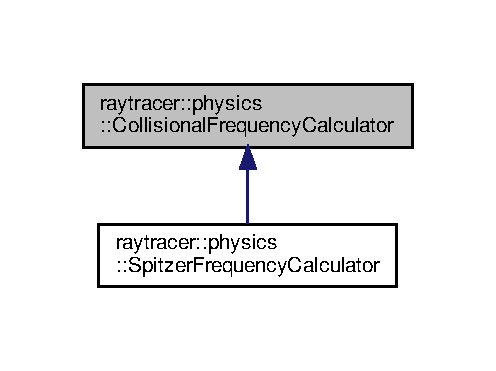
\includegraphics[width=238pt]{classraytracer_1_1physics_1_1CollisionalFrequencyCalculator__inherit__graph}
\end{center}
\end{figure}
\subsection*{Public Member Functions}
\begin{DoxyCompactItemize}
\item 
\mbox{\Hypertarget{classraytracer_1_1physics_1_1CollisionalFrequencyCalculator_ac713b0d5015c3b3efce852894697f1b8}\label{classraytracer_1_1physics_1_1CollisionalFrequencyCalculator_ac713b0d5015c3b3efce852894697f1b8}} 
virtual \hyperlink{structraytracer_1_1physics_1_1Frequency}{Frequency} {\bfseries get\+Collisional\+Frequency} (const \hyperlink{structraytracer_1_1physics_1_1Density}{Density} \&density, const \hyperlink{structraytracer_1_1physics_1_1Temperature}{Temperature} \&temperature, const \hyperlink{structraytracer_1_1physics_1_1Length}{Length} \&laser\+Wavelength, double ionization) const =0
\end{DoxyCompactItemize}


The documentation for this class was generated from the following file\+:\begin{DoxyCompactItemize}
\item 
include/raytracer/physics/Collisional\+Frequency\+Calculators.\+h\end{DoxyCompactItemize}

\hypertarget{classraytracer_1_1physics_1_1ConstantGradientCalculator}{}\section{raytracer\+:\+:physics\+:\+:Constant\+Gradient\+Calculator Class Reference}
\label{classraytracer_1_1physics_1_1ConstantGradientCalculator}\index{raytracer\+::physics\+::\+Constant\+Gradient\+Calculator@{raytracer\+::physics\+::\+Constant\+Gradient\+Calculator}}


\hyperlink{classraytracer_1_1physics_1_1GradientCalculator}{Gradient\+Calculator} that returns a constant Vector no matter what.  




{\ttfamily \#include $<$Gradient\+Calculators.\+h$>$}



Inheritance diagram for raytracer\+:\+:physics\+:\+:Constant\+Gradient\+Calculator\+:\nopagebreak
\begin{figure}[H]
\begin{center}
\leavevmode
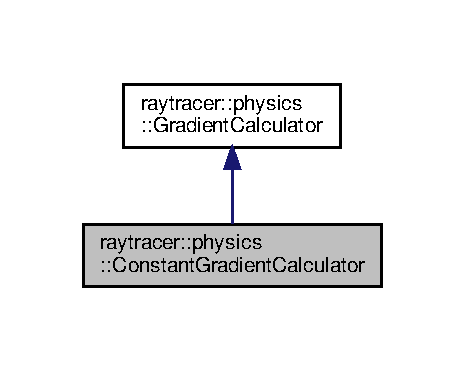
\includegraphics[width=223pt]{classraytracer_1_1physics_1_1ConstantGradientCalculator__inherit__graph}
\end{center}
\end{figure}


Collaboration diagram for raytracer\+:\+:physics\+:\+:Constant\+Gradient\+Calculator\+:\nopagebreak
\begin{figure}[H]
\begin{center}
\leavevmode
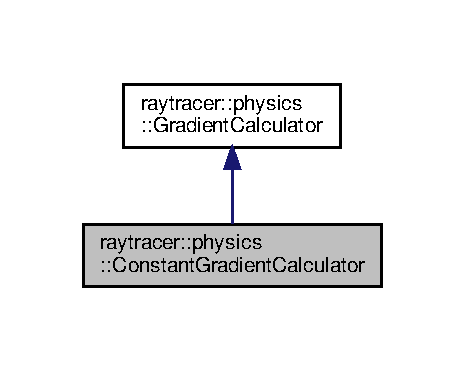
\includegraphics[width=223pt]{classraytracer_1_1physics_1_1ConstantGradientCalculator__coll__graph}
\end{center}
\end{figure}
\subsection*{Public Member Functions}
\begin{DoxyCompactItemize}
\item 
\hyperlink{classraytracer_1_1physics_1_1ConstantGradientCalculator_acf1c99366ffbe215a5150a8ab4c656f5}{Constant\+Gradient\+Calculator} (const \hyperlink{classraytracer_1_1geometry_1_1Vector}{geometry\+::\+Vector} \&gradient)
\begin{DoxyCompactList}\small\item\em Constructor that takes the Vector that will be returned every time as parameter. \end{DoxyCompactList}\item 
\hyperlink{classraytracer_1_1geometry_1_1Vector}{geometry\+::\+Vector} \hyperlink{classraytracer_1_1physics_1_1ConstantGradientCalculator_a62913e68275b1c46893db6fcc74a387f}{get\+Gradient} (const \hyperlink{structraytracer_1_1geometry_1_1Intersection}{geometry\+::\+Intersection} \&) const override
\begin{DoxyCompactList}\small\item\em Returns always the same Vector given at construction. \end{DoxyCompactList}\end{DoxyCompactItemize}


\subsection{Detailed Description}
\hyperlink{classraytracer_1_1physics_1_1GradientCalculator}{Gradient\+Calculator} that returns a constant Vector no matter what. 

\subsection{Constructor \& Destructor Documentation}
\mbox{\Hypertarget{classraytracer_1_1physics_1_1ConstantGradientCalculator_acf1c99366ffbe215a5150a8ab4c656f5}\label{classraytracer_1_1physics_1_1ConstantGradientCalculator_acf1c99366ffbe215a5150a8ab4c656f5}} 
\index{raytracer\+::physics\+::\+Constant\+Gradient\+Calculator@{raytracer\+::physics\+::\+Constant\+Gradient\+Calculator}!Constant\+Gradient\+Calculator@{Constant\+Gradient\+Calculator}}
\index{Constant\+Gradient\+Calculator@{Constant\+Gradient\+Calculator}!raytracer\+::physics\+::\+Constant\+Gradient\+Calculator@{raytracer\+::physics\+::\+Constant\+Gradient\+Calculator}}
\subsubsection{\texorpdfstring{Constant\+Gradient\+Calculator()}{ConstantGradientCalculator()}}
{\footnotesize\ttfamily raytracer\+::physics\+::\+Constant\+Gradient\+Calculator\+::\+Constant\+Gradient\+Calculator (\begin{DoxyParamCaption}\item[{const \hyperlink{classraytracer_1_1geometry_1_1Vector}{geometry\+::\+Vector} \&}]{gradient }\end{DoxyParamCaption})\hspace{0.3cm}{\ttfamily [explicit]}}



Constructor that takes the Vector that will be returned every time as parameter. 


\begin{DoxyParams}{Parameters}
{\em gradient} & -\/ the vector to be returned \\
\hline
\end{DoxyParams}


\subsection{Member Function Documentation}
\mbox{\Hypertarget{classraytracer_1_1physics_1_1ConstantGradientCalculator_a62913e68275b1c46893db6fcc74a387f}\label{classraytracer_1_1physics_1_1ConstantGradientCalculator_a62913e68275b1c46893db6fcc74a387f}} 
\index{raytracer\+::physics\+::\+Constant\+Gradient\+Calculator@{raytracer\+::physics\+::\+Constant\+Gradient\+Calculator}!get\+Gradient@{get\+Gradient}}
\index{get\+Gradient@{get\+Gradient}!raytracer\+::physics\+::\+Constant\+Gradient\+Calculator@{raytracer\+::physics\+::\+Constant\+Gradient\+Calculator}}
\subsubsection{\texorpdfstring{get\+Gradient()}{getGradient()}}
{\footnotesize\ttfamily \hyperlink{classraytracer_1_1geometry_1_1Vector}{geometry\+::\+Vector} raytracer\+::physics\+::\+Constant\+Gradient\+Calculator\+::get\+Gradient (\begin{DoxyParamCaption}\item[{const \hyperlink{structraytracer_1_1geometry_1_1Intersection}{geometry\+::\+Intersection} \&}]{ }\end{DoxyParamCaption}) const\hspace{0.3cm}{\ttfamily [override]}, {\ttfamily [virtual]}}



Returns always the same Vector given at construction. 

\begin{DoxyReturn}{Returns}
vector gradient. 
\end{DoxyReturn}


Implements \hyperlink{classraytracer_1_1physics_1_1GradientCalculator_aeca43f861f5a5099a42bd8af1550f3dc}{raytracer\+::physics\+::\+Gradient\+Calculator}.



The documentation for this class was generated from the following file\+:\begin{DoxyCompactItemize}
\item 
include/raytracer/physics/Gradient\+Calculators.\+h\end{DoxyCompactItemize}

\hypertarget{structraytracer_1_1physics_1_1ContinueStraight}{}\section{raytracer\+:\+:physics\+:\+:Continue\+Straight Struct Reference}
\label{structraytracer_1_1physics_1_1ContinueStraight}\index{raytracer\+::physics\+::\+Continue\+Straight@{raytracer\+::physics\+::\+Continue\+Straight}}


Functor that given an intersection finds next intersection in straight line through intersection.\+next\+Element.  




{\ttfamily \#include $<$Laser\+Propagation.\+h$>$}

\subsection*{Public Member Functions}
\begin{DoxyCompactItemize}
\item 
std\+::unique\+\_\+ptr$<$ \hyperlink{structraytracer_1_1geometry_1_1Intersection}{geometry\+::\+Intersection} $>$ \hyperlink{structraytracer_1_1physics_1_1ContinueStraight_a6b39477b6d24789cc4c98044a556e367}{operator()} (const \hyperlink{structraytracer_1_1geometry_1_1Intersection}{geometry\+::\+Intersection} \&intersection, const \hyperlink{structraytracer_1_1physics_1_1LaserRay}{Laser\+Ray} \&)
\begin{DoxyCompactList}\small\item\em Finds the closest intersection with intersection.\+next\+Element. \end{DoxyCompactList}\end{DoxyCompactItemize}


\subsection{Detailed Description}
Functor that given an intersection finds next intersection in straight line through intersection.\+next\+Element. 

\subsection{Member Function Documentation}
\mbox{\Hypertarget{structraytracer_1_1physics_1_1ContinueStraight_a6b39477b6d24789cc4c98044a556e367}\label{structraytracer_1_1physics_1_1ContinueStraight_a6b39477b6d24789cc4c98044a556e367}} 
\index{raytracer\+::physics\+::\+Continue\+Straight@{raytracer\+::physics\+::\+Continue\+Straight}!operator()@{operator()}}
\index{operator()@{operator()}!raytracer\+::physics\+::\+Continue\+Straight@{raytracer\+::physics\+::\+Continue\+Straight}}
\subsubsection{\texorpdfstring{operator()()}{operator()()}}
{\footnotesize\ttfamily std\+::unique\+\_\+ptr$<$\hyperlink{structraytracer_1_1geometry_1_1Intersection}{geometry\+::\+Intersection}$>$ raytracer\+::physics\+::\+Continue\+Straight\+::operator() (\begin{DoxyParamCaption}\item[{const \hyperlink{structraytracer_1_1geometry_1_1Intersection}{geometry\+::\+Intersection} \&}]{intersection,  }\item[{const \hyperlink{structraytracer_1_1physics_1_1LaserRay}{Laser\+Ray} \&}]{ }\end{DoxyParamCaption})}



Finds the closest intersection with intersection.\+next\+Element. 


\begin{DoxyParams}{Parameters}
{\em intersection} & \\
\hline
\end{DoxyParams}
\begin{DoxyReturn}{Returns}
intersection unique pointer if intersection is found, else it returns nullptr 
\end{DoxyReturn}


The documentation for this struct was generated from the following file\+:\begin{DoxyCompactItemize}
\item 
include/raytracer/physics/Laser\+Propagation.\+h\end{DoxyCompactItemize}

\hypertarget{structraytracer_1_1physics_1_1Density}{}\section{raytracer\+:\+:physics\+:\+:Density Struct Reference}
\label{structraytracer_1_1physics_1_1Density}\index{raytracer\+::physics\+::\+Density@{raytracer\+::physics\+::\+Density}}


Strong type representing length in cm$^\wedge$-\/3.  




{\ttfamily \#include $<$Magnitudes.\+h$>$}



\subsection{Detailed Description}
Strong type representing length in cm$^\wedge$-\/3. 



The documentation for this struct was generated from the following file\+:\begin{DoxyCompactItemize}
\item 
include/raytracer/physics/Magnitudes.\+h\end{DoxyCompactItemize}

\hypertarget{structraytracer_1_1geometry_1_1DiscreteLine}{}\section{raytracer\+:\+:geometry\+:\+:Discrete\+Line Struct Reference}
\label{structraytracer_1_1geometry_1_1DiscreteLine}\index{raytracer\+::geometry\+::\+Discrete\+Line@{raytracer\+::geometry\+::\+Discrete\+Line}}


Structure representing a discretisation of a distance.  




{\ttfamily \#include $<$Mesh.\+h$>$}

\subsection*{Public Attributes}
\begin{DoxyCompactItemize}
\item 
\mbox{\Hypertarget{structraytracer_1_1geometry_1_1DiscreteLine_aea597ae49804ed604f59a1dbcfe577da}\label{structraytracer_1_1geometry_1_1DiscreteLine_aea597ae49804ed604f59a1dbcfe577da}} 
double \hyperlink{structraytracer_1_1geometry_1_1DiscreteLine_aea597ae49804ed604f59a1dbcfe577da}{length}
\begin{DoxyCompactList}\small\item\em Length of the line. \end{DoxyCompactList}\item 
size\+\_\+t \hyperlink{structraytracer_1_1geometry_1_1DiscreteLine_a0657ac3530533ad124a7b6085dfdf928}{segment\+Count}
\begin{DoxyCompactList}\small\item\em Number of segments of the line. \end{DoxyCompactList}\end{DoxyCompactItemize}


\subsection{Detailed Description}
Structure representing a discretisation of a distance. 

That is how many equidistant nodes are on the line with given width. 

\subsection{Member Data Documentation}
\mbox{\Hypertarget{structraytracer_1_1geometry_1_1DiscreteLine_a0657ac3530533ad124a7b6085dfdf928}\label{structraytracer_1_1geometry_1_1DiscreteLine_a0657ac3530533ad124a7b6085dfdf928}} 
\index{raytracer\+::geometry\+::\+Discrete\+Line@{raytracer\+::geometry\+::\+Discrete\+Line}!segment\+Count@{segment\+Count}}
\index{segment\+Count@{segment\+Count}!raytracer\+::geometry\+::\+Discrete\+Line@{raytracer\+::geometry\+::\+Discrete\+Line}}
\subsubsection{\texorpdfstring{segment\+Count}{segmentCount}}
{\footnotesize\ttfamily size\+\_\+t raytracer\+::geometry\+::\+Discrete\+Line\+::segment\+Count}



Number of segments of the line. 

Eg. \hyperlink{structraytracer_1_1geometry_1_1DiscreteLine}{Discrete\+Line} split by four points has three segments. 

The documentation for this struct was generated from the following file\+:\begin{DoxyCompactItemize}
\item 
include/raytracer/geometry/Mesh.\+h\end{DoxyCompactItemize}

\hypertarget{structraytracer_1_1physics_1_1DontStop}{}\section{raytracer\+:\+:physics\+:\+:Dont\+Stop Struct Reference}
\label{structraytracer_1_1physics_1_1DontStop}\index{raytracer\+::physics\+::\+Dont\+Stop@{raytracer\+::physics\+::\+Dont\+Stop}}


Functor for ray propagation that returns false in any case.  




{\ttfamily \#include $<$Laser\+Propagation.\+h$>$}

\subsection*{Public Member Functions}
\begin{DoxyCompactItemize}
\item 
bool \hyperlink{structraytracer_1_1physics_1_1DontStop_a6024e2fafd616c903af29b2ed271568b}{operator()} (const \hyperlink{structraytracer_1_1geometry_1_1Intersection}{geometry\+::\+Intersection} \&, const \hyperlink{structraytracer_1_1physics_1_1LaserRay}{Laser\+Ray} \&)
\begin{DoxyCompactList}\small\item\em Just returns false. \end{DoxyCompactList}\end{DoxyCompactItemize}


\subsection{Detailed Description}
Functor for ray propagation that returns false in any case. 

Convenience struct to keep the call similar to eg. \hyperlink{structraytracer_1_1physics_1_1StopAtCritical}{Stop\+At\+Critical}. 

\subsection{Member Function Documentation}
\mbox{\Hypertarget{structraytracer_1_1physics_1_1DontStop_a6024e2fafd616c903af29b2ed271568b}\label{structraytracer_1_1physics_1_1DontStop_a6024e2fafd616c903af29b2ed271568b}} 
\index{raytracer\+::physics\+::\+Dont\+Stop@{raytracer\+::physics\+::\+Dont\+Stop}!operator()@{operator()}}
\index{operator()@{operator()}!raytracer\+::physics\+::\+Dont\+Stop@{raytracer\+::physics\+::\+Dont\+Stop}}
\subsubsection{\texorpdfstring{operator()()}{operator()()}}
{\footnotesize\ttfamily bool raytracer\+::physics\+::\+Dont\+Stop\+::operator() (\begin{DoxyParamCaption}\item[{const \hyperlink{structraytracer_1_1geometry_1_1Intersection}{geometry\+::\+Intersection} \&}]{,  }\item[{const \hyperlink{structraytracer_1_1physics_1_1LaserRay}{Laser\+Ray} \&}]{ }\end{DoxyParamCaption})}



Just returns false. 

\begin{DoxyReturn}{Returns}
false. 
\end{DoxyReturn}


The documentation for this struct was generated from the following file\+:\begin{DoxyCompactItemize}
\item 
include/raytracer/physics/Laser\+Propagation.\+h\end{DoxyCompactItemize}

\hypertarget{classraytracer_1_1geometry_1_1Element}{}\section{raytracer\+:\+:geometry\+:\+:Element Class Reference}
\label{classraytracer_1_1geometry_1_1Element}\index{raytracer\+::geometry\+::\+Element@{raytracer\+::geometry\+::\+Element}}


Class representing a single volume element in mesh.  




{\ttfamily \#include $<$Element.\+h$>$}

\subsection*{Public Member Functions}
\begin{DoxyCompactItemize}
\item 
const std\+::vector$<$ \hyperlink{classraytracer_1_1geometry_1_1Face}{Face} $\ast$ $>$ \& \hyperlink{classraytracer_1_1geometry_1_1Element_aed405192c2fa9b6488b2be4c78701062}{get\+Faces} () const
\begin{DoxyCompactList}\small\item\em Get the faces of the \hyperlink{classraytracer_1_1geometry_1_1Element}{Element}. \end{DoxyCompactList}\item 
\hyperlink{classraytracer_1_1geometry_1_1Element_a689702f3ea97c81b216759a43cfa1ffe}{Element} (int id, std\+::vector$<$ \hyperlink{classraytracer_1_1geometry_1_1Face}{Face} $\ast$$>$ faces)
\begin{DoxyCompactList}\small\item\em Constructor taking an id and std\+::vector of faces of the element. \end{DoxyCompactList}\item 
int \hyperlink{classraytracer_1_1geometry_1_1Element_ad0780e2bf5e9b3f6918838e9db384e5f}{get\+Id} () const
\begin{DoxyCompactList}\small\item\em Retrieve the id of element. \end{DoxyCompactList}\end{DoxyCompactItemize}


\subsection{Detailed Description}
Class representing a single volume element in mesh. 

Could be any element given by set of faces (edges, surfaces). Instance of this object should not be initialized by user. 

\subsection{Constructor \& Destructor Documentation}
\mbox{\Hypertarget{classraytracer_1_1geometry_1_1Element_a689702f3ea97c81b216759a43cfa1ffe}\label{classraytracer_1_1geometry_1_1Element_a689702f3ea97c81b216759a43cfa1ffe}} 
\index{raytracer\+::geometry\+::\+Element@{raytracer\+::geometry\+::\+Element}!Element@{Element}}
\index{Element@{Element}!raytracer\+::geometry\+::\+Element@{raytracer\+::geometry\+::\+Element}}
\subsubsection{\texorpdfstring{Element()}{Element()}}
{\footnotesize\ttfamily raytracer\+::geometry\+::\+Element\+::\+Element (\begin{DoxyParamCaption}\item[{int}]{id,  }\item[{std\+::vector$<$ \hyperlink{classraytracer_1_1geometry_1_1Face}{Face} $\ast$$>$}]{faces }\end{DoxyParamCaption})\hspace{0.3cm}{\ttfamily [explicit]}}



Constructor taking an id and std\+::vector of faces of the element. 

Clockwise order of faces is preferred in 2D. 
\begin{DoxyParams}{Parameters}
{\em id} & \\
\hline
{\em faces} & \\
\hline
\end{DoxyParams}


\subsection{Member Function Documentation}
\mbox{\Hypertarget{classraytracer_1_1geometry_1_1Element_aed405192c2fa9b6488b2be4c78701062}\label{classraytracer_1_1geometry_1_1Element_aed405192c2fa9b6488b2be4c78701062}} 
\index{raytracer\+::geometry\+::\+Element@{raytracer\+::geometry\+::\+Element}!get\+Faces@{get\+Faces}}
\index{get\+Faces@{get\+Faces}!raytracer\+::geometry\+::\+Element@{raytracer\+::geometry\+::\+Element}}
\subsubsection{\texorpdfstring{get\+Faces()}{getFaces()}}
{\footnotesize\ttfamily const std\+::vector$<$\hyperlink{classraytracer_1_1geometry_1_1Face}{Face} $\ast$$>$\& raytracer\+::geometry\+::\+Element\+::get\+Faces (\begin{DoxyParamCaption}{ }\end{DoxyParamCaption}) const}



Get the faces of the \hyperlink{classraytracer_1_1geometry_1_1Element}{Element}. 

Edges in 2D, surfaces in 3D. \begin{DoxyReturn}{Returns}
the face 
\end{DoxyReturn}
\mbox{\Hypertarget{classraytracer_1_1geometry_1_1Element_ad0780e2bf5e9b3f6918838e9db384e5f}\label{classraytracer_1_1geometry_1_1Element_ad0780e2bf5e9b3f6918838e9db384e5f}} 
\index{raytracer\+::geometry\+::\+Element@{raytracer\+::geometry\+::\+Element}!get\+Id@{get\+Id}}
\index{get\+Id@{get\+Id}!raytracer\+::geometry\+::\+Element@{raytracer\+::geometry\+::\+Element}}
\subsubsection{\texorpdfstring{get\+Id()}{getId()}}
{\footnotesize\ttfamily int raytracer\+::geometry\+::\+Element\+::get\+Id (\begin{DoxyParamCaption}{ }\end{DoxyParamCaption}) const}



Retrieve the id of element. 

\begin{DoxyReturn}{Returns}
id 
\end{DoxyReturn}


The documentation for this class was generated from the following file\+:\begin{DoxyCompactItemize}
\item 
include/raytracer/geometry/Element.\+h\end{DoxyCompactItemize}

\hypertarget{structraytracer_1_1physics_1_1Energy}{}\section{raytracer\+:\+:physics\+:\+:Energy Struct Reference}
\label{structraytracer_1_1physics_1_1Energy}\index{raytracer\+::physics\+::\+Energy@{raytracer\+::physics\+::\+Energy}}


Strong type representing energy in joules.  




{\ttfamily \#include $<$Magnitudes.\+h$>$}



\subsection{Detailed Description}
Strong type representing energy in joules. 



The documentation for this struct was generated from the following file\+:\begin{DoxyCompactItemize}
\item 
include/raytracer/physics/Magnitudes.\+h\end{DoxyCompactItemize}

\hypertarget{classraytracer_1_1geometry_1_1Face}{}\section{raytracer\+:\+:geometry\+:\+:Face Class Reference}
\label{classraytracer_1_1geometry_1_1Face}\index{raytracer\+::geometry\+::\+Face@{raytracer\+::geometry\+::\+Face}}


Class representing a face in mesh (edge in 2D, surface face in 3D).  




{\ttfamily \#include $<$Face.\+h$>$}

\subsection*{Public Member Functions}
\begin{DoxyCompactItemize}
\item 
\hyperlink{classraytracer_1_1geometry_1_1Vector}{Vector} \hyperlink{classraytracer_1_1geometry_1_1Face_aac805c7505f21f9f6bf65c78cdd344de}{get\+Normal} () const
\begin{DoxyCompactList}\small\item\em Calculate a normal to the face (edge in 2D). \end{DoxyCompactList}\item 
const std\+::vector$<$ \hyperlink{classraytracer_1_1geometry_1_1Point}{Point} $\ast$ $>$ \& \hyperlink{classraytracer_1_1geometry_1_1Face_a4cd62fdb7f63bc1acee5fd9a7de233e1}{get\+Points} () const
\begin{DoxyCompactList}\small\item\em Get the points forming the face. \end{DoxyCompactList}\item 
\hyperlink{classraytracer_1_1geometry_1_1Face_ae6c1cac1c9f495b11dfa26cfec783fce}{Face} (int id, std\+::vector$<$ \hyperlink{classraytracer_1_1geometry_1_1Point}{Point} $\ast$$>$ points)
\begin{DoxyCompactList}\small\item\em Construct the face using an id and std\+::vector of points that the face consist of. \end{DoxyCompactList}\item 
const \hyperlink{classraytracer_1_1geometry_1_1Point}{Point} $\ast$ \hyperlink{classraytracer_1_1geometry_1_1Face_a4a71242ce34147b4260d9e62e9a1852c}{is\+Boundary} (const \hyperlink{classraytracer_1_1geometry_1_1Point}{Point} \&point) const
\begin{DoxyCompactList}\small\item\em Return the point on boundary if given point is reasonably close to it. \end{DoxyCompactList}\item 
int \hyperlink{classraytracer_1_1geometry_1_1Face_a83092455149193cca0cfb4e72809e6cf}{get\+Id} () const
\begin{DoxyCompactList}\small\item\em Get the if of the face. \end{DoxyCompactList}\end{DoxyCompactItemize}


\subsection{Detailed Description}
Class representing a face in mesh (edge in 2D, surface face in 3D). 

Instance of this object should not be initialized by user. 

\subsection{Constructor \& Destructor Documentation}
\mbox{\Hypertarget{classraytracer_1_1geometry_1_1Face_ae6c1cac1c9f495b11dfa26cfec783fce}\label{classraytracer_1_1geometry_1_1Face_ae6c1cac1c9f495b11dfa26cfec783fce}} 
\index{raytracer\+::geometry\+::\+Face@{raytracer\+::geometry\+::\+Face}!Face@{Face}}
\index{Face@{Face}!raytracer\+::geometry\+::\+Face@{raytracer\+::geometry\+::\+Face}}
\subsubsection{\texorpdfstring{Face()}{Face()}}
{\footnotesize\ttfamily raytracer\+::geometry\+::\+Face\+::\+Face (\begin{DoxyParamCaption}\item[{int}]{id,  }\item[{std\+::vector$<$ \hyperlink{classraytracer_1_1geometry_1_1Point}{Point} $\ast$$>$}]{points }\end{DoxyParamCaption})\hspace{0.3cm}{\ttfamily [explicit]}}



Construct the face using an id and std\+::vector of points that the face consist of. 


\begin{DoxyParams}{Parameters}
{\em id} & \\
\hline
{\em points} & \\
\hline
\end{DoxyParams}


\subsection{Member Function Documentation}
\mbox{\Hypertarget{classraytracer_1_1geometry_1_1Face_a83092455149193cca0cfb4e72809e6cf}\label{classraytracer_1_1geometry_1_1Face_a83092455149193cca0cfb4e72809e6cf}} 
\index{raytracer\+::geometry\+::\+Face@{raytracer\+::geometry\+::\+Face}!get\+Id@{get\+Id}}
\index{get\+Id@{get\+Id}!raytracer\+::geometry\+::\+Face@{raytracer\+::geometry\+::\+Face}}
\subsubsection{\texorpdfstring{get\+Id()}{getId()}}
{\footnotesize\ttfamily int raytracer\+::geometry\+::\+Face\+::get\+Id (\begin{DoxyParamCaption}{ }\end{DoxyParamCaption}) const}



Get the if of the face. 

\begin{DoxyReturn}{Returns}
id 
\end{DoxyReturn}
\mbox{\Hypertarget{classraytracer_1_1geometry_1_1Face_aac805c7505f21f9f6bf65c78cdd344de}\label{classraytracer_1_1geometry_1_1Face_aac805c7505f21f9f6bf65c78cdd344de}} 
\index{raytracer\+::geometry\+::\+Face@{raytracer\+::geometry\+::\+Face}!get\+Normal@{get\+Normal}}
\index{get\+Normal@{get\+Normal}!raytracer\+::geometry\+::\+Face@{raytracer\+::geometry\+::\+Face}}
\subsubsection{\texorpdfstring{get\+Normal()}{getNormal()}}
{\footnotesize\ttfamily \hyperlink{classraytracer_1_1geometry_1_1Vector}{Vector} raytracer\+::geometry\+::\+Face\+::get\+Normal (\begin{DoxyParamCaption}{ }\end{DoxyParamCaption}) const}



Calculate a normal to the face (edge in 2D). 

By convention in 2D, the normal is outward for points in clockwise order forming a polygon. \begin{DoxyReturn}{Returns}
the normal vector. 
\end{DoxyReturn}
\mbox{\Hypertarget{classraytracer_1_1geometry_1_1Face_a4cd62fdb7f63bc1acee5fd9a7de233e1}\label{classraytracer_1_1geometry_1_1Face_a4cd62fdb7f63bc1acee5fd9a7de233e1}} 
\index{raytracer\+::geometry\+::\+Face@{raytracer\+::geometry\+::\+Face}!get\+Points@{get\+Points}}
\index{get\+Points@{get\+Points}!raytracer\+::geometry\+::\+Face@{raytracer\+::geometry\+::\+Face}}
\subsubsection{\texorpdfstring{get\+Points()}{getPoints()}}
{\footnotesize\ttfamily const std\+::vector$<$\hyperlink{classraytracer_1_1geometry_1_1Point}{Point}$\ast$$>$\& raytracer\+::geometry\+::\+Face\+::get\+Points (\begin{DoxyParamCaption}{ }\end{DoxyParamCaption}) const}



Get the points forming the face. 

\begin{DoxyReturn}{Returns}
the points. 
\end{DoxyReturn}
\mbox{\Hypertarget{classraytracer_1_1geometry_1_1Face_a4a71242ce34147b4260d9e62e9a1852c}\label{classraytracer_1_1geometry_1_1Face_a4a71242ce34147b4260d9e62e9a1852c}} 
\index{raytracer\+::geometry\+::\+Face@{raytracer\+::geometry\+::\+Face}!is\+Boundary@{is\+Boundary}}
\index{is\+Boundary@{is\+Boundary}!raytracer\+::geometry\+::\+Face@{raytracer\+::geometry\+::\+Face}}
\subsubsection{\texorpdfstring{is\+Boundary()}{isBoundary()}}
{\footnotesize\ttfamily const \hyperlink{classraytracer_1_1geometry_1_1Point}{Point}$\ast$ raytracer\+::geometry\+::\+Face\+::is\+Boundary (\begin{DoxyParamCaption}\item[{const \hyperlink{classraytracer_1_1geometry_1_1Point}{Point} \&}]{point }\end{DoxyParamCaption}) const}



Return the point on boundary if given point is reasonably close to it. 


\begin{DoxyParams}{Parameters}
{\em point} & to be compared with all face points \\
\hline
\end{DoxyParams}
\begin{DoxyReturn}{Returns}
on of the face points if it is close to given point. Else it returns nullptr. 
\end{DoxyReturn}


The documentation for this class was generated from the following file\+:\begin{DoxyCompactItemize}
\item 
include/raytracer/geometry/Face.\+h\end{DoxyCompactItemize}

\hypertarget{structraytracer_1_1physics_1_1Frequency}{}\section{raytracer\+:\+:physics\+:\+:Frequency Struct Reference}
\label{structraytracer_1_1physics_1_1Frequency}\index{raytracer\+::physics\+::\+Frequency@{raytracer\+::physics\+::\+Frequency}}


Strong type representing frequency in s$^\wedge$-\/1.  




{\ttfamily \#include $<$Magnitudes.\+h$>$}



\subsection{Detailed Description}
Strong type representing frequency in s$^\wedge$-\/1. 



The documentation for this struct was generated from the following file\+:\begin{DoxyCompactItemize}
\item 
include/raytracer/physics/Magnitudes.\+h\end{DoxyCompactItemize}

\hypertarget{classraytracer_1_1physics_1_1Gaussian}{}\section{raytracer\+:\+:physics\+:\+:Gaussian Class Reference}
\label{classraytracer_1_1physics_1_1Gaussian}\index{raytracer\+::physics\+::\+Gaussian@{raytracer\+::physics\+::\+Gaussian}}


Class representing a 1D gaussian with given parametrs.  




{\ttfamily \#include $<$Math\+Functions.\+h$>$}

\subsection*{Public Member Functions}
\begin{DoxyCompactItemize}
\item 
\hyperlink{classraytracer_1_1physics_1_1Gaussian_a00e90848da44684d9d28cc65e1c2a3dd}{Gaussian} (double F\+W\+HM, double maximum=1, double center=0)
\begin{DoxyCompactList}\small\item\em Construct the gaussian using F\+W\+HM, value at maxim (also the value of the integral) and the center point. \end{DoxyCompactList}\item 
double \hyperlink{classraytracer_1_1physics_1_1Gaussian_a1dfe468b7771b65007f31c9e9c746fce}{operator()} (double x)
\begin{DoxyCompactList}\small\item\em Value of the gaussian at given point x. \end{DoxyCompactList}\end{DoxyCompactItemize}


\subsection{Detailed Description}
Class representing a 1D gaussian with given parametrs. 

\subsection{Constructor \& Destructor Documentation}
\mbox{\Hypertarget{classraytracer_1_1physics_1_1Gaussian_a00e90848da44684d9d28cc65e1c2a3dd}\label{classraytracer_1_1physics_1_1Gaussian_a00e90848da44684d9d28cc65e1c2a3dd}} 
\index{raytracer\+::physics\+::\+Gaussian@{raytracer\+::physics\+::\+Gaussian}!Gaussian@{Gaussian}}
\index{Gaussian@{Gaussian}!raytracer\+::physics\+::\+Gaussian@{raytracer\+::physics\+::\+Gaussian}}
\subsubsection{\texorpdfstring{Gaussian()}{Gaussian()}}
{\footnotesize\ttfamily raytracer\+::physics\+::\+Gaussian\+::\+Gaussian (\begin{DoxyParamCaption}\item[{double}]{F\+W\+HM,  }\item[{double}]{maximum = {\ttfamily 1},  }\item[{double}]{center = {\ttfamily 0} }\end{DoxyParamCaption})\hspace{0.3cm}{\ttfamily [explicit]}}



Construct the gaussian using F\+W\+HM, value at maxim (also the value of the integral) and the center point. 


\begin{DoxyParams}{Parameters}
{\em F\+W\+HM} & \\
\hline
{\em maximum} & or also the intgral value \\
\hline
{\em center} & point \\
\hline
\end{DoxyParams}


\subsection{Member Function Documentation}
\mbox{\Hypertarget{classraytracer_1_1physics_1_1Gaussian_a1dfe468b7771b65007f31c9e9c746fce}\label{classraytracer_1_1physics_1_1Gaussian_a1dfe468b7771b65007f31c9e9c746fce}} 
\index{raytracer\+::physics\+::\+Gaussian@{raytracer\+::physics\+::\+Gaussian}!operator()@{operator()}}
\index{operator()@{operator()}!raytracer\+::physics\+::\+Gaussian@{raytracer\+::physics\+::\+Gaussian}}
\subsubsection{\texorpdfstring{operator()()}{operator()()}}
{\footnotesize\ttfamily double raytracer\+::physics\+::\+Gaussian\+::operator() (\begin{DoxyParamCaption}\item[{double}]{x }\end{DoxyParamCaption})}



Value of the gaussian at given point x. 


\begin{DoxyParams}{Parameters}
{\em x} & \\
\hline
\end{DoxyParams}
\begin{DoxyReturn}{Returns}
the value 
\end{DoxyReturn}


The documentation for this class was generated from the following file\+:\begin{DoxyCompactItemize}
\item 
include/raytracer/physics/Math\+Functions.\+h\end{DoxyCompactItemize}

\hypertarget{classraytracer_1_1physics_1_1GradientCalculator}{}\section{raytracer\+:\+:physics\+:\+:Gradient\+Calculator Class Reference}
\label{classraytracer_1_1physics_1_1GradientCalculator}\index{raytracer\+::physics\+::\+Gradient\+Calculator@{raytracer\+::physics\+::\+Gradient\+Calculator}}


Abstract interface to provide a \hyperlink{classraytracer_1_1physics_1_1GradientCalculator}{Gradient\+Calculator}.  




{\ttfamily \#include $<$Gradient\+Calculators.\+h$>$}



Inheritance diagram for raytracer\+:\+:physics\+:\+:Gradient\+Calculator\+:\nopagebreak
\begin{figure}[H]
\begin{center}
\leavevmode
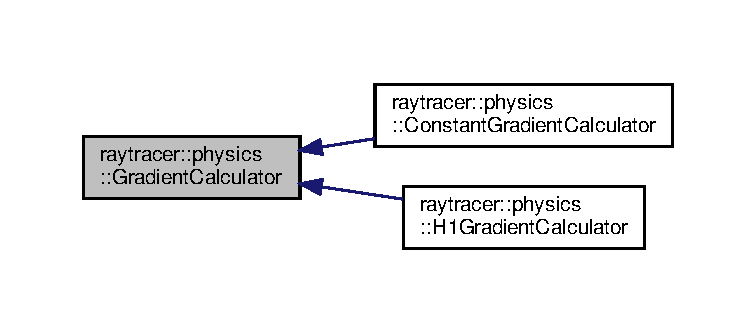
\includegraphics[width=350pt]{classraytracer_1_1physics_1_1GradientCalculator__inherit__graph}
\end{center}
\end{figure}
\subsection*{Public Member Functions}
\begin{DoxyCompactItemize}
\item 
virtual \hyperlink{classraytracer_1_1geometry_1_1Vector}{geometry\+::\+Vector} \hyperlink{classraytracer_1_1physics_1_1GradientCalculator_aeca43f861f5a5099a42bd8af1550f3dc}{get\+Gradient} (const \hyperlink{structraytracer_1_1geometry_1_1Intersection}{geometry\+::\+Intersection} \&) const =0
\begin{DoxyCompactList}\small\item\em Override this. \end{DoxyCompactList}\end{DoxyCompactItemize}


\subsection{Detailed Description}
Abstract interface to provide a \hyperlink{classraytracer_1_1physics_1_1GradientCalculator}{Gradient\+Calculator}. 

To obey this interface implement the get\+Gradient method. 

\subsection{Member Function Documentation}
\mbox{\Hypertarget{classraytracer_1_1physics_1_1GradientCalculator_aeca43f861f5a5099a42bd8af1550f3dc}\label{classraytracer_1_1physics_1_1GradientCalculator_aeca43f861f5a5099a42bd8af1550f3dc}} 
\index{raytracer\+::physics\+::\+Gradient\+Calculator@{raytracer\+::physics\+::\+Gradient\+Calculator}!get\+Gradient@{get\+Gradient}}
\index{get\+Gradient@{get\+Gradient}!raytracer\+::physics\+::\+Gradient\+Calculator@{raytracer\+::physics\+::\+Gradient\+Calculator}}
\subsubsection{\texorpdfstring{get\+Gradient()}{getGradient()}}
{\footnotesize\ttfamily virtual \hyperlink{classraytracer_1_1geometry_1_1Vector}{geometry\+::\+Vector} raytracer\+::physics\+::\+Gradient\+Calculator\+::get\+Gradient (\begin{DoxyParamCaption}\item[{const \hyperlink{structraytracer_1_1geometry_1_1Intersection}{geometry\+::\+Intersection} \&}]{ }\end{DoxyParamCaption}) const\hspace{0.3cm}{\ttfamily [pure virtual]}}



Override this. 

\begin{DoxyReturn}{Returns}
the gradient at given intersection (point). 
\end{DoxyReturn}


Implemented in \hyperlink{classraytracer_1_1physics_1_1H1GradientCalculator_ad1a1647e254efdafb87421d007ca6eb1}{raytracer\+::physics\+::\+H1\+Gradient\+Calculator}, and \hyperlink{classraytracer_1_1physics_1_1ConstantGradientCalculator_a62913e68275b1c46893db6fcc74a387f}{raytracer\+::physics\+::\+Constant\+Gradient\+Calculator}.



The documentation for this class was generated from the following file\+:\begin{DoxyCompactItemize}
\item 
include/raytracer/physics/Gradient\+Calculators.\+h\end{DoxyCompactItemize}

\hypertarget{classraytracer_1_1physics_1_1H1GradientCalculator}{}\section{raytracer\+:\+:physics\+:\+:H1\+Gradient\+Calculator Class Reference}
\label{classraytracer_1_1physics_1_1H1GradientCalculator}\index{raytracer\+::physics\+::\+H1\+Gradient\+Calculator@{raytracer\+::physics\+::\+H1\+Gradient\+Calculator}}


\hyperlink{classraytracer_1_1physics_1_1GradientCalculator}{Gradient\+Calculator} that stores a density grid function defined in H1 space obtained from function given if L2.  




{\ttfamily \#include $<$Gradient\+Calculators.\+h$>$}



Inheritance diagram for raytracer\+:\+:physics\+:\+:H1\+Gradient\+Calculator\+:\nopagebreak
\begin{figure}[H]
\begin{center}
\leavevmode
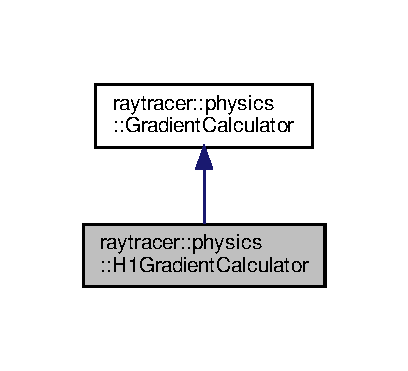
\includegraphics[width=196pt]{classraytracer_1_1physics_1_1H1GradientCalculator__inherit__graph}
\end{center}
\end{figure}


Collaboration diagram for raytracer\+:\+:physics\+:\+:H1\+Gradient\+Calculator\+:\nopagebreak
\begin{figure}[H]
\begin{center}
\leavevmode
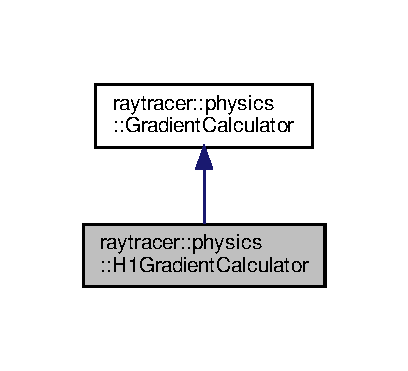
\includegraphics[width=196pt]{classraytracer_1_1physics_1_1H1GradientCalculator__coll__graph}
\end{center}
\end{figure}
\subsection*{Public Member Functions}
\begin{DoxyCompactItemize}
\item 
\hyperlink{classraytracer_1_1physics_1_1H1GradientCalculator_aca95673d4009a25c00eafb913bdb807e}{H1\+Gradient\+Calculator} (mfem\+::\+Finite\+Element\+Space \&l2\+Space, mfem\+::\+Finite\+Element\+Space \&h1\+Space)
\begin{DoxyCompactList}\small\item\em Constructor that expects the l2 and h1 spaces. \end{DoxyCompactList}\item 
\hyperlink{classraytracer_1_1geometry_1_1Vector}{geometry\+::\+Vector} \hyperlink{classraytracer_1_1physics_1_1H1GradientCalculator_ad1a1647e254efdafb87421d007ca6eb1}{get\+Gradient} (const \hyperlink{structraytracer_1_1geometry_1_1Intersection}{geometry\+::\+Intersection} \&intersection) const override
\begin{DoxyCompactList}\small\item\em Return the value of gradient at the intersection point. \end{DoxyCompactList}\item 
void \hyperlink{classraytracer_1_1physics_1_1H1GradientCalculator_a4959559de8b7285f7d6a2c03e5467a35}{update\+Density} (mfem\+::\+Grid\+Function \&density)
\begin{DoxyCompactList}\small\item\em Update the density from which the gradient is calculated. \end{DoxyCompactList}\end{DoxyCompactItemize}


\subsection{Detailed Description}
\hyperlink{classraytracer_1_1physics_1_1GradientCalculator}{Gradient\+Calculator} that stores a density grid function defined in H1 space obtained from function given if L2. 

When get\+Gradient is called the gradient of this function is calculated at given point. 

\subsection{Constructor \& Destructor Documentation}
\mbox{\Hypertarget{classraytracer_1_1physics_1_1H1GradientCalculator_aca95673d4009a25c00eafb913bdb807e}\label{classraytracer_1_1physics_1_1H1GradientCalculator_aca95673d4009a25c00eafb913bdb807e}} 
\index{raytracer\+::physics\+::\+H1\+Gradient\+Calculator@{raytracer\+::physics\+::\+H1\+Gradient\+Calculator}!H1\+Gradient\+Calculator@{H1\+Gradient\+Calculator}}
\index{H1\+Gradient\+Calculator@{H1\+Gradient\+Calculator}!raytracer\+::physics\+::\+H1\+Gradient\+Calculator@{raytracer\+::physics\+::\+H1\+Gradient\+Calculator}}
\subsubsection{\texorpdfstring{H1\+Gradient\+Calculator()}{H1GradientCalculator()}}
{\footnotesize\ttfamily raytracer\+::physics\+::\+H1\+Gradient\+Calculator\+::\+H1\+Gradient\+Calculator (\begin{DoxyParamCaption}\item[{mfem\+::\+Finite\+Element\+Space \&}]{l2\+Space,  }\item[{mfem\+::\+Finite\+Element\+Space \&}]{h1\+Space }\end{DoxyParamCaption})}



Constructor that expects the l2 and h1 spaces. 

L2 is the space in which density is usually defined and H1 is the space into which the density is tranformed to be able to evaluate gradient. 
\begin{DoxyParams}{Parameters}
{\em l2\+Space} & \\
\hline
{\em h1\+Space} & \\
\hline
\end{DoxyParams}


\subsection{Member Function Documentation}
\mbox{\Hypertarget{classraytracer_1_1physics_1_1H1GradientCalculator_ad1a1647e254efdafb87421d007ca6eb1}\label{classraytracer_1_1physics_1_1H1GradientCalculator_ad1a1647e254efdafb87421d007ca6eb1}} 
\index{raytracer\+::physics\+::\+H1\+Gradient\+Calculator@{raytracer\+::physics\+::\+H1\+Gradient\+Calculator}!get\+Gradient@{get\+Gradient}}
\index{get\+Gradient@{get\+Gradient}!raytracer\+::physics\+::\+H1\+Gradient\+Calculator@{raytracer\+::physics\+::\+H1\+Gradient\+Calculator}}
\subsubsection{\texorpdfstring{get\+Gradient()}{getGradient()}}
{\footnotesize\ttfamily \hyperlink{classraytracer_1_1geometry_1_1Vector}{geometry\+::\+Vector} raytracer\+::physics\+::\+H1\+Gradient\+Calculator\+::get\+Gradient (\begin{DoxyParamCaption}\item[{const \hyperlink{structraytracer_1_1geometry_1_1Intersection}{geometry\+::\+Intersection} \&}]{intersection }\end{DoxyParamCaption}) const\hspace{0.3cm}{\ttfamily [override]}, {\ttfamily [virtual]}}



Return the value of gradient at the intersection point. 


\begin{DoxyParams}{Parameters}
{\em intersection} & \\
\hline
\end{DoxyParams}
\begin{DoxyReturn}{Returns}

\end{DoxyReturn}


Implements \hyperlink{classraytracer_1_1physics_1_1GradientCalculator_aeca43f861f5a5099a42bd8af1550f3dc}{raytracer\+::physics\+::\+Gradient\+Calculator}.

\mbox{\Hypertarget{classraytracer_1_1physics_1_1H1GradientCalculator_a4959559de8b7285f7d6a2c03e5467a35}\label{classraytracer_1_1physics_1_1H1GradientCalculator_a4959559de8b7285f7d6a2c03e5467a35}} 
\index{raytracer\+::physics\+::\+H1\+Gradient\+Calculator@{raytracer\+::physics\+::\+H1\+Gradient\+Calculator}!update\+Density@{update\+Density}}
\index{update\+Density@{update\+Density}!raytracer\+::physics\+::\+H1\+Gradient\+Calculator@{raytracer\+::physics\+::\+H1\+Gradient\+Calculator}}
\subsubsection{\texorpdfstring{update\+Density()}{updateDensity()}}
{\footnotesize\ttfamily void raytracer\+::physics\+::\+H1\+Gradient\+Calculator\+::update\+Density (\begin{DoxyParamCaption}\item[{mfem\+::\+Grid\+Function \&}]{density }\end{DoxyParamCaption})}



Update the density from which the gradient is calculated. 

The density should be a function in L2 space. 
\begin{DoxyParams}{Parameters}
{\em density} & defined over L2 \\
\hline
\end{DoxyParams}


The documentation for this class was generated from the following file\+:\begin{DoxyCompactItemize}
\item 
include/raytracer/physics/Gradient\+Calculators.\+h\end{DoxyCompactItemize}

\hypertarget{structraytracer_1_1geometry_1_1HalfLine}{}\section{raytracer\+:\+:geometry\+:\+:Half\+Line Struct Reference}
\label{structraytracer_1_1geometry_1_1HalfLine}\index{raytracer\+::geometry\+::\+Half\+Line@{raytracer\+::geometry\+::\+Half\+Line}}


Structure representing a half line.  




{\ttfamily \#include $<$Geometry\+Functions.\+h$>$}



Collaboration diagram for raytracer\+:\+:geometry\+:\+:Half\+Line\+:\nopagebreak
\begin{figure}[H]
\begin{center}
\leavevmode
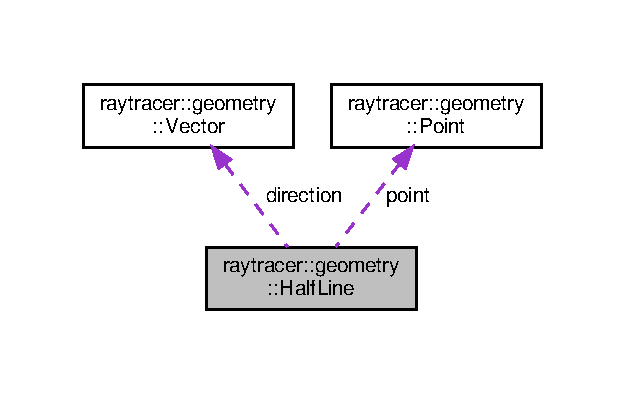
\includegraphics[width=300pt]{structraytracer_1_1geometry_1_1HalfLine__coll__graph}
\end{center}
\end{figure}
\subsection*{Public Attributes}
\begin{DoxyCompactItemize}
\item 
\mbox{\Hypertarget{structraytracer_1_1geometry_1_1HalfLine_a754da5be6d844ecdcd63b8379ff87028}\label{structraytracer_1_1geometry_1_1HalfLine_a754da5be6d844ecdcd63b8379ff87028}} 
\hyperlink{classraytracer_1_1geometry_1_1Point}{Point} \hyperlink{structraytracer_1_1geometry_1_1HalfLine_a754da5be6d844ecdcd63b8379ff87028}{point}
\begin{DoxyCompactList}\small\item\em Origin. \end{DoxyCompactList}\item 
\mbox{\Hypertarget{structraytracer_1_1geometry_1_1HalfLine_a34f254a5bebaf618fee9332c18e9cd11}\label{structraytracer_1_1geometry_1_1HalfLine_a34f254a5bebaf618fee9332c18e9cd11}} 
\hyperlink{classraytracer_1_1geometry_1_1Vector}{Vector} \hyperlink{structraytracer_1_1geometry_1_1HalfLine_a34f254a5bebaf618fee9332c18e9cd11}{direction}
\begin{DoxyCompactList}\small\item\em Direction. \end{DoxyCompactList}\end{DoxyCompactItemize}


\subsection{Detailed Description}
Structure representing a half line. 

It originates from a point and has a direction. 

The documentation for this struct was generated from the following file\+:\begin{DoxyCompactItemize}
\item 
include/raytracer/geometry/Geometry\+Functions.\+h\end{DoxyCompactItemize}

\hypertarget{structraytracer_1_1geometry_1_1Intersection}{}\section{raytracer\+:\+:geometry\+:\+:Intersection Struct Reference}
\label{structraytracer_1_1geometry_1_1Intersection}\index{raytracer\+::geometry\+::\+Intersection@{raytracer\+::geometry\+::\+Intersection}}


Structure representing a single intersection of \hyperlink{structraytracer_1_1geometry_1_1HalfLine}{Half\+Line} with a mesh.  




{\ttfamily \#include $<$Geometry\+Functions.\+h$>$}



Collaboration diagram for raytracer\+:\+:geometry\+:\+:Intersection\+:\nopagebreak
\begin{figure}[H]
\begin{center}
\leavevmode
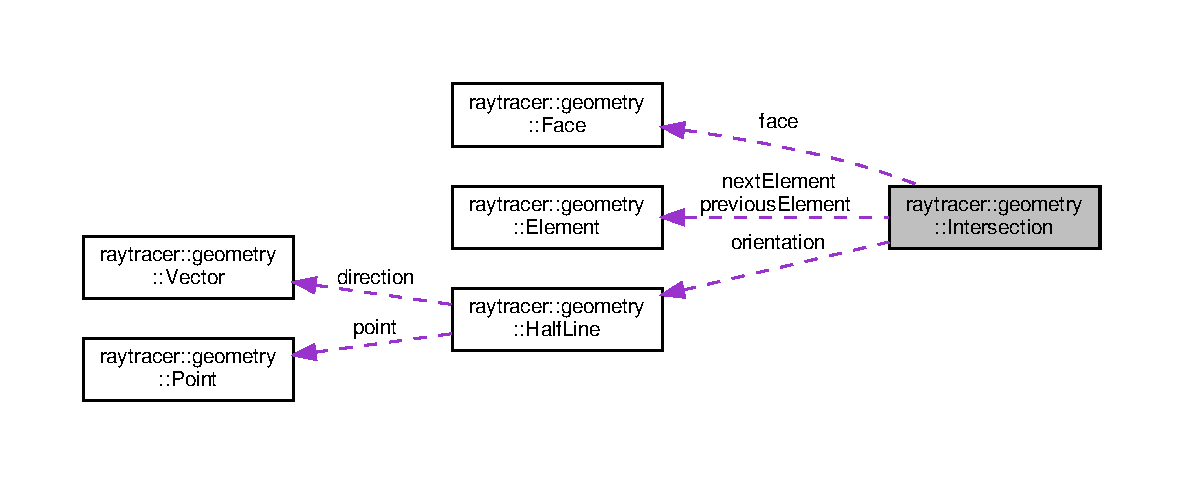
\includegraphics[width=350pt]{structraytracer_1_1geometry_1_1Intersection__coll__graph}
\end{center}
\end{figure}
\subsection*{Public Attributes}
\begin{DoxyCompactItemize}
\item 
\hyperlink{structraytracer_1_1geometry_1_1HalfLine}{Half\+Line} \hyperlink{structraytracer_1_1geometry_1_1Intersection_ac899194bf216a03b025f61b1981c8ce7}{orientation} \{\}
\begin{DoxyCompactList}\small\item\em Orientation is represented by \hyperlink{structraytracer_1_1geometry_1_1HalfLine}{Half\+Line}. \end{DoxyCompactList}\item 
const \hyperlink{classraytracer_1_1geometry_1_1Face}{Face} $\ast$ \hyperlink{structraytracer_1_1geometry_1_1Intersection_a993ca640c2f62bead2d29ebd2d605dc4}{face} \{\}
\begin{DoxyCompactList}\small\item\em Pointer to the \hyperlink{classraytracer_1_1geometry_1_1Face}{Face} that was intersected by the ray. \end{DoxyCompactList}\item 
const \hyperlink{classraytracer_1_1geometry_1_1Element}{Element} $\ast$ \hyperlink{structraytracer_1_1geometry_1_1Intersection_a141dc9291977b52dc561e1dff86694d9}{next\+Element} \{\}
\begin{DoxyCompactList}\small\item\em Pointer to the next \hyperlink{classraytracer_1_1geometry_1_1Element}{Element} that the ray would go to from the \hyperlink{classraytracer_1_1geometry_1_1Face}{Face}. \end{DoxyCompactList}\item 
const \hyperlink{classraytracer_1_1geometry_1_1Element}{Element} $\ast$ \hyperlink{structraytracer_1_1geometry_1_1Intersection_a22c5bb7b48818d87ff42cd426d5ac910}{previous\+Element} \{\}
\begin{DoxyCompactList}\small\item\em Pointer to the previous \hyperlink{classraytracer_1_1geometry_1_1Element}{Element} that the ray actually came from. \end{DoxyCompactList}\end{DoxyCompactItemize}


\subsection{Detailed Description}
Structure representing a single intersection of \hyperlink{structraytracer_1_1geometry_1_1HalfLine}{Half\+Line} with a mesh. 

\subsection{Member Data Documentation}
\mbox{\Hypertarget{structraytracer_1_1geometry_1_1Intersection_a993ca640c2f62bead2d29ebd2d605dc4}\label{structraytracer_1_1geometry_1_1Intersection_a993ca640c2f62bead2d29ebd2d605dc4}} 
\index{raytracer\+::geometry\+::\+Intersection@{raytracer\+::geometry\+::\+Intersection}!face@{face}}
\index{face@{face}!raytracer\+::geometry\+::\+Intersection@{raytracer\+::geometry\+::\+Intersection}}
\subsubsection{\texorpdfstring{face}{face}}
{\footnotesize\ttfamily const \hyperlink{classraytracer_1_1geometry_1_1Face}{Face}$\ast$ raytracer\+::geometry\+::\+Intersection\+::face \{\}}



Pointer to the \hyperlink{classraytracer_1_1geometry_1_1Face}{Face} that was intersected by the ray. 

\mbox{\Hypertarget{structraytracer_1_1geometry_1_1Intersection_a141dc9291977b52dc561e1dff86694d9}\label{structraytracer_1_1geometry_1_1Intersection_a141dc9291977b52dc561e1dff86694d9}} 
\index{raytracer\+::geometry\+::\+Intersection@{raytracer\+::geometry\+::\+Intersection}!next\+Element@{next\+Element}}
\index{next\+Element@{next\+Element}!raytracer\+::geometry\+::\+Intersection@{raytracer\+::geometry\+::\+Intersection}}
\subsubsection{\texorpdfstring{next\+Element}{nextElement}}
{\footnotesize\ttfamily const \hyperlink{classraytracer_1_1geometry_1_1Element}{Element}$\ast$ raytracer\+::geometry\+::\+Intersection\+::next\+Element \{\}}



Pointer to the next \hyperlink{classraytracer_1_1geometry_1_1Element}{Element} that the ray would go to from the \hyperlink{classraytracer_1_1geometry_1_1Face}{Face}. 

Could be null if the ray just left the \hyperlink{classraytracer_1_1geometry_1_1Mesh}{Mesh}. \mbox{\Hypertarget{structraytracer_1_1geometry_1_1Intersection_ac899194bf216a03b025f61b1981c8ce7}\label{structraytracer_1_1geometry_1_1Intersection_ac899194bf216a03b025f61b1981c8ce7}} 
\index{raytracer\+::geometry\+::\+Intersection@{raytracer\+::geometry\+::\+Intersection}!orientation@{orientation}}
\index{orientation@{orientation}!raytracer\+::geometry\+::\+Intersection@{raytracer\+::geometry\+::\+Intersection}}
\subsubsection{\texorpdfstring{orientation}{orientation}}
{\footnotesize\ttfamily \hyperlink{structraytracer_1_1geometry_1_1HalfLine}{Half\+Line} raytracer\+::geometry\+::\+Intersection\+::orientation \{\}}



Orientation is represented by \hyperlink{structraytracer_1_1geometry_1_1HalfLine}{Half\+Line}. 

The origin of the \hyperlink{structraytracer_1_1geometry_1_1HalfLine}{Half\+Line} is the intersection point. The direction of the \hyperlink{structraytracer_1_1geometry_1_1HalfLine}{Half\+Line} is the direction the ray had when it intersected the \hyperlink{classraytracer_1_1geometry_1_1Mesh}{Mesh}. \mbox{\Hypertarget{structraytracer_1_1geometry_1_1Intersection_a22c5bb7b48818d87ff42cd426d5ac910}\label{structraytracer_1_1geometry_1_1Intersection_a22c5bb7b48818d87ff42cd426d5ac910}} 
\index{raytracer\+::geometry\+::\+Intersection@{raytracer\+::geometry\+::\+Intersection}!previous\+Element@{previous\+Element}}
\index{previous\+Element@{previous\+Element}!raytracer\+::geometry\+::\+Intersection@{raytracer\+::geometry\+::\+Intersection}}
\subsubsection{\texorpdfstring{previous\+Element}{previousElement}}
{\footnotesize\ttfamily const \hyperlink{classraytracer_1_1geometry_1_1Element}{Element}$\ast$ raytracer\+::geometry\+::\+Intersection\+::previous\+Element \{\}}



Pointer to the previous \hyperlink{classraytracer_1_1geometry_1_1Element}{Element} that the ray actually came from. 

could be null if the ray just entered the \hyperlink{classraytracer_1_1geometry_1_1Mesh}{Mesh}. 

The documentation for this struct was generated from the following file\+:\begin{DoxyCompactItemize}
\item 
include/raytracer/geometry/Geometry\+Functions.\+h\end{DoxyCompactItemize}

\hypertarget{classraytracer_1_1physics_1_1Laser}{}\section{raytracer\+:\+:physics\+:\+:Laser Class Reference}
\label{classraytracer_1_1physics_1_1Laser}\index{raytracer\+::physics\+::\+Laser@{raytracer\+::physics\+::\+Laser}}


Class representing a real physical laser.  




{\ttfamily \#include $<$Laser.\+h$>$}

\subsection*{Public Member Functions}
\begin{DoxyCompactItemize}
\item 
\hyperlink{classraytracer_1_1physics_1_1Laser_aaac32df0c929962080aa6c6e0acdff17}{Laser} (\hyperlink{structraytracer_1_1physics_1_1Length}{Length} wavelength, Direction\+Fun direction\+Function, Energy\+Fun energy\+Function, \hyperlink{classraytracer_1_1geometry_1_1Point}{geometry\+::\+Point} start\+Point, \hyperlink{classraytracer_1_1geometry_1_1Point}{geometry\+::\+Point} end\+Point)
\begin{DoxyCompactList}\small\item\em Construct it using the wavelength in cm, direction\+Function, energy\+Function and two points in space between which the laser originates. \end{DoxyCompactList}\item 
void \hyperlink{classraytracer_1_1physics_1_1Laser_a5f2620bcf974198ccc541ea60a7ed6a9}{generate\+Rays} (size\+\_\+t count)
\begin{DoxyCompactList}\small\item\em Generate a set of equidistant Laser\+Rays given by the parameters of the whole laser. \end{DoxyCompactList}\item 
const std\+::vector$<$ \hyperlink{structraytracer_1_1physics_1_1LaserRay}{Laser\+Ray} $>$ \& \hyperlink{classraytracer_1_1physics_1_1Laser_af35cc781f5f6b39bfa9e25369a63a856}{get\+Rays} () const
\begin{DoxyCompactList}\small\item\em Get all the rays in that are in the current state of \hyperlink{classraytracer_1_1physics_1_1Laser}{Laser}. \end{DoxyCompactList}\item 
{\footnotesize template$<$typename Inters\+Func , typename Stop\+Condition $>$ }\\void \hyperlink{classraytracer_1_1physics_1_1Laser_a6e8478566acd96cb5a752f236cd070f3}{generate\+Intersections} (const \hyperlink{classraytracer_1_1geometry_1_1Mesh}{geometry\+::\+Mesh} \&mesh, Inters\+Func find\+Inters, Stop\+Condition stop\+Condition)
\begin{DoxyCompactList}\small\item\em If there are any rays in \hyperlink{classraytracer_1_1physics_1_1Laser}{Laser} theit intersections with given mesh will be found. \end{DoxyCompactList}\item 
void \hyperlink{classraytracer_1_1physics_1_1Laser_adfb22ae48261bdc37db1f36fca20065f}{save\+Rays\+To\+Json} (const std\+::string \&filename)
\begin{DoxyCompactList}\small\item\em Save all the rays to a file in J\+S\+ON format. \end{DoxyCompactList}\end{DoxyCompactItemize}


\subsection{Detailed Description}
Class representing a real physical laser. 

It is given by its origin, and energy. 

\subsection{Constructor \& Destructor Documentation}
\mbox{\Hypertarget{classraytracer_1_1physics_1_1Laser_aaac32df0c929962080aa6c6e0acdff17}\label{classraytracer_1_1physics_1_1Laser_aaac32df0c929962080aa6c6e0acdff17}} 
\index{raytracer\+::physics\+::\+Laser@{raytracer\+::physics\+::\+Laser}!Laser@{Laser}}
\index{Laser@{Laser}!raytracer\+::physics\+::\+Laser@{raytracer\+::physics\+::\+Laser}}
\subsubsection{\texorpdfstring{Laser()}{Laser()}}
{\footnotesize\ttfamily raytracer\+::physics\+::\+Laser\+::\+Laser (\begin{DoxyParamCaption}\item[{\hyperlink{structraytracer_1_1physics_1_1Length}{Length}}]{wavelength,  }\item[{Direction\+Fun}]{direction\+Function,  }\item[{Energy\+Fun}]{energy\+Function,  }\item[{\hyperlink{classraytracer_1_1geometry_1_1Point}{geometry\+::\+Point}}]{start\+Point,  }\item[{\hyperlink{classraytracer_1_1geometry_1_1Point}{geometry\+::\+Point}}]{end\+Point }\end{DoxyParamCaption})}



Construct it using the wavelength in cm, direction\+Function, energy\+Function and two points in space between which the laser originates. 

The direction\+Function should return the direction of the laser given an arbitrary point in space. The energy function should return the energy of the laser base on the parameter x. X is expected to be meassured from the center of the laser.


\begin{DoxyParams}{Parameters}
{\em wavelength} & of the laser in cm \\
\hline
{\em direction\+Function} & function with signature (const Point\& point) -\/$>$ Vector \\
\hline
{\em energy\+Function} & function with signature (double x) -\/$>$ double. \\
\hline
{\em start\+Point} & from which to start the generation of the rays \\
\hline
{\em end\+Point} & where to end the generation of the points \\
\hline
\end{DoxyParams}


\subsection{Member Function Documentation}
\mbox{\Hypertarget{classraytracer_1_1physics_1_1Laser_a6e8478566acd96cb5a752f236cd070f3}\label{classraytracer_1_1physics_1_1Laser_a6e8478566acd96cb5a752f236cd070f3}} 
\index{raytracer\+::physics\+::\+Laser@{raytracer\+::physics\+::\+Laser}!generate\+Intersections@{generate\+Intersections}}
\index{generate\+Intersections@{generate\+Intersections}!raytracer\+::physics\+::\+Laser@{raytracer\+::physics\+::\+Laser}}
\subsubsection{\texorpdfstring{generate\+Intersections()}{generateIntersections()}}
{\footnotesize\ttfamily template$<$typename Inters\+Func , typename Stop\+Condition $>$ \\
void raytracer\+::physics\+::\+Laser\+::generate\+Intersections (\begin{DoxyParamCaption}\item[{const \hyperlink{classraytracer_1_1geometry_1_1Mesh}{geometry\+::\+Mesh} \&}]{mesh,  }\item[{Inters\+Func}]{find\+Inters,  }\item[{Stop\+Condition}]{stop\+Condition }\end{DoxyParamCaption})\hspace{0.3cm}{\ttfamily [inline]}}



If there are any rays in \hyperlink{classraytracer_1_1physics_1_1Laser}{Laser} theit intersections with given mesh will be found. 

This just calls \hyperlink{structraytracer_1_1physics_1_1LaserRay_ab54b08958f38711dfd46d49bb2ef583d}{Laser\+Ray\+::generate\+Intersections} for each of the rays. 
\begin{DoxyTemplParams}{Template Parameters}
{\em Inters\+Func} & function with signature (Intersection, \hyperlink{structraytracer_1_1physics_1_1LaserRay}{Laser\+Ray}) -\/$>$ std\+::unique\+\_\+ptr$<$\+Intersection$>$ \\
\hline
{\em Stop\+Condition} & function with signature (Intersection, \hyperlink{structraytracer_1_1physics_1_1LaserRay}{Laser\+Ray}) -\/$>$ bool \\
\hline
\end{DoxyTemplParams}

\begin{DoxyParams}{Parameters}
{\em mesh} & to be intersected \\
\hline
{\em find\+Inters} & is propagated to \hyperlink{structraytracer_1_1physics_1_1LaserRay_ab54b08958f38711dfd46d49bb2ef583d}{Laser\+Ray\+::generate\+Intersections} with additional parameter being the laser\+Ray \\
\hline
{\em stop\+Condition} & is propagated to \hyperlink{structraytracer_1_1physics_1_1LaserRay_ab54b08958f38711dfd46d49bb2ef583d}{Laser\+Ray\+::generate\+Intersections} with additional parameter being the laser\+Ray \\
\hline
\end{DoxyParams}
\mbox{\Hypertarget{classraytracer_1_1physics_1_1Laser_a5f2620bcf974198ccc541ea60a7ed6a9}\label{classraytracer_1_1physics_1_1Laser_a5f2620bcf974198ccc541ea60a7ed6a9}} 
\index{raytracer\+::physics\+::\+Laser@{raytracer\+::physics\+::\+Laser}!generate\+Rays@{generate\+Rays}}
\index{generate\+Rays@{generate\+Rays}!raytracer\+::physics\+::\+Laser@{raytracer\+::physics\+::\+Laser}}
\subsubsection{\texorpdfstring{generate\+Rays()}{generateRays()}}
{\footnotesize\ttfamily void raytracer\+::physics\+::\+Laser\+::generate\+Rays (\begin{DoxyParamCaption}\item[{size\+\_\+t}]{count }\end{DoxyParamCaption})}



Generate a set of equidistant Laser\+Rays given by the parameters of the whole laser. 

The rays are generated originating from an edge between a start and end points of the laser. These will be set to the this \hyperlink{classraytracer_1_1physics_1_1Laser}{Laser} state.


\begin{DoxyParams}{Parameters}
{\em count} & number of rays to be generated \\
\hline
\end{DoxyParams}
\begin{DoxyReturn}{Returns}
a sequence of rays 
\end{DoxyReturn}
\mbox{\Hypertarget{classraytracer_1_1physics_1_1Laser_af35cc781f5f6b39bfa9e25369a63a856}\label{classraytracer_1_1physics_1_1Laser_af35cc781f5f6b39bfa9e25369a63a856}} 
\index{raytracer\+::physics\+::\+Laser@{raytracer\+::physics\+::\+Laser}!get\+Rays@{get\+Rays}}
\index{get\+Rays@{get\+Rays}!raytracer\+::physics\+::\+Laser@{raytracer\+::physics\+::\+Laser}}
\subsubsection{\texorpdfstring{get\+Rays()}{getRays()}}
{\footnotesize\ttfamily const std\+::vector$<$\hyperlink{structraytracer_1_1physics_1_1LaserRay}{Laser\+Ray}$>$\& raytracer\+::physics\+::\+Laser\+::get\+Rays (\begin{DoxyParamCaption}{ }\end{DoxyParamCaption}) const}



Get all the rays in that are in the current state of \hyperlink{classraytracer_1_1physics_1_1Laser}{Laser}. 

\begin{DoxyReturn}{Returns}
all rays 
\end{DoxyReturn}
\mbox{\Hypertarget{classraytracer_1_1physics_1_1Laser_adfb22ae48261bdc37db1f36fca20065f}\label{classraytracer_1_1physics_1_1Laser_adfb22ae48261bdc37db1f36fca20065f}} 
\index{raytracer\+::physics\+::\+Laser@{raytracer\+::physics\+::\+Laser}!save\+Rays\+To\+Json@{save\+Rays\+To\+Json}}
\index{save\+Rays\+To\+Json@{save\+Rays\+To\+Json}!raytracer\+::physics\+::\+Laser@{raytracer\+::physics\+::\+Laser}}
\subsubsection{\texorpdfstring{save\+Rays\+To\+Json()}{saveRaysToJson()}}
{\footnotesize\ttfamily void raytracer\+::physics\+::\+Laser\+::save\+Rays\+To\+Json (\begin{DoxyParamCaption}\item[{const std\+::string \&}]{filename }\end{DoxyParamCaption})}



Save all the rays to a file in J\+S\+ON format. 

There will be one object called rays. It is an array of rays each beeing a sequence of points eg. \mbox{[}0, 1\mbox{]} 
\begin{DoxyParams}{Parameters}
{\em filename} & name of the json file including extension \\
\hline
\end{DoxyParams}


The documentation for this class was generated from the following file\+:\begin{DoxyCompactItemize}
\item 
include/raytracer/physics/Laser.\+h\end{DoxyCompactItemize}

\hypertarget{structraytracer_1_1physics_1_1LaserRay}{}\section{raytracer\+:\+:physics\+:\+:Laser\+Ray Struct Reference}
\label{structraytracer_1_1physics_1_1LaserRay}\index{raytracer\+::physics\+::\+Laser\+Ray@{raytracer\+::physics\+::\+Laser\+Ray}}


Structure representing a single \hyperlink{structraytracer_1_1physics_1_1LaserRay}{Laser\+Ray}.  




{\ttfamily \#include $<$Laser\+Ray.\+h$>$}



Collaboration diagram for raytracer\+:\+:physics\+:\+:Laser\+Ray\+:\nopagebreak
\begin{figure}[H]
\begin{center}
\leavevmode
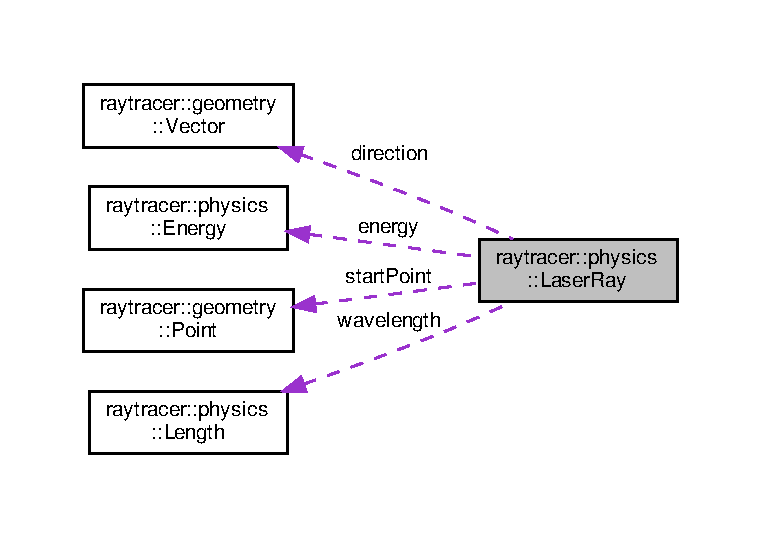
\includegraphics[width=350pt]{structraytracer_1_1physics_1_1LaserRay__coll__graph}
\end{center}
\end{figure}
\subsection*{Public Member Functions}
\begin{DoxyCompactItemize}
\item 
\mbox{\Hypertarget{structraytracer_1_1physics_1_1LaserRay_abd3a438ada8ed1b8c8c6a67507fa99e1}\label{structraytracer_1_1physics_1_1LaserRay_abd3a438ada8ed1b8c8c6a67507fa99e1}} 
\hyperlink{structraytracer_1_1physics_1_1Density}{Density} \hyperlink{structraytracer_1_1physics_1_1LaserRay_abd3a438ada8ed1b8c8c6a67507fa99e1}{get\+Critical\+Density} () const
\begin{DoxyCompactList}\small\item\em The electron critical density of the \hyperlink{structraytracer_1_1physics_1_1LaserRay}{Laser\+Ray}. \end{DoxyCompactList}\item 
double \hyperlink{structraytracer_1_1physics_1_1LaserRay_ae17f1eba8f0f91cb5960a865aacb9849}{get\+Refractive\+Index} (const \hyperlink{structraytracer_1_1physics_1_1Density}{Density} \&density, const \hyperlink{structraytracer_1_1physics_1_1Frequency}{Frequency} \&collision\+Frequency) const
\begin{DoxyCompactList}\small\item\em Calculate the index of refraction based on current density, collisional frequency. \end{DoxyCompactList}\item 
double \hyperlink{structraytracer_1_1physics_1_1LaserRay_adaba8f65ba15512c6022f5eb55a3a41a}{get\+Inverse\+Bremsstrahlung\+Coeff} (const \hyperlink{structraytracer_1_1physics_1_1Density}{Density} \&density, const \hyperlink{structraytracer_1_1physics_1_1Frequency}{Frequency} \&collision\+Frequency) const
\begin{DoxyCompactList}\small\item\em Calculate the inverse bremsstrahlung coefficient base on current density and collisional frequency. \end{DoxyCompactList}\item 
std\+::complex$<$ double $>$ \hyperlink{structraytracer_1_1physics_1_1LaserRay_a2a033aeed48df8c008c221545e7a93a2}{get\+Permittivity} (const \hyperlink{structraytracer_1_1physics_1_1Density}{Density} \&density, const \hyperlink{structraytracer_1_1physics_1_1Frequency}{Frequency} \&collision\+Frequency) const
\begin{DoxyCompactList}\small\item\em Calculate the permittivity based on current density and collision\+Frequency. \end{DoxyCompactList}\item 
{\footnotesize template$<$typename Inters\+Func , typename Stop\+Condition $>$ }\\void \hyperlink{structraytracer_1_1physics_1_1LaserRay_ab54b08958f38711dfd46d49bb2ef583d}{generate\+Intersections} (const \hyperlink{classraytracer_1_1geometry_1_1Mesh}{geometry\+::\+Mesh} \&mesh, Inters\+Func find\+Inters, Stop\+Condition stop\+Condition)
\begin{DoxyCompactList}\small\item\em Wrapper around Ray\+::find\+Intersections. \end{DoxyCompactList}\end{DoxyCompactItemize}
\subsection*{Public Attributes}
\begin{DoxyCompactItemize}
\item 
\hyperlink{classraytracer_1_1geometry_1_1Point}{geometry\+::\+Point} \hyperlink{structraytracer_1_1physics_1_1LaserRay_a7d81914ce19108013d4cd1dcf8c62216}{start\+Point} \{\}
\begin{DoxyCompactList}\small\item\em The point from which the \hyperlink{structraytracer_1_1physics_1_1LaserRay}{Laser\+Ray} originates. \end{DoxyCompactList}\item 
\hyperlink{classraytracer_1_1geometry_1_1Vector}{geometry\+::\+Vector} \hyperlink{structraytracer_1_1physics_1_1LaserRay_a9244628df4215dc86dcbe134c847e54d}{direction} \{\}
\begin{DoxyCompactList}\small\item\em The initial direction of the \hyperlink{structraytracer_1_1physics_1_1LaserRay}{Laser\+Ray}. \end{DoxyCompactList}\item 
\hyperlink{structraytracer_1_1physics_1_1Energy}{Energy} \hyperlink{structraytracer_1_1physics_1_1LaserRay_aed5483243c44e1a7535b249afae7b1ad}{energy} \{\}
\begin{DoxyCompactList}\small\item\em Absolute energy carried by the \hyperlink{structraytracer_1_1physics_1_1LaserRay}{Laser\+Ray}. \end{DoxyCompactList}\item 
\mbox{\Hypertarget{structraytracer_1_1physics_1_1LaserRay_af0d865a3db62a989276cad5dbd2d28cd}\label{structraytracer_1_1physics_1_1LaserRay_af0d865a3db62a989276cad5dbd2d28cd}} 
\hyperlink{structraytracer_1_1physics_1_1Length}{Length} \hyperlink{structraytracer_1_1physics_1_1LaserRay_af0d865a3db62a989276cad5dbd2d28cd}{wavelength} \{\}
\begin{DoxyCompactList}\small\item\em Wavelength of the \hyperlink{structraytracer_1_1physics_1_1LaserRay}{Laser\+Ray} in cm. \end{DoxyCompactList}\item 
std\+::vector$<$ \hyperlink{structraytracer_1_1geometry_1_1Intersection}{geometry\+::\+Intersection} $>$ \hyperlink{structraytracer_1_1physics_1_1LaserRay_a8d41ff2d7ea5212bd39d1c4ae8ffde7d}{intersections}
\begin{DoxyCompactList}\small\item\em Sequence of all intersections with given Mesh. \end{DoxyCompactList}\end{DoxyCompactItemize}


\subsection{Detailed Description}
Structure representing a single \hyperlink{structraytracer_1_1physics_1_1LaserRay}{Laser\+Ray}. 

It has associated energy but no width for now. 

\subsection{Member Function Documentation}
\mbox{\Hypertarget{structraytracer_1_1physics_1_1LaserRay_ab54b08958f38711dfd46d49bb2ef583d}\label{structraytracer_1_1physics_1_1LaserRay_ab54b08958f38711dfd46d49bb2ef583d}} 
\index{raytracer\+::physics\+::\+Laser\+Ray@{raytracer\+::physics\+::\+Laser\+Ray}!generate\+Intersections@{generate\+Intersections}}
\index{generate\+Intersections@{generate\+Intersections}!raytracer\+::physics\+::\+Laser\+Ray@{raytracer\+::physics\+::\+Laser\+Ray}}
\subsubsection{\texorpdfstring{generate\+Intersections()}{generateIntersections()}}
{\footnotesize\ttfamily template$<$typename Inters\+Func , typename Stop\+Condition $>$ \\
void raytracer\+::physics\+::\+Laser\+Ray\+::generate\+Intersections (\begin{DoxyParamCaption}\item[{const \hyperlink{classraytracer_1_1geometry_1_1Mesh}{geometry\+::\+Mesh} \&}]{mesh,  }\item[{Inters\+Func}]{find\+Inters,  }\item[{Stop\+Condition}]{stop\+Condition }\end{DoxyParamCaption})\hspace{0.3cm}{\ttfamily [inline]}}



Wrapper around Ray\+::find\+Intersections. 

It generates a ray based on the \hyperlink{structraytracer_1_1physics_1_1LaserRay}{Laser\+Ray} properties and saves the result to \hyperlink{structraytracer_1_1physics_1_1LaserRay_a8d41ff2d7ea5212bd39d1c4ae8ffde7d}{Laser\+Ray\+::intersections}.


\begin{DoxyTemplParams}{Template Parameters}
{\em Inters\+Func} & function with signature (Intersection) -\/$>$ std\+::unique\+\_\+ptr$<$\+Intersection$>$ \\
\hline
{\em Stop\+Condition} & function with signature (Intersection) -\/$>$ bool \\
\hline
\end{DoxyTemplParams}

\begin{DoxyParams}{Parameters}
{\em mesh} & to be intersected \\
\hline
{\em find\+Inters} & will be propagated to Ray\+::find\+Intersections as is. \\
\hline
{\em stop\+Condition} & will be propagated to ray\+::find\+Intersections as is. \\
\hline
\end{DoxyParams}
\mbox{\Hypertarget{structraytracer_1_1physics_1_1LaserRay_adaba8f65ba15512c6022f5eb55a3a41a}\label{structraytracer_1_1physics_1_1LaserRay_adaba8f65ba15512c6022f5eb55a3a41a}} 
\index{raytracer\+::physics\+::\+Laser\+Ray@{raytracer\+::physics\+::\+Laser\+Ray}!get\+Inverse\+Bremsstrahlung\+Coeff@{get\+Inverse\+Bremsstrahlung\+Coeff}}
\index{get\+Inverse\+Bremsstrahlung\+Coeff@{get\+Inverse\+Bremsstrahlung\+Coeff}!raytracer\+::physics\+::\+Laser\+Ray@{raytracer\+::physics\+::\+Laser\+Ray}}
\subsubsection{\texorpdfstring{get\+Inverse\+Bremsstrahlung\+Coeff()}{getInverseBremsstrahlungCoeff()}}
{\footnotesize\ttfamily double raytracer\+::physics\+::\+Laser\+Ray\+::get\+Inverse\+Bremsstrahlung\+Coeff (\begin{DoxyParamCaption}\item[{const \hyperlink{structraytracer_1_1physics_1_1Density}{Density} \&}]{density,  }\item[{const \hyperlink{structraytracer_1_1physics_1_1Frequency}{Frequency} \&}]{collision\+Frequency }\end{DoxyParamCaption}) const\hspace{0.3cm}{\ttfamily [inline]}}



Calculate the inverse bremsstrahlung coefficient base on current density and collisional frequency. 


\begin{DoxyParams}{Parameters}
{\em density} & \\
\hline
{\em collision\+Frequency} & \\
\hline
\end{DoxyParams}
\begin{DoxyReturn}{Returns}

\end{DoxyReturn}
\mbox{\Hypertarget{structraytracer_1_1physics_1_1LaserRay_a2a033aeed48df8c008c221545e7a93a2}\label{structraytracer_1_1physics_1_1LaserRay_a2a033aeed48df8c008c221545e7a93a2}} 
\index{raytracer\+::physics\+::\+Laser\+Ray@{raytracer\+::physics\+::\+Laser\+Ray}!get\+Permittivity@{get\+Permittivity}}
\index{get\+Permittivity@{get\+Permittivity}!raytracer\+::physics\+::\+Laser\+Ray@{raytracer\+::physics\+::\+Laser\+Ray}}
\subsubsection{\texorpdfstring{get\+Permittivity()}{getPermittivity()}}
{\footnotesize\ttfamily std\+::complex$<$double$>$ raytracer\+::physics\+::\+Laser\+Ray\+::get\+Permittivity (\begin{DoxyParamCaption}\item[{const \hyperlink{structraytracer_1_1physics_1_1Density}{Density} \&}]{density,  }\item[{const \hyperlink{structraytracer_1_1physics_1_1Frequency}{Frequency} \&}]{collision\+Frequency }\end{DoxyParamCaption}) const\hspace{0.3cm}{\ttfamily [inline]}}



Calculate the permittivity based on current density and collision\+Frequency. 


\begin{DoxyParams}{Parameters}
{\em density} & \\
\hline
{\em collision\+Frequency} & \\
\hline
\end{DoxyParams}
\begin{DoxyReturn}{Returns}
permittivity 
\end{DoxyReturn}
\mbox{\Hypertarget{structraytracer_1_1physics_1_1LaserRay_ae17f1eba8f0f91cb5960a865aacb9849}\label{structraytracer_1_1physics_1_1LaserRay_ae17f1eba8f0f91cb5960a865aacb9849}} 
\index{raytracer\+::physics\+::\+Laser\+Ray@{raytracer\+::physics\+::\+Laser\+Ray}!get\+Refractive\+Index@{get\+Refractive\+Index}}
\index{get\+Refractive\+Index@{get\+Refractive\+Index}!raytracer\+::physics\+::\+Laser\+Ray@{raytracer\+::physics\+::\+Laser\+Ray}}
\subsubsection{\texorpdfstring{get\+Refractive\+Index()}{getRefractiveIndex()}}
{\footnotesize\ttfamily double raytracer\+::physics\+::\+Laser\+Ray\+::get\+Refractive\+Index (\begin{DoxyParamCaption}\item[{const \hyperlink{structraytracer_1_1physics_1_1Density}{Density} \&}]{density,  }\item[{const \hyperlink{structraytracer_1_1physics_1_1Frequency}{Frequency} \&}]{collision\+Frequency }\end{DoxyParamCaption}) const}



Calculate the index of refraction based on current density, collisional frequency. 


\begin{DoxyParams}{Parameters}
{\em density} & at which the refractive index is to be calculated \\
\hline
\end{DoxyParams}
\begin{DoxyReturn}{Returns}
refractive index 
\end{DoxyReturn}


\subsection{Member Data Documentation}
\mbox{\Hypertarget{structraytracer_1_1physics_1_1LaserRay_a9244628df4215dc86dcbe134c847e54d}\label{structraytracer_1_1physics_1_1LaserRay_a9244628df4215dc86dcbe134c847e54d}} 
\index{raytracer\+::physics\+::\+Laser\+Ray@{raytracer\+::physics\+::\+Laser\+Ray}!direction@{direction}}
\index{direction@{direction}!raytracer\+::physics\+::\+Laser\+Ray@{raytracer\+::physics\+::\+Laser\+Ray}}
\subsubsection{\texorpdfstring{direction}{direction}}
{\footnotesize\ttfamily \hyperlink{classraytracer_1_1geometry_1_1Vector}{geometry\+::\+Vector} raytracer\+::physics\+::\+Laser\+Ray\+::direction \{\}}



The initial direction of the \hyperlink{structraytracer_1_1physics_1_1LaserRay}{Laser\+Ray}. 

\mbox{\Hypertarget{structraytracer_1_1physics_1_1LaserRay_aed5483243c44e1a7535b249afae7b1ad}\label{structraytracer_1_1physics_1_1LaserRay_aed5483243c44e1a7535b249afae7b1ad}} 
\index{raytracer\+::physics\+::\+Laser\+Ray@{raytracer\+::physics\+::\+Laser\+Ray}!energy@{energy}}
\index{energy@{energy}!raytracer\+::physics\+::\+Laser\+Ray@{raytracer\+::physics\+::\+Laser\+Ray}}
\subsubsection{\texorpdfstring{energy}{energy}}
{\footnotesize\ttfamily \hyperlink{structraytracer_1_1physics_1_1Energy}{Energy} raytracer\+::physics\+::\+Laser\+Ray\+::energy \{\}}



Absolute energy carried by the \hyperlink{structraytracer_1_1physics_1_1LaserRay}{Laser\+Ray}. 

\mbox{\Hypertarget{structraytracer_1_1physics_1_1LaserRay_a8d41ff2d7ea5212bd39d1c4ae8ffde7d}\label{structraytracer_1_1physics_1_1LaserRay_a8d41ff2d7ea5212bd39d1c4ae8ffde7d}} 
\index{raytracer\+::physics\+::\+Laser\+Ray@{raytracer\+::physics\+::\+Laser\+Ray}!intersections@{intersections}}
\index{intersections@{intersections}!raytracer\+::physics\+::\+Laser\+Ray@{raytracer\+::physics\+::\+Laser\+Ray}}
\subsubsection{\texorpdfstring{intersections}{intersections}}
{\footnotesize\ttfamily std\+::vector$<$\hyperlink{structraytracer_1_1geometry_1_1Intersection}{geometry\+::\+Intersection}$>$ raytracer\+::physics\+::\+Laser\+Ray\+::intersections}



Sequence of all intersections with given Mesh. 

This is empty if no generate\+Intersections was called. \mbox{\Hypertarget{structraytracer_1_1physics_1_1LaserRay_a7d81914ce19108013d4cd1dcf8c62216}\label{structraytracer_1_1physics_1_1LaserRay_a7d81914ce19108013d4cd1dcf8c62216}} 
\index{raytracer\+::physics\+::\+Laser\+Ray@{raytracer\+::physics\+::\+Laser\+Ray}!start\+Point@{start\+Point}}
\index{start\+Point@{start\+Point}!raytracer\+::physics\+::\+Laser\+Ray@{raytracer\+::physics\+::\+Laser\+Ray}}
\subsubsection{\texorpdfstring{start\+Point}{startPoint}}
{\footnotesize\ttfamily \hyperlink{classraytracer_1_1geometry_1_1Point}{geometry\+::\+Point} raytracer\+::physics\+::\+Laser\+Ray\+::start\+Point \{\}}



The point from which the \hyperlink{structraytracer_1_1physics_1_1LaserRay}{Laser\+Ray} originates. 



The documentation for this struct was generated from the following file\+:\begin{DoxyCompactItemize}
\item 
include/raytracer/physics/Laser\+Ray.\+h\end{DoxyCompactItemize}

\hypertarget{structraytracer_1_1physics_1_1Length}{}\section{raytracer\+:\+:physics\+:\+:Length Struct Reference}
\label{structraytracer_1_1physics_1_1Length}\index{raytracer\+::physics\+::\+Length@{raytracer\+::physics\+::\+Length}}


Strong type representing length in cm.  




{\ttfamily \#include $<$Magnitudes.\+h$>$}



\subsection{Detailed Description}
Strong type representing length in cm. 



The documentation for this struct was generated from the following file\+:\begin{DoxyCompactItemize}
\item 
include/raytracer/physics/Magnitudes.\+h\end{DoxyCompactItemize}

\hypertarget{classraytracer_1_1geometry_1_1Mesh}{}\section{raytracer\+:\+:geometry\+:\+:Mesh Class Reference}
\label{classraytracer_1_1geometry_1_1Mesh}\index{raytracer\+::geometry\+::\+Mesh@{raytracer\+::geometry\+::\+Mesh}}


Class representing a mesh.  




{\ttfamily \#include $<$Mesh.\+h$>$}

\subsection*{Public Member Functions}
\begin{DoxyCompactItemize}
\item 
\mbox{\Hypertarget{classraytracer_1_1geometry_1_1Mesh_a653770f6c079e9be27480039deb758eb}\label{classraytracer_1_1geometry_1_1Mesh_a653770f6c079e9be27480039deb758eb}} 
\hyperlink{classraytracer_1_1geometry_1_1Mesh_a653770f6c079e9be27480039deb758eb}{Mesh} (mfem\+::\+Mesh $\ast$mesh)
\begin{DoxyCompactList}\small\item\em Create a rectangular mesh given. \end{DoxyCompactList}\item 
\hyperlink{classraytracer_1_1geometry_1_1Element}{Element} $\ast$ \hyperlink{classraytracer_1_1geometry_1_1Mesh_abc14a8ac714460926e8f2bcacdf49cbd}{get\+Adjacent\+Element} (const \hyperlink{classraytracer_1_1geometry_1_1Face}{Face} $\ast$face, const \hyperlink{structraytracer_1_1geometry_1_1HalfLine}{Half\+Line} \&orientation) const
\begin{DoxyCompactList}\small\item\em Given a face return the adjacent element to this face in given direction. \end{DoxyCompactList}\item 
std\+::vector$<$ \hyperlink{classraytracer_1_1geometry_1_1Face}{Face} $\ast$ $>$ \hyperlink{classraytracer_1_1geometry_1_1Mesh_a3f7cc92317844c16e350469f7a2222af}{get\+Boundary} () const
\begin{DoxyCompactList}\small\item\em Return a sequence of faces that are on the mesh boundary. \end{DoxyCompactList}\item 
std\+::vector$<$ \hyperlink{classraytracer_1_1geometry_1_1Element}{Element} $\ast$ $>$ \hyperlink{classraytracer_1_1geometry_1_1Mesh_a0fcef1d3e48815807ea6b498d3c45b1b}{get\+Adjacent\+Elements} (const \hyperlink{classraytracer_1_1geometry_1_1Point}{Point} $\ast$point) const
\begin{DoxyCompactList}\small\item\em Return the elements adjacent to given point. \end{DoxyCompactList}\end{DoxyCompactItemize}


\subsection{Detailed Description}
Class representing a mesh. 

For now it is a mesh of quadrilaterals. It encapsulates the class mfem\+::\+Mesh and provides some convenience methods. 

\subsection{Member Function Documentation}
\mbox{\Hypertarget{classraytracer_1_1geometry_1_1Mesh_abc14a8ac714460926e8f2bcacdf49cbd}\label{classraytracer_1_1geometry_1_1Mesh_abc14a8ac714460926e8f2bcacdf49cbd}} 
\index{raytracer\+::geometry\+::\+Mesh@{raytracer\+::geometry\+::\+Mesh}!get\+Adjacent\+Element@{get\+Adjacent\+Element}}
\index{get\+Adjacent\+Element@{get\+Adjacent\+Element}!raytracer\+::geometry\+::\+Mesh@{raytracer\+::geometry\+::\+Mesh}}
\subsubsection{\texorpdfstring{get\+Adjacent\+Element()}{getAdjacentElement()}}
{\footnotesize\ttfamily \hyperlink{classraytracer_1_1geometry_1_1Element}{Element}$\ast$ raytracer\+::geometry\+::\+Mesh\+::get\+Adjacent\+Element (\begin{DoxyParamCaption}\item[{const \hyperlink{classraytracer_1_1geometry_1_1Face}{Face} $\ast$}]{face,  }\item[{const \hyperlink{structraytracer_1_1geometry_1_1HalfLine}{Half\+Line} \&}]{orientation }\end{DoxyParamCaption}) const}



Given a face return the adjacent element to this face in given direction. 

It is expected that there are two or less elements adjacent to the face. If there is no element adjacent in given direction, nullptr is returned. If the orientation point is exactly in the face corner point a special check is made to find a possibly diagonal element. 
\begin{DoxyParams}{Parameters}
{\em face} & whose adjacent elements are to be found. \\
\hline
{\em orientation} & in which to search for elements. \\
\hline
\end{DoxyParams}
\begin{DoxyReturn}{Returns}
The element pointer if found or nullptr if not. 
\end{DoxyReturn}
\mbox{\Hypertarget{classraytracer_1_1geometry_1_1Mesh_a0fcef1d3e48815807ea6b498d3c45b1b}\label{classraytracer_1_1geometry_1_1Mesh_a0fcef1d3e48815807ea6b498d3c45b1b}} 
\index{raytracer\+::geometry\+::\+Mesh@{raytracer\+::geometry\+::\+Mesh}!get\+Adjacent\+Elements@{get\+Adjacent\+Elements}}
\index{get\+Adjacent\+Elements@{get\+Adjacent\+Elements}!raytracer\+::geometry\+::\+Mesh@{raytracer\+::geometry\+::\+Mesh}}
\subsubsection{\texorpdfstring{get\+Adjacent\+Elements()}{getAdjacentElements()}}
{\footnotesize\ttfamily std\+::vector$<$\hyperlink{classraytracer_1_1geometry_1_1Element}{Element} $\ast$$>$ raytracer\+::geometry\+::\+Mesh\+::get\+Adjacent\+Elements (\begin{DoxyParamCaption}\item[{const \hyperlink{classraytracer_1_1geometry_1_1Point}{Point} $\ast$}]{point }\end{DoxyParamCaption}) const}



Return the elements adjacent to given point. 


\begin{DoxyParams}{Parameters}
{\em point} & \\
\hline
\end{DoxyParams}
\begin{DoxyReturn}{Returns}

\end{DoxyReturn}
\mbox{\Hypertarget{classraytracer_1_1geometry_1_1Mesh_a3f7cc92317844c16e350469f7a2222af}\label{classraytracer_1_1geometry_1_1Mesh_a3f7cc92317844c16e350469f7a2222af}} 
\index{raytracer\+::geometry\+::\+Mesh@{raytracer\+::geometry\+::\+Mesh}!get\+Boundary@{get\+Boundary}}
\index{get\+Boundary@{get\+Boundary}!raytracer\+::geometry\+::\+Mesh@{raytracer\+::geometry\+::\+Mesh}}
\subsubsection{\texorpdfstring{get\+Boundary()}{getBoundary()}}
{\footnotesize\ttfamily std\+::vector$<$\hyperlink{classraytracer_1_1geometry_1_1Face}{Face} $\ast$$>$ raytracer\+::geometry\+::\+Mesh\+::get\+Boundary (\begin{DoxyParamCaption}{ }\end{DoxyParamCaption}) const}



Return a sequence of faces that are on the mesh boundary. 

\begin{DoxyReturn}{Returns}
sequence of faces. 
\end{DoxyReturn}


The documentation for this class was generated from the following file\+:\begin{DoxyCompactItemize}
\item 
include/raytracer/geometry/Mesh.\+h\end{DoxyCompactItemize}

\hypertarget{classraytracer_1_1geometry_1_1MeshFunction}{}\section{raytracer\+:\+:geometry\+:\+:Mesh\+Function Class Reference}
\label{classraytracer_1_1geometry_1_1MeshFunction}\index{raytracer\+::geometry\+::\+Mesh\+Function@{raytracer\+::geometry\+::\+Mesh\+Function}}


Abstract interface.  




{\ttfamily \#include $<$Mesh\+Function.\+h$>$}



Inheritance diagram for raytracer\+:\+:geometry\+:\+:Mesh\+Function\+:\nopagebreak
\begin{figure}[H]
\begin{center}
\leavevmode
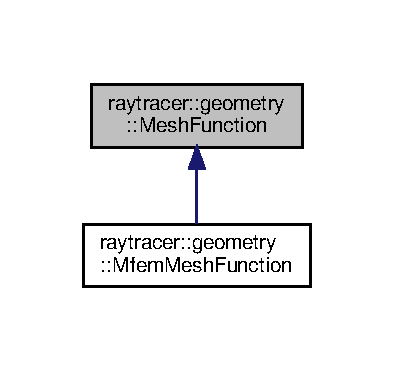
\includegraphics[width=189pt]{classraytracer_1_1geometry_1_1MeshFunction__inherit__graph}
\end{center}
\end{figure}
\subsection*{Public Member Functions}
\begin{DoxyCompactItemize}
\item 
virtual double \hyperlink{classraytracer_1_1geometry_1_1MeshFunction_a8e8a42e0d1793e48146ac7aaf98026c4}{get\+Value} (const \hyperlink{classraytracer_1_1geometry_1_1Element}{Element} \&) const =0
\begin{DoxyCompactList}\small\item\em Override this. \end{DoxyCompactList}\item 
virtual void \hyperlink{classraytracer_1_1geometry_1_1MeshFunction_a9e677af2a48d1b372b19fd6462612744}{set\+Value} (const \hyperlink{classraytracer_1_1geometry_1_1Element}{Element} \&, double value)=0
\begin{DoxyCompactList}\small\item\em Override this. \end{DoxyCompactList}\item 
virtual void \hyperlink{classraytracer_1_1geometry_1_1MeshFunction_a5a5908cb7ce59486d3fe987f73d040b6}{add\+Value} (const \hyperlink{classraytracer_1_1geometry_1_1Element}{Element} \&, double value)=0
\begin{DoxyCompactList}\small\item\em Override this. \end{DoxyCompactList}\end{DoxyCompactItemize}


\subsection{Detailed Description}
Abstract interface. 

To obey this \hyperlink{classraytracer_1_1geometry_1_1MeshFunction}{Mesh\+Function} interface get\+Value, set\+Value and add\+Value methods must be implemented. 

\subsection{Member Function Documentation}
\mbox{\Hypertarget{classraytracer_1_1geometry_1_1MeshFunction_a5a5908cb7ce59486d3fe987f73d040b6}\label{classraytracer_1_1geometry_1_1MeshFunction_a5a5908cb7ce59486d3fe987f73d040b6}} 
\index{raytracer\+::geometry\+::\+Mesh\+Function@{raytracer\+::geometry\+::\+Mesh\+Function}!add\+Value@{add\+Value}}
\index{add\+Value@{add\+Value}!raytracer\+::geometry\+::\+Mesh\+Function@{raytracer\+::geometry\+::\+Mesh\+Function}}
\subsubsection{\texorpdfstring{add\+Value()}{addValue()}}
{\footnotesize\ttfamily virtual void raytracer\+::geometry\+::\+Mesh\+Function\+::add\+Value (\begin{DoxyParamCaption}\item[{const \hyperlink{classraytracer_1_1geometry_1_1Element}{Element} \&}]{,  }\item[{double}]{value }\end{DoxyParamCaption})\hspace{0.3cm}{\ttfamily [pure virtual]}}



Override this. 


\begin{DoxyParams}{Parameters}
{\em value} & to be added to current value at element. \\
\hline
\end{DoxyParams}


Implemented in \hyperlink{classraytracer_1_1geometry_1_1MfemMeshFunction_a886efe65ad4667b09e00381c57bb7be8}{raytracer\+::geometry\+::\+Mfem\+Mesh\+Function}.

\mbox{\Hypertarget{classraytracer_1_1geometry_1_1MeshFunction_a8e8a42e0d1793e48146ac7aaf98026c4}\label{classraytracer_1_1geometry_1_1MeshFunction_a8e8a42e0d1793e48146ac7aaf98026c4}} 
\index{raytracer\+::geometry\+::\+Mesh\+Function@{raytracer\+::geometry\+::\+Mesh\+Function}!get\+Value@{get\+Value}}
\index{get\+Value@{get\+Value}!raytracer\+::geometry\+::\+Mesh\+Function@{raytracer\+::geometry\+::\+Mesh\+Function}}
\subsubsection{\texorpdfstring{get\+Value()}{getValue()}}
{\footnotesize\ttfamily virtual double raytracer\+::geometry\+::\+Mesh\+Function\+::get\+Value (\begin{DoxyParamCaption}\item[{const \hyperlink{classraytracer_1_1geometry_1_1Element}{Element} \&}]{ }\end{DoxyParamCaption}) const\hspace{0.3cm}{\ttfamily [pure virtual]}}



Override this. 

\begin{DoxyReturn}{Returns}
value of \hyperlink{classraytracer_1_1geometry_1_1MeshFunction}{Mesh\+Function} at element 
\end{DoxyReturn}


Implemented in \hyperlink{classraytracer_1_1geometry_1_1MfemMeshFunction_a76b37f146c8471f95c0e2486024857f7}{raytracer\+::geometry\+::\+Mfem\+Mesh\+Function}.

\mbox{\Hypertarget{classraytracer_1_1geometry_1_1MeshFunction_a9e677af2a48d1b372b19fd6462612744}\label{classraytracer_1_1geometry_1_1MeshFunction_a9e677af2a48d1b372b19fd6462612744}} 
\index{raytracer\+::geometry\+::\+Mesh\+Function@{raytracer\+::geometry\+::\+Mesh\+Function}!set\+Value@{set\+Value}}
\index{set\+Value@{set\+Value}!raytracer\+::geometry\+::\+Mesh\+Function@{raytracer\+::geometry\+::\+Mesh\+Function}}
\subsubsection{\texorpdfstring{set\+Value()}{setValue()}}
{\footnotesize\ttfamily virtual void raytracer\+::geometry\+::\+Mesh\+Function\+::set\+Value (\begin{DoxyParamCaption}\item[{const \hyperlink{classraytracer_1_1geometry_1_1Element}{Element} \&}]{,  }\item[{double}]{value }\end{DoxyParamCaption})\hspace{0.3cm}{\ttfamily [pure virtual]}}



Override this. 


\begin{DoxyParams}{Parameters}
{\em value} & value to be set at element \\
\hline
\end{DoxyParams}


Implemented in \hyperlink{classraytracer_1_1geometry_1_1MfemMeshFunction_a3153afe8fbdf71f1f5f7d7a44c507536}{raytracer\+::geometry\+::\+Mfem\+Mesh\+Function}.



The documentation for this class was generated from the following file\+:\begin{DoxyCompactItemize}
\item 
include/raytracer/geometry/Mesh\+Function.\+h\end{DoxyCompactItemize}

\hypertarget{classraytracer_1_1geometry_1_1MfemMeshFunction}{}\section{raytracer\+:\+:geometry\+:\+:Mfem\+Mesh\+Function Class Reference}
\label{classraytracer_1_1geometry_1_1MfemMeshFunction}\index{raytracer\+::geometry\+::\+Mfem\+Mesh\+Function@{raytracer\+::geometry\+::\+Mfem\+Mesh\+Function}}


Wrapper class around mfem\+::\+Grid\+Function.  




{\ttfamily \#include $<$Mesh\+Function.\+h$>$}



Inheritance diagram for raytracer\+:\+:geometry\+:\+:Mfem\+Mesh\+Function\+:\nopagebreak
\begin{figure}[H]
\begin{center}
\leavevmode
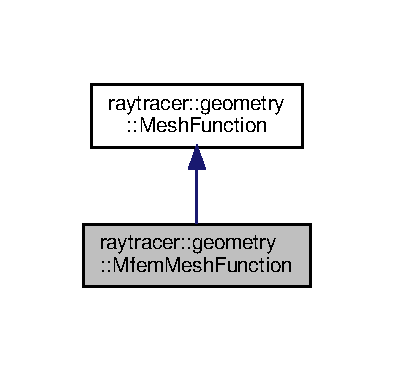
\includegraphics[width=189pt]{classraytracer_1_1geometry_1_1MfemMeshFunction__inherit__graph}
\end{center}
\end{figure}


Collaboration diagram for raytracer\+:\+:geometry\+:\+:Mfem\+Mesh\+Function\+:\nopagebreak
\begin{figure}[H]
\begin{center}
\leavevmode
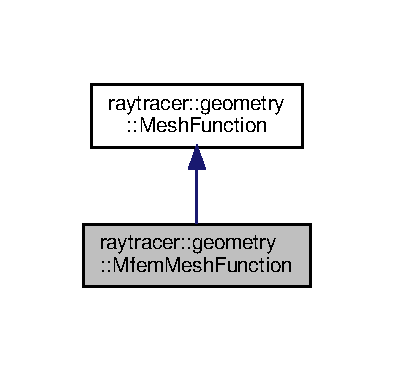
\includegraphics[width=189pt]{classraytracer_1_1geometry_1_1MfemMeshFunction__coll__graph}
\end{center}
\end{figure}
\subsection*{Public Member Functions}
\begin{DoxyCompactItemize}
\item 
\hyperlink{classraytracer_1_1geometry_1_1MfemMeshFunction_a38898aa9932de5f6d8ceecdf27d26761}{Mfem\+Mesh\+Function} (mfem\+::\+Grid\+Function \&grid\+Function, const mfem\+::\+Finite\+Element\+Space \&finite\+Element\+Space)
\begin{DoxyCompactList}\small\item\em Create the \hyperlink{classraytracer_1_1geometry_1_1MeshFunction}{Mesh\+Function} from a mfem\+::\+Grid\+Function and mfem\+::\+Finite\+Element\+Space. \end{DoxyCompactList}\item 
double \hyperlink{classraytracer_1_1geometry_1_1MfemMeshFunction_a76b37f146c8471f95c0e2486024857f7}{get\+Value} (const \hyperlink{classraytracer_1_1geometry_1_1Element}{Element} \&element) const override
\begin{DoxyCompactList}\small\item\em Get a value of mfem\+::\+Grid\+Function based on an element. \end{DoxyCompactList}\item 
void \hyperlink{classraytracer_1_1geometry_1_1MfemMeshFunction_a3153afe8fbdf71f1f5f7d7a44c507536}{set\+Value} (const \hyperlink{classraytracer_1_1geometry_1_1Element}{Element} \&element, double value) override
\begin{DoxyCompactList}\small\item\em Set a value of mfem\+::\+Grid\+Function based on an element. \end{DoxyCompactList}\item 
void \hyperlink{classraytracer_1_1geometry_1_1MfemMeshFunction_a886efe65ad4667b09e00381c57bb7be8}{add\+Value} (const \hyperlink{classraytracer_1_1geometry_1_1Element}{Element} \&element, double value) override
\begin{DoxyCompactList}\small\item\em Add a value to existing value of mfem\+::\+Grid\+Function based on an element. \end{DoxyCompactList}\end{DoxyCompactItemize}


\subsection{Detailed Description}
Wrapper class around mfem\+::\+Grid\+Function. 

Provides a way to query the Grid\+Function given an element. 

\subsection{Constructor \& Destructor Documentation}
\mbox{\Hypertarget{classraytracer_1_1geometry_1_1MfemMeshFunction_a38898aa9932de5f6d8ceecdf27d26761}\label{classraytracer_1_1geometry_1_1MfemMeshFunction_a38898aa9932de5f6d8ceecdf27d26761}} 
\index{raytracer\+::geometry\+::\+Mfem\+Mesh\+Function@{raytracer\+::geometry\+::\+Mfem\+Mesh\+Function}!Mfem\+Mesh\+Function@{Mfem\+Mesh\+Function}}
\index{Mfem\+Mesh\+Function@{Mfem\+Mesh\+Function}!raytracer\+::geometry\+::\+Mfem\+Mesh\+Function@{raytracer\+::geometry\+::\+Mfem\+Mesh\+Function}}
\subsubsection{\texorpdfstring{Mfem\+Mesh\+Function()}{MfemMeshFunction()}}
{\footnotesize\ttfamily raytracer\+::geometry\+::\+Mfem\+Mesh\+Function\+::\+Mfem\+Mesh\+Function (\begin{DoxyParamCaption}\item[{mfem\+::\+Grid\+Function \&}]{grid\+Function,  }\item[{const mfem\+::\+Finite\+Element\+Space \&}]{finite\+Element\+Space }\end{DoxyParamCaption})\hspace{0.3cm}{\ttfamily [explicit]}}



Create the \hyperlink{classraytracer_1_1geometry_1_1MeshFunction}{Mesh\+Function} from a mfem\+::\+Grid\+Function and mfem\+::\+Finite\+Element\+Space. 


\begin{DoxyParams}{Parameters}
{\em grid\+Function} & a mutable reference will be kept. \\
\hline
{\em finite\+Element\+Space} & const reference will be kept -\/ caution\+: L2 space is expected! \\
\hline
\end{DoxyParams}


\subsection{Member Function Documentation}
\mbox{\Hypertarget{classraytracer_1_1geometry_1_1MfemMeshFunction_a886efe65ad4667b09e00381c57bb7be8}\label{classraytracer_1_1geometry_1_1MfemMeshFunction_a886efe65ad4667b09e00381c57bb7be8}} 
\index{raytracer\+::geometry\+::\+Mfem\+Mesh\+Function@{raytracer\+::geometry\+::\+Mfem\+Mesh\+Function}!add\+Value@{add\+Value}}
\index{add\+Value@{add\+Value}!raytracer\+::geometry\+::\+Mfem\+Mesh\+Function@{raytracer\+::geometry\+::\+Mfem\+Mesh\+Function}}
\subsubsection{\texorpdfstring{add\+Value()}{addValue()}}
{\footnotesize\ttfamily void raytracer\+::geometry\+::\+Mfem\+Mesh\+Function\+::add\+Value (\begin{DoxyParamCaption}\item[{const \hyperlink{classraytracer_1_1geometry_1_1Element}{Element} \&}]{element,  }\item[{double}]{value }\end{DoxyParamCaption})\hspace{0.3cm}{\ttfamily [override]}, {\ttfamily [virtual]}}



Add a value to existing value of mfem\+::\+Grid\+Function based on an element. 


\begin{DoxyParams}{Parameters}
{\em element} & \\
\hline
{\em value} & \\
\hline
\end{DoxyParams}


Implements \hyperlink{classraytracer_1_1geometry_1_1MeshFunction_a5a5908cb7ce59486d3fe987f73d040b6}{raytracer\+::geometry\+::\+Mesh\+Function}.

\mbox{\Hypertarget{classraytracer_1_1geometry_1_1MfemMeshFunction_a76b37f146c8471f95c0e2486024857f7}\label{classraytracer_1_1geometry_1_1MfemMeshFunction_a76b37f146c8471f95c0e2486024857f7}} 
\index{raytracer\+::geometry\+::\+Mfem\+Mesh\+Function@{raytracer\+::geometry\+::\+Mfem\+Mesh\+Function}!get\+Value@{get\+Value}}
\index{get\+Value@{get\+Value}!raytracer\+::geometry\+::\+Mfem\+Mesh\+Function@{raytracer\+::geometry\+::\+Mfem\+Mesh\+Function}}
\subsubsection{\texorpdfstring{get\+Value()}{getValue()}}
{\footnotesize\ttfamily double raytracer\+::geometry\+::\+Mfem\+Mesh\+Function\+::get\+Value (\begin{DoxyParamCaption}\item[{const \hyperlink{classraytracer_1_1geometry_1_1Element}{Element} \&}]{element }\end{DoxyParamCaption}) const\hspace{0.3cm}{\ttfamily [override]}, {\ttfamily [virtual]}}



Get a value of mfem\+::\+Grid\+Function based on an element. 


\begin{DoxyParams}{Parameters}
{\em element} & \\
\hline
\end{DoxyParams}
\begin{DoxyReturn}{Returns}
the value of Grid\+Function at the element true dof. 
\end{DoxyReturn}


Implements \hyperlink{classraytracer_1_1geometry_1_1MeshFunction_a8e8a42e0d1793e48146ac7aaf98026c4}{raytracer\+::geometry\+::\+Mesh\+Function}.

\mbox{\Hypertarget{classraytracer_1_1geometry_1_1MfemMeshFunction_a3153afe8fbdf71f1f5f7d7a44c507536}\label{classraytracer_1_1geometry_1_1MfemMeshFunction_a3153afe8fbdf71f1f5f7d7a44c507536}} 
\index{raytracer\+::geometry\+::\+Mfem\+Mesh\+Function@{raytracer\+::geometry\+::\+Mfem\+Mesh\+Function}!set\+Value@{set\+Value}}
\index{set\+Value@{set\+Value}!raytracer\+::geometry\+::\+Mfem\+Mesh\+Function@{raytracer\+::geometry\+::\+Mfem\+Mesh\+Function}}
\subsubsection{\texorpdfstring{set\+Value()}{setValue()}}
{\footnotesize\ttfamily void raytracer\+::geometry\+::\+Mfem\+Mesh\+Function\+::set\+Value (\begin{DoxyParamCaption}\item[{const \hyperlink{classraytracer_1_1geometry_1_1Element}{Element} \&}]{element,  }\item[{double}]{value }\end{DoxyParamCaption})\hspace{0.3cm}{\ttfamily [override]}, {\ttfamily [virtual]}}



Set a value of mfem\+::\+Grid\+Function based on an element. 


\begin{DoxyParams}{Parameters}
{\em element} & \\
\hline
{\em value} & \\
\hline
\end{DoxyParams}


Implements \hyperlink{classraytracer_1_1geometry_1_1MeshFunction_a9e677af2a48d1b372b19fd6462612744}{raytracer\+::geometry\+::\+Mesh\+Function}.



The documentation for this class was generated from the following file\+:\begin{DoxyCompactItemize}
\item 
include/raytracer/geometry/Mesh\+Function.\+h\end{DoxyCompactItemize}

\hypertarget{classraytracer_1_1geometry_1_1Point}{}\section{raytracer\+:\+:geometry\+:\+:Point Class Reference}
\label{classraytracer_1_1geometry_1_1Point}\index{raytracer\+::geometry\+::\+Point@{raytracer\+::geometry\+::\+Point}}


Class representing a point A point is given by two coordinates x and y.  




{\ttfamily \#include $<$Point.\+h$>$}

\subsection*{Public Member Functions}
\begin{DoxyCompactItemize}
\item 
\hyperlink{classraytracer_1_1geometry_1_1Point_ad05a2dc2f77d1a2720a6dd19a6b1c5ed}{Point} (double \hyperlink{classraytracer_1_1geometry_1_1Point_a1408a40033e6273f93e539875dfe09b3}{x}, double \hyperlink{classraytracer_1_1geometry_1_1Point_a7fcd0651b22e64147a33dded20b72fd1}{y})
\begin{DoxyCompactList}\small\item\em Construct the edge fiven x and y. \end{DoxyCompactList}\item 
\hyperlink{classraytracer_1_1geometry_1_1Point_ac8c3dcaf9edb06b36bf3301348eb946a}{Point} ()=default
\begin{DoxyCompactList}\small\item\em Default contructor. \end{DoxyCompactList}\item 
bool \hyperlink{classraytracer_1_1geometry_1_1Point_ae363ee68a65544c87142d64433d790e0}{operator==} (const \hyperlink{classraytracer_1_1geometry_1_1Point}{Point} \&another\+Point) const
\begin{DoxyCompactList}\small\item\em Equality operator. \end{DoxyCompactList}\end{DoxyCompactItemize}
\subsection*{Public Attributes}
\begin{DoxyCompactItemize}
\item 
\mbox{\Hypertarget{classraytracer_1_1geometry_1_1Point_a1408a40033e6273f93e539875dfe09b3}\label{classraytracer_1_1geometry_1_1Point_a1408a40033e6273f93e539875dfe09b3}} 
double \hyperlink{classraytracer_1_1geometry_1_1Point_a1408a40033e6273f93e539875dfe09b3}{x}
\begin{DoxyCompactList}\small\item\em x coordinate \end{DoxyCompactList}\item 
\mbox{\Hypertarget{classraytracer_1_1geometry_1_1Point_a7fcd0651b22e64147a33dded20b72fd1}\label{classraytracer_1_1geometry_1_1Point_a7fcd0651b22e64147a33dded20b72fd1}} 
double \hyperlink{classraytracer_1_1geometry_1_1Point_a7fcd0651b22e64147a33dded20b72fd1}{y}
\begin{DoxyCompactList}\small\item\em y coordinate \end{DoxyCompactList}\end{DoxyCompactItemize}


\subsection{Detailed Description}
Class representing a point A point is given by two coordinates x and y. 

\subsection{Constructor \& Destructor Documentation}
\mbox{\Hypertarget{classraytracer_1_1geometry_1_1Point_ad05a2dc2f77d1a2720a6dd19a6b1c5ed}\label{classraytracer_1_1geometry_1_1Point_ad05a2dc2f77d1a2720a6dd19a6b1c5ed}} 
\index{raytracer\+::geometry\+::\+Point@{raytracer\+::geometry\+::\+Point}!Point@{Point}}
\index{Point@{Point}!raytracer\+::geometry\+::\+Point@{raytracer\+::geometry\+::\+Point}}
\subsubsection{\texorpdfstring{Point()}{Point()}\hspace{0.1cm}{\footnotesize\ttfamily [1/2]}}
{\footnotesize\ttfamily raytracer\+::geometry\+::\+Point\+::\+Point (\begin{DoxyParamCaption}\item[{double}]{x,  }\item[{double}]{y }\end{DoxyParamCaption})}



Construct the edge fiven x and y. 

Note that x goes first, be sure not to mix this up. 
\begin{DoxyParams}{Parameters}
{\em x} & coordinate \\
\hline
{\em y} & coordinate \\
\hline
\end{DoxyParams}
\mbox{\Hypertarget{classraytracer_1_1geometry_1_1Point_ac8c3dcaf9edb06b36bf3301348eb946a}\label{classraytracer_1_1geometry_1_1Point_ac8c3dcaf9edb06b36bf3301348eb946a}} 
\index{raytracer\+::geometry\+::\+Point@{raytracer\+::geometry\+::\+Point}!Point@{Point}}
\index{Point@{Point}!raytracer\+::geometry\+::\+Point@{raytracer\+::geometry\+::\+Point}}
\subsubsection{\texorpdfstring{Point()}{Point()}\hspace{0.1cm}{\footnotesize\ttfamily [2/2]}}
{\footnotesize\ttfamily raytracer\+::geometry\+::\+Point\+::\+Point (\begin{DoxyParamCaption}{ }\end{DoxyParamCaption})\hspace{0.3cm}{\ttfamily [default]}}



Default contructor. 

Default contructed point has both x and y equal to 0 

\subsection{Member Function Documentation}
\mbox{\Hypertarget{classraytracer_1_1geometry_1_1Point_ae363ee68a65544c87142d64433d790e0}\label{classraytracer_1_1geometry_1_1Point_ae363ee68a65544c87142d64433d790e0}} 
\index{raytracer\+::geometry\+::\+Point@{raytracer\+::geometry\+::\+Point}!operator==@{operator==}}
\index{operator==@{operator==}!raytracer\+::geometry\+::\+Point@{raytracer\+::geometry\+::\+Point}}
\subsubsection{\texorpdfstring{operator==()}{operator==()}}
{\footnotesize\ttfamily bool raytracer\+::geometry\+::\+Point\+::operator== (\begin{DoxyParamCaption}\item[{const \hyperlink{classraytracer_1_1geometry_1_1Point}{Point} \&}]{another\+Point }\end{DoxyParamCaption}) const}



Equality operator. 

Two points are equal if their coordinates difference is less than given project wide epsilon (defined in constants) 
\begin{DoxyParams}{Parameters}
{\em another\+Point} & to comapre with \\
\hline
\end{DoxyParams}
\begin{DoxyReturn}{Returns}
true if they almost equal 
\end{DoxyReturn}


The documentation for this class was generated from the following file\+:\begin{DoxyCompactItemize}
\item 
include/raytracer/geometry/Point.\+h\end{DoxyCompactItemize}

\hypertarget{classraytracer_1_1geometry_1_1Ray}{}\section{raytracer\+:\+:geometry\+:\+:Ray Class Reference}
\label{classraytracer_1_1geometry_1_1Ray}\index{raytracer\+::geometry\+::\+Ray@{raytracer\+::geometry\+::\+Ray}}


Class representing a ray propagating through mesh.  




{\ttfamily \#include $<$Ray.\+h$>$}

\subsection*{Public Member Functions}
\begin{DoxyCompactItemize}
\item 
\hyperlink{classraytracer_1_1geometry_1_1Ray_a587ca5392f26083838630091f254cbdb}{Ray} (const \hyperlink{structraytracer_1_1geometry_1_1HalfLine}{Half\+Line} \&initial\+Ray)
\begin{DoxyCompactList}\small\item\em Construct it using a \hyperlink{structraytracer_1_1geometry_1_1HalfLine}{Half\+Line} (that is the initial orientation of the \hyperlink{classraytracer_1_1geometry_1_1Ray}{Ray}) \end{DoxyCompactList}\item 
{\footnotesize template$<$typename Inters\+Func , typename Stop\+Condition $>$ }\\std\+::vector$<$ \hyperlink{structraytracer_1_1geometry_1_1Intersection}{Intersection} $>$ \hyperlink{classraytracer_1_1geometry_1_1Ray_a8440acf0af92e6c0718cb137db5e283e}{find\+Intersections} (const \hyperlink{classraytracer_1_1geometry_1_1Mesh}{Mesh} \&mesh, Inters\+Func find\+Inters, Stop\+Condition stop\+Condition)
\begin{DoxyCompactList}\small\item\em Given a mesh direction\+Function and stop\+Condition find all intersections of the ray with a mesh. \end{DoxyCompactList}\end{DoxyCompactItemize}


\subsection{Detailed Description}
Class representing a ray propagating through mesh. 

Here the convention is such that the ray is made up of segments. In general it is not a line and must not be straight. 

\subsection{Constructor \& Destructor Documentation}
\mbox{\Hypertarget{classraytracer_1_1geometry_1_1Ray_a587ca5392f26083838630091f254cbdb}\label{classraytracer_1_1geometry_1_1Ray_a587ca5392f26083838630091f254cbdb}} 
\index{raytracer\+::geometry\+::\+Ray@{raytracer\+::geometry\+::\+Ray}!Ray@{Ray}}
\index{Ray@{Ray}!raytracer\+::geometry\+::\+Ray@{raytracer\+::geometry\+::\+Ray}}
\subsubsection{\texorpdfstring{Ray()}{Ray()}}
{\footnotesize\ttfamily raytracer\+::geometry\+::\+Ray\+::\+Ray (\begin{DoxyParamCaption}\item[{const \hyperlink{structraytracer_1_1geometry_1_1HalfLine}{Half\+Line} \&}]{initial\+Ray }\end{DoxyParamCaption})\hspace{0.3cm}{\ttfamily [inline]}, {\ttfamily [explicit]}}



Construct it using a \hyperlink{structraytracer_1_1geometry_1_1HalfLine}{Half\+Line} (that is the initial orientation of the \hyperlink{classraytracer_1_1geometry_1_1Ray}{Ray}) 


\begin{DoxyParams}{Parameters}
{\em initial\+Ray} & \\
\hline
\end{DoxyParams}


\subsection{Member Function Documentation}
\mbox{\Hypertarget{classraytracer_1_1geometry_1_1Ray_a8440acf0af92e6c0718cb137db5e283e}\label{classraytracer_1_1geometry_1_1Ray_a8440acf0af92e6c0718cb137db5e283e}} 
\index{raytracer\+::geometry\+::\+Ray@{raytracer\+::geometry\+::\+Ray}!find\+Intersections@{find\+Intersections}}
\index{find\+Intersections@{find\+Intersections}!raytracer\+::geometry\+::\+Ray@{raytracer\+::geometry\+::\+Ray}}
\subsubsection{\texorpdfstring{find\+Intersections()}{findIntersections()}}
{\footnotesize\ttfamily template$<$typename Inters\+Func , typename Stop\+Condition $>$ \\
std\+::vector$<$\hyperlink{structraytracer_1_1geometry_1_1Intersection}{Intersection}$>$ raytracer\+::geometry\+::\+Ray\+::find\+Intersections (\begin{DoxyParamCaption}\item[{const \hyperlink{classraytracer_1_1geometry_1_1Mesh}{Mesh} \&}]{mesh,  }\item[{Inters\+Func}]{find\+Inters,  }\item[{Stop\+Condition}]{stop\+Condition }\end{DoxyParamCaption})\hspace{0.3cm}{\ttfamily [inline]}}



Given a mesh direction\+Function and stop\+Condition find all intersections of the ray with a mesh. 

Parameter find\+Inters must be a function with the following signature\+: (const \hyperlink{structraytracer_1_1geometry_1_1Intersection}{Intersection}\& previous\+Intersection, const \hyperlink{classraytracer_1_1geometry_1_1Element}{Element}\& element) -\/$>$ \hyperlink{classraytracer_1_1geometry_1_1Vector}{Vector}. The returned \hyperlink{classraytracer_1_1geometry_1_1Vector}{Vector} is the next direction in which the ray should propagate.

Parameter stop\+Condition must be a function with the following signature\+: (const \hyperlink{structraytracer_1_1geometry_1_1Intersection}{Intersection}\& previous\+Intersection, const \hyperlink{classraytracer_1_1geometry_1_1Element}{Element}\& element) -\/$>$ bool. It should return true if the the ray propagation is to be stopped. Else it has no effect.


\begin{DoxyTemplParams}{Template Parameters}
{\em Inters\+Func} & Generic type used to represent a function \\
\hline
{\em Stop\+Condition} & Generic type used to represent a function \\
\hline
\end{DoxyTemplParams}

\begin{DoxyParams}{Parameters}
{\em mesh} & to be intersected \\
\hline
{\em find\+Inters} & function with signature (const \hyperlink{structraytracer_1_1geometry_1_1Intersection}{Intersection}\& previous\+Intersection, const \hyperlink{classraytracer_1_1geometry_1_1Element}{Element}\& element) -\/$>$ \hyperlink{classraytracer_1_1geometry_1_1Vector}{Vector} \\
\hline
{\em stop\+Condition} & function with signature (const \hyperlink{structraytracer_1_1geometry_1_1Intersection}{Intersection}\& previous\+Intersection, const \hyperlink{classraytracer_1_1geometry_1_1Element}{Element}\& element) -\/$>$ bool. \\
\hline
\end{DoxyParams}
\begin{DoxyReturn}{Returns}
sequence of found intersections 
\end{DoxyReturn}


The documentation for this class was generated from the following file\+:\begin{DoxyCompactItemize}
\item 
include/raytracer/geometry/Ray.\+h\end{DoxyCompactItemize}

\hypertarget{structraytracer_1_1physics_1_1SnellsLaw}{}\section{raytracer\+:\+:physics\+:\+:Snells\+Law Struct Reference}
\label{structraytracer_1_1physics_1_1SnellsLaw}\index{raytracer\+::physics\+::\+Snells\+Law@{raytracer\+::physics\+::\+Snells\+Law}}


Functor that given an intersection finds next intersection base on the Snells\textquotesingle{}s law.  




{\ttfamily \#include $<$Laser\+Propagation.\+h$>$}

\subsection*{Public Member Functions}
\begin{DoxyCompactItemize}
\item 
\hyperlink{structraytracer_1_1physics_1_1SnellsLaw_a43fd9b6200b38980cee85d3451ef125a}{Snells\+Law} (const \hyperlink{classraytracer_1_1geometry_1_1MeshFunction}{geometry\+::\+Mesh\+Function} \&density, const \hyperlink{classraytracer_1_1geometry_1_1MeshFunction}{geometry\+::\+Mesh\+Function} \&temperature, const \hyperlink{classraytracer_1_1geometry_1_1MeshFunction}{geometry\+::\+Mesh\+Function} \&ionization, const \hyperlink{classraytracer_1_1physics_1_1GradientCalculator}{Gradient\+Calculator} \&gradient\+Calculator, const \hyperlink{classraytracer_1_1physics_1_1CollisionalFrequencyCalculator}{Collisional\+Frequency\+Calculator} \&collisional\+Frequency\+Calculator)
\begin{DoxyCompactList}\small\item\em Construct the \hyperlink{structraytracer_1_1physics_1_1SnellsLaw}{Snells\+Law} using the density and temperature function reference. \end{DoxyCompactList}\item 
std\+::unique\+\_\+ptr$<$ \hyperlink{structraytracer_1_1geometry_1_1Intersection}{geometry\+::\+Intersection} $>$ \hyperlink{structraytracer_1_1physics_1_1SnellsLaw_a7e46909c41385ab586a800dd6f8c0b28}{operator()} (const \hyperlink{structraytracer_1_1geometry_1_1Intersection}{geometry\+::\+Intersection} \&intersection, const \hyperlink{structraytracer_1_1physics_1_1LaserRay}{Laser\+Ray} \&laser\+Ray)
\begin{DoxyCompactList}\small\item\em Tries to find another intersection based on Snells law, density (provides an index of rarefaction) and gradient (provides edge direction). \end{DoxyCompactList}\end{DoxyCompactItemize}


\subsection{Detailed Description}
Functor that given an intersection finds next intersection base on the Snells\textquotesingle{}s law. 

\subsection{Constructor \& Destructor Documentation}
\mbox{\Hypertarget{structraytracer_1_1physics_1_1SnellsLaw_a43fd9b6200b38980cee85d3451ef125a}\label{structraytracer_1_1physics_1_1SnellsLaw_a43fd9b6200b38980cee85d3451ef125a}} 
\index{raytracer\+::physics\+::\+Snells\+Law@{raytracer\+::physics\+::\+Snells\+Law}!Snells\+Law@{Snells\+Law}}
\index{Snells\+Law@{Snells\+Law}!raytracer\+::physics\+::\+Snells\+Law@{raytracer\+::physics\+::\+Snells\+Law}}
\subsubsection{\texorpdfstring{Snells\+Law()}{SnellsLaw()}}
{\footnotesize\ttfamily raytracer\+::physics\+::\+Snells\+Law\+::\+Snells\+Law (\begin{DoxyParamCaption}\item[{const \hyperlink{classraytracer_1_1geometry_1_1MeshFunction}{geometry\+::\+Mesh\+Function} \&}]{density,  }\item[{const \hyperlink{classraytracer_1_1geometry_1_1MeshFunction}{geometry\+::\+Mesh\+Function} \&}]{temperature,  }\item[{const \hyperlink{classraytracer_1_1geometry_1_1MeshFunction}{geometry\+::\+Mesh\+Function} \&}]{ionization,  }\item[{const \hyperlink{classraytracer_1_1physics_1_1GradientCalculator}{Gradient\+Calculator} \&}]{gradient\+Calculator,  }\item[{const \hyperlink{classraytracer_1_1physics_1_1CollisionalFrequencyCalculator}{Collisional\+Frequency\+Calculator} \&}]{collisional\+Frequency\+Calculator }\end{DoxyParamCaption})\hspace{0.3cm}{\ttfamily [explicit]}}



Construct the \hyperlink{structraytracer_1_1physics_1_1SnellsLaw}{Snells\+Law} using the density and temperature function reference. 

Provide gradient\+Calculator to calculate the plane of rarefaction. Provide collisional\+Frequency\+Calculator to evaluate the index of rarefaction. \hyperlink{structraytracer_1_1physics_1_1Density}{Density} and temperature values are expected to change. 
\begin{DoxyParams}{Parameters}
{\em density} & \\
\hline
{\em temperature} & \\
\hline
{\em gradient\+Calculator} & \\
\hline
{\em collisional\+Frequency\+Calculator} & \\
\hline
\end{DoxyParams}


\subsection{Member Function Documentation}
\mbox{\Hypertarget{structraytracer_1_1physics_1_1SnellsLaw_a7e46909c41385ab586a800dd6f8c0b28}\label{structraytracer_1_1physics_1_1SnellsLaw_a7e46909c41385ab586a800dd6f8c0b28}} 
\index{raytracer\+::physics\+::\+Snells\+Law@{raytracer\+::physics\+::\+Snells\+Law}!operator()@{operator()}}
\index{operator()@{operator()}!raytracer\+::physics\+::\+Snells\+Law@{raytracer\+::physics\+::\+Snells\+Law}}
\subsubsection{\texorpdfstring{operator()()}{operator()()}}
{\footnotesize\ttfamily std\+::unique\+\_\+ptr$<$\hyperlink{structraytracer_1_1geometry_1_1Intersection}{geometry\+::\+Intersection}$>$ raytracer\+::physics\+::\+Snells\+Law\+::operator() (\begin{DoxyParamCaption}\item[{const \hyperlink{structraytracer_1_1geometry_1_1Intersection}{geometry\+::\+Intersection} \&}]{intersection,  }\item[{const \hyperlink{structraytracer_1_1physics_1_1LaserRay}{Laser\+Ray} \&}]{laser\+Ray }\end{DoxyParamCaption})}



Tries to find another intersection based on Snells law, density (provides an index of rarefaction) and gradient (provides edge direction). 

Could throw error no intersection found! 
\begin{DoxyParams}{Parameters}
{\em intersection} & \\
\hline
{\em laser\+Ray} & \\
\hline
\end{DoxyParams}
\begin{DoxyReturn}{Returns}
found intersection or throw 
\end{DoxyReturn}


The documentation for this struct was generated from the following file\+:\begin{DoxyCompactItemize}
\item 
include/raytracer/physics/Laser\+Propagation.\+h\end{DoxyCompactItemize}

\hypertarget{classraytracer_1_1physics_1_1SpitzerFrequencyCalculator}{}\section{raytracer\+:\+:physics\+:\+:Spitzer\+Frequency\+Calculator Class Reference}
\label{classraytracer_1_1physics_1_1SpitzerFrequencyCalculator}\index{raytracer\+::physics\+::\+Spitzer\+Frequency\+Calculator@{raytracer\+::physics\+::\+Spitzer\+Frequency\+Calculator}}


Inheritance diagram for raytracer\+:\+:physics\+:\+:Spitzer\+Frequency\+Calculator\+:
\nopagebreak
\begin{figure}[H]
\begin{center}
\leavevmode
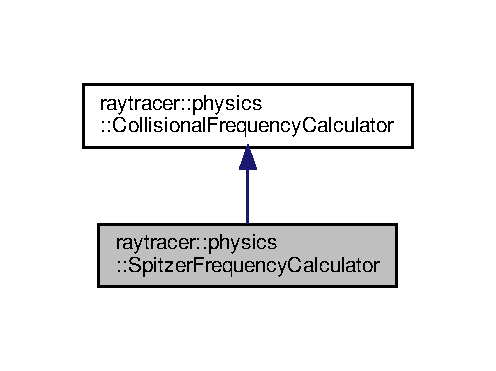
\includegraphics[width=238pt]{classraytracer_1_1physics_1_1SpitzerFrequencyCalculator__inherit__graph}
\end{center}
\end{figure}


Collaboration diagram for raytracer\+:\+:physics\+:\+:Spitzer\+Frequency\+Calculator\+:
\nopagebreak
\begin{figure}[H]
\begin{center}
\leavevmode
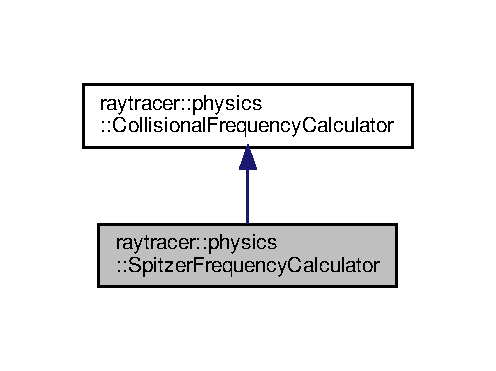
\includegraphics[width=238pt]{classraytracer_1_1physics_1_1SpitzerFrequencyCalculator__coll__graph}
\end{center}
\end{figure}
\subsection*{Public Member Functions}
\begin{DoxyCompactItemize}
\item 
\mbox{\Hypertarget{classraytracer_1_1physics_1_1SpitzerFrequencyCalculator_a709e8207919a6184669e3b3891b65758}\label{classraytracer_1_1physics_1_1SpitzerFrequencyCalculator_a709e8207919a6184669e3b3891b65758}} 
\hyperlink{structraytracer_1_1physics_1_1Frequency}{Frequency} {\bfseries get\+Collisional\+Frequency} (const \hyperlink{structraytracer_1_1physics_1_1Density}{Density} \&density, const \hyperlink{structraytracer_1_1physics_1_1Temperature}{Temperature} \&temperature, const \hyperlink{structraytracer_1_1physics_1_1Length}{Length} \&laser\+Wavelength, double ionization) const override
\end{DoxyCompactItemize}


The documentation for this class was generated from the following file\+:\begin{DoxyCompactItemize}
\item 
include/raytracer/physics/Collisional\+Frequency\+Calculators.\+h\end{DoxyCompactItemize}

\hypertarget{structraytracer_1_1physics_1_1StopAtCritical}{}\section{raytracer\+:\+:physics\+:\+:Stop\+At\+Critical Struct Reference}
\label{structraytracer_1_1physics_1_1StopAtCritical}\index{raytracer\+::physics\+::\+Stop\+At\+Critical@{raytracer\+::physics\+::\+Stop\+At\+Critical}}


Functor for ray propagation termination based on critical density expected to used with lase\+Ray intersection finding procedure.  




{\ttfamily \#include $<$Laser\+Propagation.\+h$>$}

\subsection*{Public Member Functions}
\begin{DoxyCompactItemize}
\item 
\hyperlink{structraytracer_1_1physics_1_1StopAtCritical_adf3b3635cbe76fb2f9a079c27e31f430}{Stop\+At\+Critical} (const \hyperlink{classraytracer_1_1geometry_1_1MeshFunction}{geometry\+::\+Mesh\+Function} \&density)
\begin{DoxyCompactList}\small\item\em Constructor the functor using a density Mesh\+Function. \end{DoxyCompactList}\item 
bool \hyperlink{structraytracer_1_1physics_1_1StopAtCritical_a54e6eb47a50e7448e997444647a900be}{operator()} (const \hyperlink{structraytracer_1_1geometry_1_1Intersection}{geometry\+::\+Intersection} \&intersection, const \hyperlink{structraytracer_1_1physics_1_1LaserRay}{Laser\+Ray} \&laser\+Ray)
\begin{DoxyCompactList}\small\item\em Returns true if the density at the laser\+Ray next element to go to is greater than critical\+Density of the laser ray. \end{DoxyCompactList}\end{DoxyCompactItemize}


\subsection{Detailed Description}
Functor for ray propagation termination based on critical density expected to used with lase\+Ray intersection finding procedure. 

\subsection{Constructor \& Destructor Documentation}
\mbox{\Hypertarget{structraytracer_1_1physics_1_1StopAtCritical_adf3b3635cbe76fb2f9a079c27e31f430}\label{structraytracer_1_1physics_1_1StopAtCritical_adf3b3635cbe76fb2f9a079c27e31f430}} 
\index{raytracer\+::physics\+::\+Stop\+At\+Critical@{raytracer\+::physics\+::\+Stop\+At\+Critical}!Stop\+At\+Critical@{Stop\+At\+Critical}}
\index{Stop\+At\+Critical@{Stop\+At\+Critical}!raytracer\+::physics\+::\+Stop\+At\+Critical@{raytracer\+::physics\+::\+Stop\+At\+Critical}}
\subsubsection{\texorpdfstring{Stop\+At\+Critical()}{StopAtCritical()}}
{\footnotesize\ttfamily raytracer\+::physics\+::\+Stop\+At\+Critical\+::\+Stop\+At\+Critical (\begin{DoxyParamCaption}\item[{const \hyperlink{classraytracer_1_1geometry_1_1MeshFunction}{geometry\+::\+Mesh\+Function} \&}]{density }\end{DoxyParamCaption})\hspace{0.3cm}{\ttfamily [explicit]}}



Constructor the functor using a density Mesh\+Function. 


\begin{DoxyParams}{Parameters}
{\em density} & \\
\hline
\end{DoxyParams}


\subsection{Member Function Documentation}
\mbox{\Hypertarget{structraytracer_1_1physics_1_1StopAtCritical_a54e6eb47a50e7448e997444647a900be}\label{structraytracer_1_1physics_1_1StopAtCritical_a54e6eb47a50e7448e997444647a900be}} 
\index{raytracer\+::physics\+::\+Stop\+At\+Critical@{raytracer\+::physics\+::\+Stop\+At\+Critical}!operator()@{operator()}}
\index{operator()@{operator()}!raytracer\+::physics\+::\+Stop\+At\+Critical@{raytracer\+::physics\+::\+Stop\+At\+Critical}}
\subsubsection{\texorpdfstring{operator()()}{operator()()}}
{\footnotesize\ttfamily bool raytracer\+::physics\+::\+Stop\+At\+Critical\+::operator() (\begin{DoxyParamCaption}\item[{const \hyperlink{structraytracer_1_1geometry_1_1Intersection}{geometry\+::\+Intersection} \&}]{intersection,  }\item[{const \hyperlink{structraytracer_1_1physics_1_1LaserRay}{Laser\+Ray} \&}]{laser\+Ray }\end{DoxyParamCaption})}



Returns true if the density at the laser\+Ray next element to go to is greater than critical\+Density of the laser ray. 


\begin{DoxyParams}{Parameters}
{\em intersection} & current laser\+Ray intersection \\
\hline
{\em laser\+Ray} & \\
\hline
\end{DoxyParams}
\begin{DoxyReturn}{Returns}
true if current density is grater than critical 
\end{DoxyReturn}


The documentation for this struct was generated from the following file\+:\begin{DoxyCompactItemize}
\item 
include/raytracer/physics/Laser\+Propagation.\+h\end{DoxyCompactItemize}

\hypertarget{structraytracer_1_1physics_1_1Temperature}{}\section{raytracer\+:\+:physics\+:\+:Temperature Struct Reference}
\label{structraytracer_1_1physics_1_1Temperature}\index{raytracer\+::physics\+::\+Temperature@{raytracer\+::physics\+::\+Temperature}}


Strong type representing temperature in eV.  




{\ttfamily \#include $<$Magnitudes.\+h$>$}



\subsection{Detailed Description}
Strong type representing temperature in eV. 



The documentation for this struct was generated from the following file\+:\begin{DoxyCompactItemize}
\item 
include/raytracer/physics/Magnitudes.\+h\end{DoxyCompactItemize}

\hypertarget{classraytracer_1_1geometry_1_1Vector}{}\section{raytracer\+:\+:geometry\+:\+:Vector Class Reference}
\label{classraytracer_1_1geometry_1_1Vector}\index{raytracer\+::geometry\+::\+Vector@{raytracer\+::geometry\+::\+Vector}}


Class representing a physical vector.  




{\ttfamily \#include $<$Vector.\+h$>$}

\subsection*{Public Member Functions}
\begin{DoxyCompactItemize}
\item 
\hyperlink{classraytracer_1_1geometry_1_1Vector_acd5cb78949603529e271310395459440}{Vector} (double \hyperlink{classraytracer_1_1geometry_1_1Vector_a954a5ffca3169512b63cf6d2530d957f}{x}, double \hyperlink{classraytracer_1_1geometry_1_1Vector_a6f94f809967bec250380eb2fa91492c2}{y})
\begin{DoxyCompactList}\small\item\em Construct the vector using its coordinates. \end{DoxyCompactList}\item 
\mbox{\Hypertarget{classraytracer_1_1geometry_1_1Vector_a2934dbfb44caa33bf0ac822f97fcd0b6}\label{classraytracer_1_1geometry_1_1Vector_a2934dbfb44caa33bf0ac822f97fcd0b6}} 
\hyperlink{classraytracer_1_1geometry_1_1Vector_a2934dbfb44caa33bf0ac822f97fcd0b6}{Vector} ()=default
\begin{DoxyCompactList}\small\item\em Default constructor initializes a (0, 0) vector. \end{DoxyCompactList}\item 
double \hyperlink{classraytracer_1_1geometry_1_1Vector_ac16dbbd95d3e439c6d4b81bf249d1e83}{get\+Norm} () const
\begin{DoxyCompactList}\small\item\em Return the Euclidean norm of the vector (square root of sum of coordinates squared) \end{DoxyCompactList}\item 
\hyperlink{classraytracer_1_1geometry_1_1Vector}{Vector} \hyperlink{classraytracer_1_1geometry_1_1Vector_a49b341cfda70b916ed0c200feb8bad50}{get\+Normal} () const
\begin{DoxyCompactList}\small\item\em Return the normal to the vector using the convention (y, -\/x) \end{DoxyCompactList}\end{DoxyCompactItemize}
\subsection*{Public Attributes}
\begin{DoxyCompactItemize}
\item 
\mbox{\Hypertarget{classraytracer_1_1geometry_1_1Vector_a954a5ffca3169512b63cf6d2530d957f}\label{classraytracer_1_1geometry_1_1Vector_a954a5ffca3169512b63cf6d2530d957f}} 
double \hyperlink{classraytracer_1_1geometry_1_1Vector_a954a5ffca3169512b63cf6d2530d957f}{x}
\begin{DoxyCompactList}\small\item\em x coordinate \end{DoxyCompactList}\item 
\mbox{\Hypertarget{classraytracer_1_1geometry_1_1Vector_a6f94f809967bec250380eb2fa91492c2}\label{classraytracer_1_1geometry_1_1Vector_a6f94f809967bec250380eb2fa91492c2}} 
double \hyperlink{classraytracer_1_1geometry_1_1Vector_a6f94f809967bec250380eb2fa91492c2}{y}
\begin{DoxyCompactList}\small\item\em y coordinate \end{DoxyCompactList}\end{DoxyCompactItemize}


\subsection{Detailed Description}
Class representing a physical vector. 

\subsection{Constructor \& Destructor Documentation}
\mbox{\Hypertarget{classraytracer_1_1geometry_1_1Vector_acd5cb78949603529e271310395459440}\label{classraytracer_1_1geometry_1_1Vector_acd5cb78949603529e271310395459440}} 
\index{raytracer\+::geometry\+::\+Vector@{raytracer\+::geometry\+::\+Vector}!Vector@{Vector}}
\index{Vector@{Vector}!raytracer\+::geometry\+::\+Vector@{raytracer\+::geometry\+::\+Vector}}
\subsubsection{\texorpdfstring{Vector()}{Vector()}}
{\footnotesize\ttfamily raytracer\+::geometry\+::\+Vector\+::\+Vector (\begin{DoxyParamCaption}\item[{double}]{x,  }\item[{double}]{y }\end{DoxyParamCaption})}



Construct the vector using its coordinates. 


\begin{DoxyParams}{Parameters}
{\em x} & coordinate \\
\hline
{\em y} & coordinate \\
\hline
\end{DoxyParams}


\subsection{Member Function Documentation}
\mbox{\Hypertarget{classraytracer_1_1geometry_1_1Vector_ac16dbbd95d3e439c6d4b81bf249d1e83}\label{classraytracer_1_1geometry_1_1Vector_ac16dbbd95d3e439c6d4b81bf249d1e83}} 
\index{raytracer\+::geometry\+::\+Vector@{raytracer\+::geometry\+::\+Vector}!get\+Norm@{get\+Norm}}
\index{get\+Norm@{get\+Norm}!raytracer\+::geometry\+::\+Vector@{raytracer\+::geometry\+::\+Vector}}
\subsubsection{\texorpdfstring{get\+Norm()}{getNorm()}}
{\footnotesize\ttfamily double raytracer\+::geometry\+::\+Vector\+::get\+Norm (\begin{DoxyParamCaption}{ }\end{DoxyParamCaption}) const}



Return the Euclidean norm of the vector (square root of sum of coordinates squared) 

\begin{DoxyReturn}{Returns}
size of the vector 
\end{DoxyReturn}
\mbox{\Hypertarget{classraytracer_1_1geometry_1_1Vector_a49b341cfda70b916ed0c200feb8bad50}\label{classraytracer_1_1geometry_1_1Vector_a49b341cfda70b916ed0c200feb8bad50}} 
\index{raytracer\+::geometry\+::\+Vector@{raytracer\+::geometry\+::\+Vector}!get\+Normal@{get\+Normal}}
\index{get\+Normal@{get\+Normal}!raytracer\+::geometry\+::\+Vector@{raytracer\+::geometry\+::\+Vector}}
\subsubsection{\texorpdfstring{get\+Normal()}{getNormal()}}
{\footnotesize\ttfamily \hyperlink{classraytracer_1_1geometry_1_1Vector}{Vector} raytracer\+::geometry\+::\+Vector\+::get\+Normal (\begin{DoxyParamCaption}{ }\end{DoxyParamCaption}) const\hspace{0.3cm}{\ttfamily [inline]}}



Return the normal to the vector using the convention (y, -\/x) 

\begin{DoxyReturn}{Returns}

\end{DoxyReturn}


The documentation for this class was generated from the following file\+:\begin{DoxyCompactItemize}
\item 
include/raytracer/geometry/Vector.\+h\end{DoxyCompactItemize}

%--- End generated contents ---

% Index
\backmatter
\newpage
\phantomsection
\clearemptydoublepage
\addcontentsline{toc}{chapter}{Index}
\printindex

\end{document}
